% !TeX spellcheck = en_US
% !TEX program = pdflatex
\documentclass[12pt,b5paper,notitlepage]{article}
\usepackage[b5paper, margin={0.5in,0.65in}]{geometry}
%\usepackage{fullpage}
\usepackage{amsmath,amscd,amssymb,amsthm,mathrsfs,amsfonts,layout,indentfirst,graphicx,caption,mathabx, stmaryrd,appendix,calc,imakeidx,upgreek,amsbsy,thmtools} % mathabx for \wtidecheck
%\usepackage{ulem} %wave underline
\usepackage[dvipsnames]{xcolor}
\usepackage{palatino}  %template

\usepackage{slashed} % Dirac operator
\usepackage{mathrsfs} % Enable using \mathscr
%\usepackage{eufrak}  another template/font
\usepackage{extarrows} % long equal sign, \xlongequal{blablabla}
\usepackage{enumitem} % enumerate label change e.g. [label=(\alph*)]  shows (a) (b) 
\usepackage{pifont}

%%%%%%%%%%%%%%%%%%%%%%%%%%%%%%

%\usepackage{fontspec}
%\setmainfont{Palatino Linotype}
%\usepackage{emoji}


% emoji, use lualatex  remove \usepackage{palatino}

%%%%%%%%%%%%%


\usepackage{CJK}   % Chinese package





\usepackage{csquotes} % \begin{displayquote}   \begin{displaycquote}  for quotation
\usepackage{epigraph}   %\epigraph{}{}  for quotation
%\pmb  mandatory math bold 

\usepackage{fancyhdr} % date in footer

%\usepackage{soul}  %\ul underline break line automatically

\usepackage{ulem}  % \uline  underline break line   also    \uwave

\usepackage{relsize} % use \mathlarger \larger \text{\larger[2]$...$} to enlarge the size of math symbols

\usepackage{verbatim}  % comment environment


\usepackage{halloweenmath} % Interesting halloween math symbols

%%%%%%%%%%%%%%%%%%%%%%%%%%%%%%
\usepackage[most]{tcolorbox}
\tcbuselibrary{theorems}
% box around equations   \tcboxmath
%%%%%%%%%%%%%%%%%%%%%%%%%%%%%%%%%%

\usepackage{titlesec}
\usepackage{etoolbox}
\pretocmd{\section}{\label{sec:\thesection}}{}{}



%%%%%%%%%%%%%%%%%%%%%%%%%%%%%
% circled colon and thick colon \hcolondel and \colondel

\usepackage{pdfrender}

\newcommand*{\hollowcolon}{%
	\textpdfrender{
		TextRenderingMode=Stroke,
		LineWidth=.1bp,
	}{:}%
}

\newcommand{\hcolondel}[1]{%
	\mathopen{\hollowcolon}#1\mathclose{\hollowcolon}%
}
\newcommand{\colondel}[1]{%
	\mathopen{:}#1\mathclose{:}%
}

%%%%%%%%%%%%%%%%%%%%%%%%%%%%%%%%


\usepackage{setspace}  
\setstretch{1.6}



\usepackage{tikz}
\usetikzlibrary{fadings}
\usetikzlibrary{patterns}
\usetikzlibrary{shadows.blur}
\usetikzlibrary{shapes}
\usetikzlibrary{positioning}
\usetikzlibrary{decorations.markings}

\usepackage{tikz-cd}
\usepackage[nottoc]{tocbibind}   % Add  reference to ToC


\makeindex


% The following set up the line spaces between items in \thebibliography
\usepackage{lipsum}  
\let\OLDthebibliography\thebibliography
\renewcommand\thebibliography[1]{
	\OLDthebibliography{#1}
	\setlength{\parskip}{0pt}
	\setlength{\itemsep}{2pt} 
}


%\hyperref{page.10}{...}

\allowdisplaybreaks  %allow aligns to break between pages
\usepackage{latexsym}
\usepackage{chngcntr}
\usepackage[colorlinks,linkcolor=blue,anchorcolor=blue, linktocpage,
%pagebackref
]{hyperref}
\hypersetup{ urlcolor=cyan,
	citecolor=[rgb]{0,0.5,0}}


\setcounter{tocdepth}{2}	 %hide subsections in the content


\counterwithin{figure}{section}

\counterwithin*{footnote}{section}   % Footnote numbering is recounted from the beginning of each subsection

\renewcommand\theenumi{(\arabic{enumi})}
\renewcommand\theenumii{\alph(enumii)}
\renewcommand\theenumiii{\roman{enumii})}

%Greek letters counter
\newcounter{greek}
\renewcommand{\thegreek}{
  \ifcase\value{gr}
     $ \alpha $ 
  \or
     $ \beta $ 
  \or
     $ \gamma $ 
  \or
    $\delta  $ 
  \or
    $\epsilon  $ 
  \or
    $\zeta  $ 
  \or
    $\eta  $ 
  \or
    $\theta  $ 
  \or
    $\iota  $ 
  \or
    $\kappa  $ 
  \or
    $\lambda  $ 
  \or
    $\mu  $ 
  \or
    $\nu  $ 
  \or
    $\xi  $ 
  \or
    $\omicron  $ 
  \or
    $\pi  $ 
  \or
    $\rho  $ 
  \or
    $\sigma  $ 
  \or
    $\tau  $ 
  \or
    $\upsilon  $ 
  \or
    $\phi  $ 
  \or
    $\chi  $ 
  \or
    $\psi  $ 
  \or
    $\omega  $ 
  \else
    % 超出范围时的默认输出
    \text{None}
  \fi
}


\pagestyle{plain}

% \captionsetup[figure]
% {
% 	labelsep=none	
% }
% 控制图表结构












\theoremstyle{definition}
\newtheorem{definition}{Definition}[section]
\newtheorem{example}[definition]{Example}
\newtheorem{exercise}[definition]{Exercise}
\newtheorem{remark}[definition]{Remark}
\newtheorem{observation}[definition]{Observation}
\newtheorem{assumption}[definition]{Assumption}
\newtheorem{convention}[definition]{Convention}
\newtheorem{priniple}[definition]{Principle}
\newtheorem{notation}[definition]{Notation}
\newtheorem*{axiom}{Axiom}
\newtheorem{coa}[definition]{Theorem}
\newtheorem{srem}[definition]{$\star$ Remark}
\newtheorem{seg}[definition]{$\star$ Example}
\newtheorem{sexe}[definition]{$\star$ Exercise}
\newtheorem{sdf}[definition]{$\star$ Definition}
\newtheorem{question}{Question}
\theoremstyle{remark}
\newtheorem*{note}{Note}
\newtheorem*{claim}{Claim}


\newtheorem{problem}{\color{red}Problem}[section]
%\renewcommand*{\theprob}{{\color{red}\arabic{section}.\arabic{prob}}}
\newtheorem{sprob}[problem]{\color{red}$\star$ Problem}
%\renewcommand*{\thesprob}{{\color{red}\arabic{section}.\arabic{sprob}}}
% \newtheorem{ssprob}[prob]{$\star\star$ Problem}

\theoremstyle{plain}
\newtheorem{theorem}[definition]{Theorem}
\newtheorem{Conclusion}[definition]{Conclusion}
\newtheorem{thd}[definition]{Theorem-Definition}
\newtheorem{proposition}[definition]{Proposition}
\newtheorem{corollary}[definition]{Corollary}
\newtheorem{lemma}[definition]{Lemma}
\newtheorem{sthm}[definition]{$\star$ Theorem}
\newtheorem{slm}[definition]{$\star$ Lemma}

\newtheorem{spp}[definition]{$\star$ Proposition}
\newtheorem{scoroll∫ary}[definition]{$\star$ Corollary}
\newtheorem{fact}[definition]{Fact}

\newtheorem{cond}{Condition}
\newtheorem{Mthm}{Main Theorem}
\renewcommand{\thecond}{\Alph{cond}} % "letter-numbered" theorems
\renewcommand{\theMthm}{\Alph{Mthm}} % "letter-numbered" theorems


% \usepackage[most]{tcolorbox}
% \usepackage{keytheorems}

% \newkeytheoremstyle{boxthm}
%   {
%     noteseparator={: },
%     notebraces={}{},
%     notefont=\bfseries,
%     headpunct={},
%     bodyfont=\normalfont,
%     tcolorbox, % or tcolorbox={<keys>}
%   }
% \newkeytheorem{theorem}[style=boxthm]

%\substack   multiple lines under sum
%\underset{b}{a}   b is under a


% Remind: \overline{L_0}



\usepackage{calligra}
\DeclareMathOperator{\shom}{\mathscr{H}\text{\kern -3pt {\calligra\large om}}\,}
\DeclareMathOperator{\sext}{\mathscr{E}\text{\kern -3pt {\calligra\large xt}}\,}
\DeclareMathOperator{\Rel}{\mathscr{R}\text{\kern -3pt {\calligra\large el}~}\,}
\DeclareMathOperator{\sann}{\mathscr{A}\text{\kern -3pt {\calligra\large nn}}\,}
\DeclareMathOperator{\send}{\mathscr{E}\text{\kern -3pt {\calligra\large nd}}\,}
\DeclareMathOperator{\stor}{\mathscr{T}\text{\kern -3pt {\calligra\large or}}\,}
%write mathscr Hom (and so on) 

\usepackage{aurical}
\DeclareMathOperator{\VVir}{\text{\Fontlukas V}\text{\kern -0pt {\Fontlukas\large ir}}\,}

\newcommand{\vol}{\text{\Fontlukas V}}
\newcommand{\dvol}{d~\text{\Fontlukas V}}
% perfect Vol symbol

\usepackage{aurical}
\usepackage[T1]{fontenc}








\newcommand{\fk}{\mathfrak}
\newcommand{\mc}{\mathcal}
\newcommand{\wtd}{\widetilde}
\newcommand{\wht}{\widehat}
\newcommand{\wch}{\widecheck}
\newcommand{\ovl}{\overline}
\newcommand{\udl}{\underline}
\newcommand{\tr}{\mathrm{t}} %transpose
\newcommand{\Tr}{\mathrm{Tr}}
\newcommand{\End}{\mathrm{End}} %endomorphism
\newcommand{\idt}{\mathbf{1}}
\newcommand{\id}{\mathrm{id}}
\newcommand{\Hom}{\mathrm{Hom}}
\newcommand{\Conf}{\mathrm{Conf}}
\newcommand{\Res}{\mathrm{Res}}
\newcommand{\res}{\mathrm{res}}
\newcommand{\KZ}{\mathrm{KZ}}
\newcommand{\ev}{\mathrm{ev}}
\newcommand{\coev}{\mathrm{coev}}
\newcommand{\opp}{\mathrm{opp}}
\newcommand{\Rep}{\mathrm{Rep}}
\newcommand{\diag}{\mathrm{diag}}
\newcommand{\Dom}{\mathrm{Dom}}
\newcommand{\loc}{\mathrm{loc}}
\newcommand{\con}{\mathrm{c}}
\newcommand{\uni}{\mathrm{u}}
\newcommand{\ssp}{\mathrm{ss}}
\newcommand{\di}{\slashed d}
\newcommand{\Diffp}{\mathrm{Diff}^+}
\newcommand{\Diff}{\mathrm{Diff}}
\newcommand{\PSU}{\mathrm{PSU}(1,1)}
\newcommand{\Vir}{\mathrm{Vir}}
\newcommand{\Witt}{\mathscr W}
\newcommand{\Span}{\mathrm{Span}}
\newcommand{\pri}{\mathrm{p}}
\newcommand{\ER}{E^1(V)_{\mathbb R}}
\newcommand{\prth}[1]{( {#1})}
\newcommand{\bk}[1]{\langle {#1}\rangle}
\newcommand{\bigbk}[1]{\big\langle {#1}\big\rangle}
\newcommand{\Bigbk}[1]{\Big\langle {#1}\Big\rangle}
\newcommand{\biggbk}[1]{\bigg\langle {#1}\bigg\rangle}
\newcommand{\Biggbk}[1]{\Bigg\langle {#1}\Bigg\rangle}
\newcommand{\GA}{\mathscr G_{\mathcal A}}
\newcommand{\vs}{\varsigma}
\newcommand{\Vect}{\mathrm{Vec}}
\newcommand{\Vectc}{\mathrm{Vec}^{\mathbb C}}
\newcommand{\scr}{\mathscr}
\newcommand{\sjs}{\subset\joinrel\subset}
\newcommand{\Jtd}{\widetilde{\mathcal J}}
\newcommand{\gk}{\mathfrak g}
\newcommand{\hk}{\mathfrak h}
\newcommand{\xk}{\mathfrak x}
\newcommand{\yk}{\mathfrak y}
\newcommand{\zk}{\mathfrak z}
\newcommand{\pk}{\mathfrak p}
\newcommand{\hr}{\mathfrak h_{\mathbb R}}
\newcommand{\Ad}{\mathrm{Ad}}
\newcommand{\DHR}{\mathrm{DHR}_{I_0}}
\newcommand{\Repi}{\mathrm{Rep}_{\wtd I_0}}
\newcommand{\im}{\mathbf{i}}
\newcommand{\Co}{\complement}
%\newcommand{\Cu}{\mathcal C^{\mathrm u}}
\newcommand{\RepV}{\mathrm{Rep}^\uni(V)}
\newcommand{\RepA}{\mathrm{Rep}(\mathcal A)}
\newcommand{\RepN}{\mathrm{Rep}(\mathcal N)}
\newcommand{\RepfA}{\mathrm{Rep}^{\mathrm f}(\mathcal A)}
\newcommand{\RepAU}{\mathrm{Rep}^\uni(A_U)}
\newcommand{\RepU}{\mathrm{Rep}^\uni(U)}
\newcommand{\RepL}{\mathrm{Rep}^{\mathrm{L}}}
\newcommand{\HomL}{\mathrm{Hom}^{\mathrm{L}}}
\newcommand{\EndL}{\mathrm{End}^{\mathrm{L}}}
\newcommand{\Bim}{\mathrm{Bim}}
\newcommand{\BimA}{\mathrm{Bim}^\uni(A)}
%\newcommand{\shom}{\scr Hom}
\newcommand{\divi}{\mathrm{div}}
\newcommand{\sgm}{\varsigma}
\newcommand{\SX}{{S_{\fk X}}}
\newcommand{\DX}{D_{\fk X}}
\newcommand{\mbb}{\mathbb}
\newcommand{\mbf}{\mathbf}
\newcommand{\bsb}{\boldsymbol}
\newcommand{\blt}{\bullet}
\newcommand{\Vbb}{\mathbb V}
\newcommand{\Ubb}{\mathbb U}
\newcommand{\Xbb}{\mathbb X}
\newcommand{\Kbb}{\mathbb K}
\newcommand{\Abb}{\mathbb A}
\newcommand{\Wbb}{\mathbb W}
\newcommand{\Mbb}{\mathbb M}
\newcommand{\Gbb}{\mathbb G}
\newcommand{\Cbb}{\mathbb C}
\newcommand{\Nbb}{\mathbb N}
\newcommand{\Zbb}{\mathbb Z}
\newcommand{\Qbb}{\mathbb Q}
\newcommand{\Pbb}{\mathbb P}
\newcommand{\Rbb}{\mathbb R}
\newcommand{\Ebb}{\mathbb E}
\newcommand{\Dbb}{\mathbb D}
\newcommand{\Hbb}{\mathbb H}
\newcommand{\cbf}{\mathbf c}
\newcommand{\Rbf}{\mathbf R}
\newcommand{\wt}{\mathrm{wt}}
\newcommand{\Lie}{\mathrm{Lie}}
\newcommand{\btl}{\blacktriangleleft}
\newcommand{\btr}{\blacktriangleright}
\newcommand{\svir}{\mathcal V\!\mathit{ir}}
\newcommand{\Ker}{\mathrm{Ker}}
\newcommand{\Cok}{\mathrm{Coker}}
\newcommand{\Sbf}{\mathbf{S}}
\newcommand{\low}{\mathrm{low}}
\newcommand{\Sp}{\mathrm{Sp}}
\newcommand{\Rng}{\mathrm{Rng}}
\newcommand{\vN}{\mathrm{vN}}
\newcommand{\Ebf}{\mathbf E}
\newcommand{\Nbf}{\mathbf N}
\newcommand{\Stb}{\mathrm {Stb}}
\newcommand{\SXb}{{S_{\fk X_b}}}
\newcommand{\pr}{\mathrm {pr}}
\newcommand{\SXtd}{S_{\wtd{\fk X}}}
\newcommand{\univ}{\mathrm {univ}}
\newcommand{\vbf}{\mathbf v}
\newcommand{\ubf}{\mathbf u}
\newcommand{\wbf}{\mathbf w}
\newcommand{\CB}{\mathrm{CB}}
\newcommand{\Perm}{\mathrm{Perm}}
\newcommand{\Orb}{\mathrm{Orb}}
\newcommand{\Lss}{{L_{0,\mathrm{s}}}}
\newcommand{\Lni}{{L_{0,\mathrm{n}}}}
\newcommand{\UPSU}{\widetilde{\mathrm{PSU}}(1,1)}
\newcommand{\Sbb}{{\mathbb S}}
\newcommand{\Gc}{\mathscr G_c}
\newcommand{\Obj}{\mathrm{Obj}}
\newcommand{\bpr}{{}^\backprime}
\newcommand{\fin}{\mathrm{fin}}
\newcommand{\Ann}{\mathrm{Ann}}
\newcommand{\Real}{\mathrm{Re}}
\newcommand{\Imag}{\mathrm{Im}}
%\newcommand{\cl}{\mathrm{cl}}
\newcommand{\Ind}{\mathrm{Ind}}
\newcommand{\Supp}{\mathrm{Supp}}
\newcommand{\Specan}{\mathrm{Specan}}
\newcommand{\red}{\mathrm{red}}
\newcommand{\uph}{\upharpoonright}
\newcommand{\Mor}{\mathrm{Mor}}
\newcommand{\pre}{\mathrm{pre}}
\newcommand{\rank}{\mathrm{rank}}
\newcommand{\Jac}{\mathrm{Jac}}
\newcommand{\emb}{\mathrm{emb}}
\newcommand{\Sg}{\mathrm{Sg}}
\newcommand{\Nzd}{\mathrm{Nzd}}
\newcommand{\Owht}{\widehat{\scr O}}
\newcommand{\Ext}{\mathrm{Ext}}
\newcommand{\Tor}{\mathrm{Tor}}
\newcommand{\Com}{\mathrm{Com}}
\newcommand{\Mod}{\mathrm{Mod}}
\newcommand{\nk}{\mathfrak n}
\newcommand{\mk}{\mathfrak m}
\newcommand{\Ass}{\mathrm{Ass}}
\newcommand{\depth}{\mathrm{depth}}
\newcommand{\Coh}{\mathrm{Coh}}
\newcommand{\Gode}{\mathrm{Gode}}
\newcommand{\Fbb}{\mathbb F}
\newcommand{\sgn}{\mathrm{sgn}}
\newcommand{\Aut}{\mathrm{Aut}}
\newcommand{\Modf}{\mathrm{Mod}^{\mathrm f}}
\newcommand{\codim}{\mathrm{codim}}
\newcommand{\card}{\mathrm{card}}
\newcommand{\dps}{\displaystyle}
\newcommand{\Int}{\mathrm{Int}}
\newcommand{\Nbh}{\mathrm{Nbh}}
\newcommand{\Pnbh}{\mathrm{PNbh}}
\newcommand{\Cl}{\mathrm{Cl}}
\newcommand{\diam}{\mathrm{diam}}
\newcommand{\eps}{\varepsilon}
\newcommand{\Vol}{\mathrm{Vol}}
\newcommand{\LSC}{\mathrm{LSC}}
\newcommand{\USC}{\mathrm{USC}}
\newcommand{\Ess}{\mathrm{Rng}^{\mathrm{ess}}}
\newcommand{\Jbf}{\mathbf{J}}
\newcommand{\SL}{\mathrm{SL}}
\newcommand{\GL}{\mathrm{GL}}
\newcommand{\Lin}{\mathrm{Lin}}
\newcommand{\ALin}{\mathrm{ALin}}
\newcommand{\bwn}{\bigwedge\nolimits}
\newcommand{\nbf}{\mathbf n}
\newcommand{\dive}{\mathrm{div}}
\newcommand{\Ln}{\mathrm{Ln}}

\renewcommand{\epsilon}{\varepsilon}






\usepackage{tipa} % wierd symboles e.g. \textturnh
\newcommand{\tipar}{\text{\textrtailr}}
\newcommand{\tipaz}{\text{\textctyogh}}
\newcommand{\tipaomega}{\text{\textcloseomega}}
\newcommand{\tipae}{\text{\textrhookschwa}}
\newcommand{\tipaee}{\text{\textreve}}
\newcommand{\tipak}{\text{\texthtk}}
\newcommand{\mol}{\upmu}
\newcommand{\dmol}{d\upmu}




\usepackage{tipx}
\newcommand{\tipxgamma}{\text{\textfrtailgamma}}
\newcommand{\tipxcc}{\text{\textctstretchc}}
\newcommand{\tipxphi}{\text{\textqplig}}



% make some new environment such that we can put line_in math mode in the center.

\newenvironment{Then}
{Then%
\hspace{\stretch{1}}}
{\hspace{\stretch{1}}%
\phantom{Then}}









\numberwithin{equation}{section}
% count the eqation by section countation



\title{Complex Analysis}
\author{
  {{\bf Instructor:} Jianping Jiang}\\
  {{\bf Notes Taker:} Zejin Lin}\\
	{\small \sc Tsinghua University.}\\
	{\small linzj23@mails.tsinghua.edu.cn}\\
  {\small \href{lzjmaths.github.io}{lzjmaths.github.io}}
}

\DeclareMathOperator{\sign}{sign}
\DeclareMathOperator{\dom}{dom}
\DeclareMathOperator{\ran}{ran}
\DeclareMathOperator{\ord}{ord}
\DeclareMathOperator{\img}{Im}
\newcommand{\dd}{\mathrm{d}}
\newcommand{\ie}{ \textit{ i.e. }}
\newcommand{\st}{ \textit{ s.t. }}
\newcommand{\name}[1]{\textbf{#1}\index{#1}}
\newcommand{\subname}[2]{\textbf{#1}\index{#2!#1}}
\renewcommand{\|}{\Vert}
\renewcommand{\Re}{\mathrm{Re}}
\renewcommand{\Im}{\mathrm{Im}}
% \uppercase\expandafter\romannumeral Big roman number
% \usepackage{wrapfig}

\setcounter{section}{1}

\setcounter{tocdepth}{3} 

\begin{document}
\sloppy
\pagenumbering{arabic}
\maketitle
\begin{center}
  If you have any problem or want to cooperate, please contact me.
\end{center}
\tableofcontents
\newpage

%put your code here
\section{Smooth Manifold}
\begin{definition}[Topological manifold]
    A space  $ M  $ is called a topological manifold if 
    \begin{enumerate}
        \item locally Euclidean
        \item Hausdorff
        \item second countable
    \end{enumerate}
\end{definition}
\begin{definition}[Smooth Manifold]
     A smooth structure is given by an equivalence class of smooth atlas  $ \{(U_\alpha,\varphi_\alpha)\} $ \st  $ \varphi_{\alpha\beta}:\varphi_\alpha(U_\alpha\cap U_\beta)\rightarrow \varphi_\beta(U_\alpha\cap U_\beta) $  is smooth  $ \forall \alpha,\beta $.  $ M=\cup U_\alpha $.\\
     A \name{smooth manifold} is a topological manifold with a smooth structure.\\
     Define when a continuous map  $ f:M_1\rightarrow M_2 $ is smooth if  $ \forall (U_1,\varphi_1)\in\mathcal{A}_1,(U_2,\varphi_2)\in\mathcal{A}_2 $, we have  $ \varphi_2\circ f\circ \varphi_1^{-1}:\varphi_1(U_1\cap U_2)\rightarrow \varphi_2(U_1\cap U_2) $ is smooth. 
\end{definition}
\begin{definition}
    Given  $ (M_1,\mathcal{A}_1),(M_2,\mathcal{A}_2) $. A homeomorphism  $ f:M_1\rightarrow M_2 $ is called a diffeomorphism if   $ f $, $ f^{-1} $  is smooth. \\
    In this case we say  $ (M_1,\mathcal{A}_1),(M_2,\mathcal{A}_2) $ are diffeomorphism. 
\end{definition}
\begin{theorem}[Kervaire]
     $ \exists  $ 1 10-dimensional topological manifold without smooth manifold.
\end{theorem}
\begin{theorem}[Milnor]
     $ \exists  $ a smooth manifold  $ M  $ \st  $ M\cong S^7 $ but not in diffeomorphism meaning.  
\end{theorem}
\begin{theorem}[Kervaire-Milnor]
     $ \exists  $ 28 smooth structures (up to orientation preserving diffeomorphism) on  $ S^7 $ 
\end{theorem}
\begin{theorem}[Morse-Birg]
    On  $ S^7  $. If  $ n \leq 3  $, then any  $ n  $-dimensional topological manifold  $ M  $ has a unique smooth structure up to diffeomorphism.
\end{theorem}
\begin{theorem}[Stallings]
    If  $ n\not=4  $, then  $ \exists  $ a unique smooth structure on  $ \mathbb{R}^n  $ up to diffeomorphism.
\end{theorem}
\begin{theorem}[Donaldson-Freedom-Gompf-Faubes]
     $ \exists  $ uncountable smooth structures on  $ \mathbb{R}^4 $ up to diffeomorphism. 
\end{theorem}
\begin{definition}[topological manifold with boundary]
    A space  $ M  $ is called a topological manifold with boundary if 
    \begin{enumerate}
        \item  $ M  $ is Hausdorff
        \item  $ M  $ is second countable 
        \item  $ \forall  p\in M $,  $ \exists   $ a neighbourhood  $ U  $ of  $ p  $ and a homeomorphism  $ \varphi:U\rightarrow V    $  where  $ V  $ is open in  $ \mathbb{H}^n $ 
    \end{enumerate}
    We say a manifold  $ M  $ is closed if  $ M  $ is compact and  $ \partial M  $ is empty.
\end{definition}
Our motivation for studying manifold is to study the space of solution for equations.
\begin{question}
    Given  $ f:\mathbb{R}^n\rightarrow \mathbb{R} $ smooth,  $ q\in \mathbb{R}^n $, when is  $ f^{-1}(q)  $ is a smooth manifold?
\end{question}

For  $ f:U\rightarrow \mathbb{R}^n $ smooth,  $ U  $ open in  $ \mathbb{R}^m $,  the differential of  $ f  $ at  $ p\in U  $ denoted as  $ \mathrm{d}f(p) $.  
\begin{definition}
    We say  $ p\in U  $ is a \textbf{regular point}\index{regular point} of  $ f  $ if  $ \mathrm{d}f(p)  $ is surjective. Otherwise we say  $ p\in U  $ is a \textbf{critical point}\index{critical point}.\\
    A point  $ q\in \mathbb{R}^n  $ is called a \textbf{regular value}\index{regular value} of  $ f  $ if  $ \forall  p\in f^{-1}(q)  $ ,  $ p  $ is a regular point of  $ f $.\\
    A point  $ q\in \mathbb{R}^n  $ is called a \textbf{critical value}\index{critical value} of  $ f  $ if  $ \forall  p\in f^{-1}(q)  $ ,  $ p  $ is a critical point of  $ f $.
\end{definition}
\begin{theorem}[Implicit function theorem]
    If  $ p\in U  $ is a regular point of  $ f:U\rightarrow \mathbb{R}^n  $. Then there exists 
    \begin{itemize}
        \item An open neighbourhood  $ V  $ of  $ p  $ in  $ U  $
        \item An open subset  $ V'  $ of  $ \mathbb{R}^m $
        \item  A diffeomorphism  $ \varphi:V\rightarrow V'  $ such that  $ P\circ \varphi=f $ where  $ P  $ is the projection from  $ \mathbb{R}^m $ to  $ \mathbb{R}^n $. 
    \end{itemize}
    In other words, near a regular point, we can do local coordinate change to turn  $ f  $ into the projection.
\end{theorem}
\begin{remark}
    In particular, we have a homeomorphism
    \[ f^{-1}(f(p))\cap V \xrightarrow[\text{restriction of  $ \varphi $ }]{\cong }\{(x_1,\dots,x_m)\in V'|(x_1,\cdots.x_n)=f(p)\}\]
    \ie if we set  $ M=f^{-1}(f(p)) $, then  $ (M\cap V,\varphi_p) $ is a chart that contains  $ p  $.  
\end{remark}
\begin{corollary}
    If  $ q  $ is a regular value of  $ f:U\rightarrow \mathbb{R}^n $ then  $ f^{-1}(q) $ is a smooth manifold.
\end{corollary}
\begin{remark}
    It suffices to show that the corresponding charts are compatible.
\end{remark}
\begin{theorem}[Sard]
    If  $ f:U\rightarrow \mathbb{R}^n $ is a smooth map, then the set of critical values of  $ f $ has measure $  0 $.
\end{theorem}
\begin{remark}
    For a "generic"  $ q  $,  $ f^{-1}(q)  $ is a manifold of dimension  $ m-n $. 
\end{remark}
\begin{corollary}
    If  $ f:U\rightarrow\mathbb{R}^n $ is smooth and  $ m<n  $ then  $ f(U ) $ has measure $  0  $. 
\end{corollary}

\subsection{Power Series}
\subsubsection{Power series}
\begin{theorem}[Abel's theorem]
If  $ \sum a_n  $ converges, then  $ f(z)=\sum a_nz^n\rightarrow f(1)  $ as  $ z\rightarrow 1  $ in such a way that  $ \frac{|1-z| }{1-|z| } $ remains bounded.
\end{theorem}
\subsection{Exponential, Trigonometric and logorithmic functions}
\subsubsection{Exponential and Trigonometric function}
The \name{exponential function } is defined as the solution if the differential equation
\[\left\{
    \begin{aligned}
        f'(z)=f(z)\\
        f(0)=1
    \end{aligned}
\right.\]
We denote  $ e^z=\exp z=\sum\limits_{n=0}^\infty \frac{z^n}{n!} $.

The \name{trigonometric function} are defined by 
\[\cos z=\frac{e^{iz}+e^{-iz}}{2}\qquad \sin z=\frac{e^{iz}-e^{-iz}}{2i}\]
\subsubsection{Logorithmic Functions}
The \name{logorithmic function}  $ \ln  $ is defined by  $ z=\ln w  $ is a root of the equation  $ e^z=w $.\\
For  $ w\not=0 $, we write  $ z=x+iy $, then 
\[e^{x+iy}=w\Leftrightarrow 
\left\{
    \begin{aligned}
        e^x=|w|\\
        e^{iy}=\frac{w }{|w|}
    \end{aligned}
\right.\]   
The first equation has a unique solution  $ x=\ln|w|  $.

The second equation  $ e^{iy}=\dfrac{w }{|w|}  $ has a unique solution  $ y_0\in [0,2\pi) $.

If we write  $ w=re^{i\theta} $, then  $ x=\ln w,y=\theta =\arg w $.

Thus, for  $ w\not=0  $, we have 
\[\ln w=\ln|w|+i\arg w\]
The function  $ \ln  $ is actually not single-valued. But we can define a single-valued function  $ Ln $ 

We define 
\[a^b=\exp(b\ln a)\]   
We will prove  $ Ln  $ is analytic in  $ \mathbb{C}-(-\infty,0] $ but not continuous in  $ (-\infty,0] $.

$ Ln  $ is the principal branch of the logithm.   
\section{Conformal Mappings}
\subsection{Basic topology}
\subsubsection{Connectedness}
\begin{theorem}
    A nonempty open set in  $ \mathbb{C} $ is connected iff any two of its points can be joined by a polygon  which lies in the set,\ie Connectedness is equivalent to Path Connectedness
\end{theorem}
An nonempty connected subset is called a \name{region}
\subsubsection{Compactness}
\begin{definition}
    A set  $ X  $ is \name{totally bounded } if  $ \forall \epsilon>0  $,  $ X  $ can be covered by finitely many balls of radius  $ \epsilon  $ 
    
\end{definition}
\begin{theorem}
    A set is compact iff it is complete and totally bounded.
\end{theorem}
\begin{theorem}
    A subset  $ X\subset $ is compact iff every infinite sequence of  $ X  $ has a limit point in  $ X  $.
\end{theorem}
\subsubsection{Continuous Functions}
\begin{theorem}
    Continous function maps connected space to connected space.
\end{theorem}
\begin{theorem}
    Continous function maps compact space to compact space.
\end{theorem}
\subsection{Conformality, geometric consequences of the existence of a derivative}
\subsubsection{Arcs and closed curves}
The equation of an \name{arc} r in  $ \mathbb{C} $ can  be represented by one of the terms
\begin{itemize}
    \item  $ x=x(t),y=y(t) $, $ \alpha \leq t  \leq \beta$,  $ x,y $ are continuous at  $ t $
    \item  $ z(t)=x(t)+iy(t) $, $ \alpha \leq t \leq \beta $.
    \item The  continuous mapping  $ \gamma:[\alpha,\beta]\rightarrow \mathbb{C} $. 
\end{itemize}
For a non-decreasing function  $ \varphi:[\alpha,\beta]\rightarrow[\alpha,\beta] $,  $ z=z(\varphi(t)),\alpha' \leq \tau \leq \beta' $ is \name{change of parameter}  of  $ z(t) $.

The change is \name{reversible } iff  $ \varphi  $ is strictly increasing. 

If  $ \gamma  $ is differentiable, then call  $ \gamma  $ a \name{curve}.

$ \gamma  $ is \subname{simple }{curve}, or a   \textbf{Jordan curve}\index{curve!Jordan curve}, if  $ \gamma $ is injective.

$ \gamma  $ is   \textbf{closed curve}\index{curve!closed curve} if  $ \gamma(0)=\gamma(1) $.  
\subsubsection{Analytic Functions in Regions}
A function  $ f  $ is analytic on an arbitrary set  $ A  $ if it is  the restriction to  $ A  $ of a function which is analytic in some open set containing  $ A  $. 
\begin{theorem}
    An analytic function in a region(\ie open and connected) $ \Omega $ whose derivative is 0 must reduce to a constant. The same hold if the real part, the imaginary part, the modulus, or the argument is constant.
\end{theorem}
\subsection{Conformal Mappings}
Suppose  $ f:\Omega\rightarrow \mathbb{C}$ is analytic in  $ \Omega $.  $ r_1=z_1(t),r_2=z_2(t) $, $ \alpha \leq t \leq \beta $.

 $ z_0=z_1(t_0)=z_2(t_0') ,z_1'(t_0)\not=0,z_2'(\hat{t_0})\not=0,\alpha<t_0,\hat{t_0}<\beta$.
 
  $ f'(z_0)\not=0, w_1(t)=f(z_1(t_0)),w_2=f(z_2(\hat(t_0))) $
  
   $ \Gamma_1=\{w_1(t)|\alpha \leq t \leq \beta\} $,  $ \Gamma_2=\{w_2(t)|\alpha \leq t \leq \beta\}$        
   
Then 
\begin{align*}
    w_1'(t)&=f'(z_1(t))z_1'(t)\\
    w_2'(t)&=f'(z_2(\hat{t}))z_2'(\hat{t})
\end{align*}
 $ \Rightarrow  $
 \begin{align*}
    w'_1(t_0)\not=0&,w_2'(t_0)\not=0\\
    \arg w_1'(t_0)&=\arg f'(z_1(t_0))z_1'(t_0)\\
    \arg w_2'(t_0)&=\arg f'(z_2(\hat{t_0}))z_2'(\hat{t_0})
 \end{align*} 
So the "angle"  $ \arg w_1'(t_0)-\arg w_2'(\hat{t_0}=\arg z_1(t_0)-\arg z_2(\hat{t_0}) $ remains the same. \\
Now we give the definition.
\begin{definition}
     $ w=f(z) $ is said to be \name{conformal} in  $ \Omega $ if  $ f  $ is analytic in  $ \Omega  $ and  $ f'(z)\not=0 $ for  $ \forall z\in \Omega$.    
\end{definition}
Easy to prove that linear change of scale at  $ z_0 $  is independent of the direction.\\
\ie  $ |f'(z_0)|=\lim\limits_{z\to z_0}\frac{\delta \sigma}{\delta s} $ 
\subsection{Length and Area}
The \name{length} of a differentiable arc  $ \gamma $ with the equation  $ z(t)=x(t)+iy(t) $, $ a \leq t \leq b $
\[L(\gamma)=\int_{a }^{b }\sqrt{(x'(t))^2+(y'(t))^2}\mathrm{d}t=\int_{a }^{b }|z'(t)|\mathrm{d}t\]   
For  $ \Gamma=f(\gamma) $ where  $ f  $ conformal mapping.\\
Then 
\[L(\Gamma)=\int_{a}^{b}|f'(z(t))|\cdot|z'(t)|\mathrm{d}t\]
The \name{area} of  $ E\subset \mathbb{R} $ is  $ A(E)=\int \int_{E}\mathrm{d}x\mathrm{d}y $\\
Then by the differentiable functional transformation, the area $ \hat{E}=f(E) $ is 
\[A(\hat{E})=\int \int_E|u_xv_y-u_yv_x|\mathrm{d}x\mathrm{d}y\]  
If  $ f  $ is the conformal mapping of an open set containing  $ E  $, then by Caucht-Riemann equation
\[A(\hat{E})=\int\int_E|f'(z)|^2\mathrm{d}x\mathrm{d}y\]
\section{M{\"o}bius Transformation}
Recall that a \name{M{\"o}bius transformation} is a function of the form
\[w=s(z)=\frac{az+b}{cz+d},\quad ad-bc\not=0\]
Then it has an inverse  $ z=S^{-1}(w)=\dfrac{dw-b}{-cw+a} $.\\
We may define  $ S(\infty)=\lim\limits_{z\to \infty}S(z)=\frac{a }{c} $, $ S(\frac{-d }{c})=\infty $ \\
With these definition,  $ S:\hat{\mathbb{C}}\rightarrow\hat{\mathbb{C}} $ is a topological mapping. Here one may use the chordal metric to define the topology.\\
\[S'(z)=\frac{ad-bc}{(cz+d)^2}\]
Then  $ S  $ is conformal in  $ \hat{\mathbb{C}}-\{-\frac{d }{c},\infty\} $.\\
$ w=z+\alpha  $ is called a \name{parallel translation}.

$ w=kz  $ with  $ |k|=1 $ is a \name{rotation}.

$ w=kz $ with  $ k>0  $ is a \name{homothetic transformation}.

$ x=\frac{1 }{z }  $ is called an \name{inversion}.
\begin{proposition}
    Every M{\"o}bius transformation is a composition of the above four operations.
\end{proposition}    
\subsection{Cross ratio}
For three distinct points  $ z_2,z_3,z_4\in\hat{\mathbb{C}} $,we can find a M{\"o}bius transformation  $ S $ such that  $ S(z_2)=0,S(z_3)=1,S(z_4)=\infty $.
\begin{lemma}
    The M{\"o}bius transformation satisfying the above conditions is unique.
\end{lemma}
The \name{cross ratio} $ (z_1,z_2,z_3,z_4) $ is the image  $ z_1 $ under the M{\"o}bius transformation which maps  $ z_2  $ to 1, $ z_3  $ to 0 and $ z_4  $ to  $ \infty $.
\begin{theorem}
    If  $ z_1,z_2,z_3,z_4\in \hat{\mathbb{C}} $  are distinct, and  $ T  $ is any M{\"o}bius transformation, then $ (Tz_1,Tz_2,Tz_3,Tz_4)=(z_1,z_2,z_3,z_4) $. 
\end{theorem} 
\begin{lemma}
    Let  $ T  $ be a M{\"o}bius transformation,  $ T(\mathbb{R}) $ is either a circle or a straight line.
\end{lemma}  
\begin{theorem}
    The cross ratio  $ (z_1,z_2,z_3,z_4) $ is real iff the four points lie on a circle or a straight line.
\end{theorem}
\begin{remark}
    One may prove the theorem by elementary geometry
\end{remark}

\begin{theorem}
    A M{\"o}bius transformation maps circles into circles.
\end{theorem}
\subsubsection{Symmetry}
Suppose  $ T  $ is a M{\"o}bius transformation which maps  $ \hat{\mathbb{R}}  $ onto a circle  $ C $. \\
We say that  $ w=Tz  $ and  $ w^*=T\bar{z} $ are \name{symmetric} w.r.t.  $ C $.
\begin{remark}
    This definition is independent of  $ T $. Suppose  $ S  $ is another M{\"o}bius transformation which maps  $ \hat{\mathbb{R}} $ onto  $ C $, then  $ S^{-1}T $ maps  $ \hat{\mathbb{R}} $ to  $ \hat{\mathbb{R}} $, and this  $ S^{-1}w=S^{-1}Tz $ and  $ S^{-1}w^*=S^{-1}T\bar{z} $ are conjugate.       
\end{remark}  
The points  $ z  $ and  $ z^* $ are \name{symmetric w.r.t C through  $ z_1,z_2,z_3 $} iff  $ (z^*,z_1,z_2,z_3)=\overline{(z,z_1,z_2,z_3)} $.

This can be another definition. 

Note that only the points on  $ C  $ are symmetric to themselves.

The mapping  $ z\mapsto z^* $ is 1-1 and is called \name{reflection} w.r.t. $ C $.

\paragraph{Geometric Meaning of Symmetry} 
\,

Case1:  $ C  $ is a straight line. We may assume  $ z_3=\infty $. 

$ z,z^* $ are symmetric w.r.t.  $ C $ if and only if 
\[\frac{z^*-z_2}{z_1-z_2}=\frac{\bar{z}-\bar{z_2}}{\bar{z_1}-\bar{z_2}}\]
Then 
\[|z^*-z_2|=|z-z_2|,\quad \forall z_2\in C\text{ and }z_2\neq\infty\]
\[\img\frac{z^*-z_2}{z_1-z_2}=\img\frac{\bar{z}-\bar{z_2}}{\bar{z_1}-\bar{z_2}}\]   
So  $ C  $ is the bisecting normal of the segment between  $ z  $ and  $ z^
 * $.\\
Case2: $ C  $ is the circle  $ |z-a|=R $.

Then for  $ \forall $ distinct  $ z_1,z_2,z_3\in\mathbb{C} $,  $ \overline{(z,z_1,z_2,z_3)}=\overline{(z-a,z_1-a,z_2-a,z_3-a)}\\=(\bar{z}-\bar{a},\bar{z_1}-\bar{a},\bar{z_2}-\bar{a},\bar{z_3}-\bar{a})=(\bar{z}-\bar{a},\dfrac{R^2}{z_1-a},\dfrac{R^2}{z_2-a},\dfrac{R^2}{z_3-a})=(\dfrac{R^2}{\bar{z}-\bar{a}},z_1-a,z_2-a,z_3-a)\\=(\dfrac{R^2 }{\bar{z}-\bar{a}},z_1,z_2,z_3) $.\\
Then the symmetric point of  $ z  $ w.r.t.  $ C  $ is 
\[z^*=\dfrac{R^2}{\bar{z}-\bar{a}}+a\]
or\[(z^*-a)(\bar{z}-\bar{a})=R^2\]
  $ \Rightarrow $ 
  \[\begin{cases}
    |z^*-a|\cdot|z-a|=R^2\\
    \dfrac{z^*-a}{z-a}=\dfrac{(z^*-a)(\bar{z}-\bar{a})}{|z-a|^2}>0
  \end{cases}\]    
  \begin{theorem}[The Symmetric principle]
    If a M{\"o}bius transformation maps a circle  $ C_1  $ onto a circle  $ C_2 $, then it transforms any pair of symmetric points w.r.t.  $ C_1 $ into a pair of symmetric points w.r.t.  $ C_2 $.   
  \end{theorem}
  \begin{proof}
    Case1:  $ C_1=\hat{\mathbb{R}} $. Let  $ T  $ be the M{\"o}bius transformation which maps  $ \hat{\mathbb{R}} $ onto   $ C_2 $.  $ \forall z\in \mathbb{C}$, by definition,  $ w=Tz  $ and  $ w^*=T\bar{z} $ are symmetric w.r.t.  $ C_2 $.\\
    Case2: $ C_1  $ is a general circle. Let  $ T:C_1\rightarrow C_2 $ and  $ S:\mathbb{R}\rightarrow C_2 $ be M{\"o}bius transformation.
    
    Suppose  $ w,w^* $ are symmetric w.r.t.  $ C_1 $. Then there exists  $ z $ \st  $ w=Sz,w^*=S\bar{z} $.\\
    Then we can find  $ Tw=TSz,Tw^*=TS\bar{z} $ are symmetric w.r.t.  $ C_2 $ since  $ TS:\hat{\mathbb{R}}\rightarrow C_2 $      
  \end{proof}
  \begin{remark}
    \begin{enumerate}
        \item The M{\"o}bius transformation from  $ C_1  $ to  $ C_2 $ satisfies  $ z_1\mapsto w,z_2\mapsto w_2,z_3\mapsto w_3 $  where  $ z_1,z_2,z_3\in C_1 $,  $ w_1,w_2,w_3\in C_2 $ is given by 
        \[(w,w_1,w_2,w_3)=(z,z_1,z_2,z_3,)\]  
        \item The M{\"o}bius transformation from  $ C_1 $ to  $ C_2 $ satisfies  $ z_1\mapsto w_1 $,  $ z_2\mapsto w_2 $ where  $ z_1\in C_1,z_2\not\in C_1 $,  $ w_1\in C_2,w_2\not\in C_2 $ is given by 
        \[(w,w_1,w_2,w_2^*)=(z,z_1,z_2,z_2^*)\]    
    \end{enumerate}
  \end{remark}
\subsubsection{Steiner Circles, circular net}
For  $ S(z)=\dps\frac{az+b}{cz+d} $,  $ S'(z)=\frac{ad-bc }{(cz+d)^2} $.

A point  $ z\not\in  $ a circle  $ C $ is said to on the \name{right}(\name{left}, \textbf{resp.}) of  $ C $ if  $ \img(z,z_1,z_2,z_3)>0 $($ \img(z,z_1,z_2,z_3)<0 $)

\begin{remark}
    \,
    \begin{enumerate}
        \item This agrees with everyday use since  $ (i,1,0,\infty)=i $ 
        \item This distinct between left and right is the same for all triples, while the meaning may be reversed.
        
        (If  $ C=\hat{\mathbb{R}} $, then  $ (z,z_1,z_2,z_3)=\dps\frac{az+b}{cz+d} $ with  $ a,b,c,d\in\mathbb{R} \Rightarrow \img(z,z_1,z_2,z_3)=\dps\frac{ad-bc}{|cz+d|^2}\img(z)$)
        \item We can define an absolute positive orientation of all finite circles by requiring that  $ \infty $ should be lie to the right of the oriented circles. 
    \end{enumerate}
    Consider a M{\"o}bius transformation of the form 
    \[w=k\cdot\frac{z-a}{z-b}\]
    Here,  $ z=a\mapsto w=0,z=b\mapsto w=\infty $.
    
    Then circles through  $ a,b $ maps to straight line through  $ 0,\infty $.
    
    The concentric circle about the origin, $ |w|=\rho $, correspond to circles with the equation 
    \[\dps\left|\frac{z-a}{z-b}\right|=\frac{\rho}{|k|}\]
    These are the circles of \name{Apollonius} with limit points  $ a $ and  $ b $. 
\end{remark}
Denote by  $ C_1 $ the circles through  $ a,b $ and  $ C_2 $ the circles of Apollonius with these limit points. The configuration formed by all the circles  $ C_1 $ and  $ C_2 $ is called the \name{Steiner circles}(or \name{circular net})
\begin{theorem}
    \,
    \begin{enumerate}
        \item[(a)] There is exactly one  $ C_1 $ and one  $ C_2 $ through each point in  $ \hat{\mathbb{C}}\backslash\{a,b\} $
        \item[(b)] Every  $ C_1 $  meets every  $ C_2 $ under right angle.
        \item[(c)] Reflection in a  $ C_1 $ transforms every  $ C_2 $ into itself and every  $ C_1 $ into another  $ C_1 $.
        \item[(d)] The limit points  $ a,b $ are symmetric w.r.t. each  $ C_2 $, but not w.r.t. other circles.     
    \end{enumerate}
\end{theorem}   
\begin{proof}
    If the limit points are  $ 0,\infty $, those properties are trivial in the  $ w $-plane. The general case follows since all properties are invariant under M{\"o}bius transformations.
\end{proof}
\section{Elementary Conformal mapping}
\begin{example}
    $ w=z^\alpha $ where  $ \alpha>0 $.
    
    Let  $ S(u_1,u_2) $ with  $ 0<\varphi_2-\varphi_1 \leq 2\pi $ be  $ \{z\in \mathbb{C}:z\not=0,\varphi_1<\arg(z)<\varphi_2\} $ where  $ \arg(z) $ can be chosen as any value of it.   

    Then  $ S(\varphi_1,\varphi_2) $ is a region.
    
    In this region, a unique value of  $ w=z^\alpha $ is defined by  $ \arg w=\alpha\arg z $.
    
    This function is analytic with  $ \dps\frac{\mathrm{d}w}{\mathrm{d}z}=\alpha\dps\frac{w}{z} $.
    
    This function is  $ 1-1 $ only if  $ \alpha(\varphi_2-\varphi_1) \leq 2\pi $.  
\end{example}
\begin{example}
    $ w=e^z  $  maps  $ \{z\in \mathbb{C}:\dps-\frac{\pi }{2}<\img(z)<\frac{\pi}{2}\} $ onto  $ \{w\in\mathbb{C}:\Real( w)>0\} $ 
\end{example}
\begin{example}
    $ w=\dps\frac{z-1}{z+1} $ maps  $ \{z\in \mathbb{C}:\Real(z)>0\} $ onto  $ \{ww\in \mathbb{C}:|w|<1\} $   
\end{example}
\begin{example}
    \begin{equation}
        \mathbb{C}\backslash[-1,1]\xrightarrow{z_1=\frac{z+1}{z-1}}\mathbb{C}\backslash(-\infty,0]\xrightarrow{z_2=\sqrt{z_1}}\{\Real(z_2)>0\}\xrightarrow{w=\frac{z_2-1}{z_2+1}}\{w\in\mathbb{C}:|w|<1\}
    \end{equation}
\end{example}
\subsection{Elementary Riemann surfaces}
\begin{example}
    $ w=z^n $,  $ n\in \mathbb{Z}_+ $ and  $ n>1 $.
    
    There is a 1-1 correspondence between each angle  $ \dps\frac{(k-1)2\pi}{n}<\arg z<\frac{k\cdot 2\pi}{n},k=1,2,\cdots,n $ and while  $ w $-plane except for the positive real axis.  
\end{example}
\begin{example}
    $ w=e^z $. This function maps each parallel strip $ (k-1)2\pi<\img z<k\cdot 2\pi, k\in \mathbb{Z} $ onto a sheet with a  cut along the positive axis.
\end{example}
\section{Complex Integration}
\subsection{Fundamental Theorems}
\subsubsection{Line integral and rectifiable arcs}
Let  $ f(t)=u(t)+iv(t) $ be a complex-valued defined on  $ t\in[a,b]\subset\mathbb{R} $ where $ u,v $ are real-valued functions.
If  $ f $ is continuous on  $ [a,b] $, we may define the \name{integral}
\[\int_a^bf(t)\mathrm{d}t:=\int_a^bu(t)\mathrm{d}t+i\int_a^bv(t)\mathrm{d}t\]   


Let  $ \gamma $ br a piecewise differential arc in  $ \mathbb{C} $ with the equation  $ z=z(t),a \leq t \leq b $. If  $ f  $ is continuous on  $ \gamma $, then  $ f(z(t)) $ is conitnuous on  $ [a,b] $, and we define
\begin{equation}
    \int_\gamma f(z)\mathrm{d}z=\int_a^bf(z(t))z'(t)\mathrm{d}t\label{integration of complex curve}
\end{equation}  
The integral defined in \ref{integration of complex curve} is independent of the parametrization of  $ \gamma $. Suppose that anther parrametrization of  $ \gamma $ is  $ \gamma:(\alpha,\beta)\rightarrow \mathbb{C} ,\tau\mapsto z(t(\tau))$, where  $ t:(\alpha,\beta)\rightarrow (a,b),\tau\mapsto t(\tau) $ is piecewise differentiable. Then we have
\begin{equation}
    \int_a^b f(z(t))z'(t)\mathrm{d}t=\int_\alpha^\beta f(z(t(\tau)))z'(t(\tau))t'(\tau)\mathrm{d}t=\int_\alpha^\beta f(z(t(\tau)))\frac{\mathrm{d}z(t(\tau))}{\mathrm{d}\tau}\mathrm{d}\tau
\end{equation}
\newline
For an arc  $ \gamma $ with equation  $ z=z(t),a \leq t \leq b $, we define  $ -\gamma $ by  $ z=z(-t),-b \leq t \leq a $.

Then we have 
\begin{align*}
    \int_{-\gamma}f(z)\mathrm{d}z&=\int_{-b}^{-a}f(z(-t))\dps\frac{\mathrm{d}z(-t)}{\mathrm{d}t}\mathrm{d}t\\
    &=-\int_{-a}^{-b}f(z(-t))z'(-t)\mathrm{d}t\\
    &=-\int_{a}^bf(z(\tau))z'(\tau)\mathrm{d}\tau\\
    &=-\int_\gamma f(z)\mathrm{d}z
\end{align*}
So we have those properties:
\begin{proposition}
    \,
    \begin{enumerate}
        \item[(a)]  $ \dps\int_{-\gamma}f(z)\mathrm{d}z=-\int_\gamma\mathrm{d}z $
        \item[(b)] Let  $ f $ and  $ g $ be two continuous functions on the piecewise differentiable arc  $ \gamma $, then 
        \[\int_\gamma(\lambda_1f+\lambda_2g)\mathrm{d}z=\lambda_1\int_\gamma f\mathrm{d}z+\lambda_2\int_\gamma g\mathrm{d}z,\forall \lambda_1,\lambda_2\in\mathbb{C}\]      
        \item[(c)] If  $ \gamma $ can be subdivided into two pieces differentiable arcs  $ \gamma_1 $ and  $ \gamma_2 $, and  $ f $ is continuous on  $ \gamma_1 $ , then
        \[\int_\gamma f\mathrm{d}z=\int_{\gamma_1} f\mathrm{d}z+\int_{\gamma_2} f\mathrm{d}z\]
        \item[(d)]  $ (c) $ implies that the integral of a closed curve doesn't depend on the starting point on the curve 
    \end{enumerate}
\end{proposition}
\begin{example}
    Evaluate  $ \dps\int_\gamma\frac{1}{z-a}\mathrm{d}z $ where  $ \gamma $ is the circle centered at  $ a\in\mathbb{C} $ with radius  $ R $. 
    
    Let  $ z=z(t)=a+Re^{it} $. Then the integral is  $ 2\pi i $  
\end{example}
\subsubsection{The fundamental theorem of Calculus for integrals in  $ \mathbb{C} $}
The line integral w.r.t.  \subname{$ \bar{z} $}{integral} is defined by 
\[\int_\gamma f(z)\overline{\mathrm{d}{z}}=\overline{\int_\gamma \overline{f(z)}\mathrm{d}z} \] 
With this notation, line integrals w.r.t.  $ x=\Real(z) $ and  $ y=\Imag(z) $ can be defined by 
\[\int_\gamma f(z)\mathrm{d}x=\dps\frac{1}{2}[\int_\gamma f(z)\mathrm{d}z+\int_\gamma f(z)\overline{\mathrm{d}z}]\]
\[\int_\gamma f(z)\mathrm{d}y=\dps\frac{1}{2 i}[\int_\gamma f(z)\mathrm{d}z-\int_\gamma f(z)\overline{\mathrm{d}z}]\]
if we write  $ f(z)=\mu+i\nu $, we have 
\[\int_\gamma f(z)\mathrm{d}z=\int_\gamma f(z)\mathrm{d}x+i\int_\gamma f(z)\mathrm{d}y=\int_\gamma(\mu\mathrm{d}x-\nu\mathrm{d}y)+i\int_\gamma(\nu\mathrm{d}x+\mu\mathrm{d}y)\]   
\begin{remark}
    It is followed by the intuition. We can view the integration as the multiplication between  $ f $ and  $ \mathrm{d}z $. 
\end{remark}

The integral w.r.t. \subname{arc length}{integral} is defined by 
\[\int_\gamma f(z)|\mathrm{d}z|=\int_a^bf(z(t))|z'(t)|\mathrm{d}t\]
This integral is again independent of the parametrization. It is easy to check 
\[\int_{-\gamma}f(z)|\mathrm{d}z|=\int_\gamma f(z)|\mathrm{d}z|\]
Now we define \name{length} of a curve  $ \gamma $: $ L(\gamma)=\int_\gamma |\mathrm{d}z| $ 

We have the inequality: 
\[\dps\left|\int_\gamma f\mathrm{d}z\right| \leq \int_\gamma |f| \cdot|\mathrm{d}z| \leq L(\gamma)\cdot \sup\limits_{z \leq \gamma}|f(z)|\]
The length of an arc  $ \gamma $ ($ z=z(t) $) can also be defined as the least upper bound of all sums 
\[\dps\sum_{i=1}^n |z(t_i)-z(t_{i-1})|\]
where  $ a=t_0<t_1<\cdots<t_n=b $ 
If this least upper bound is finite, we say that the arc is \name{rectifiable}

It is easy to show that piecewise differentiable arcs are rectifiable.

The integral of a continuous function  $ f $ on a rectifiable arc may be defined as 
\[\dps\int_\gamma f(z)\mathrm{d}z=\lim \sum_{k=1}^nf(z(\psi_k))[z(t_k)-z(t_{k-1})]\] 
\begin{theorem}
    Let  $ \gamma\subset \mathbb{C} $ be a region, and  $ P,Q $ two (possibly complex-valued) functions that are continuous on  $ \Omega $,  $ \gamma $ closed curve. The integral  $ \int_\gamma p(x,y)\mathrm{d}x+Q(x,y)\mathrm{d}y $ depends only on the end point of  $ \gamma $ iff there exists a function   $ U(x,y) $ on  $ \Omega $ with  $ \dps\frac{\partial U}{\partial x}=P,\frac{\partial U}{\partial y}=Q $.  
\end{theorem}
\begin{proof}
    "$ \Leftarrow $": If such a  $ U $ exists, then 
    \[\int_\gamma P\mathrm{d}x+Q\mathrm{d}y=\int_\gamma\frac{\partial U}{\partial x}\mathrm{d}x+\frac{\partial U}{\partial y}\mathrm{d}y=\int_\gamma\frac{\mathrm{d}U}{\mathrm{d}t}\mathrm{d}t=U(\gamma(b))-U(\gamma(a))\] 
    "$ \Rightarrow $": Fix a point  $ (x_0,y_0)\in \Omega $. We define  $ U(x,y)=\int_\gamma P\mathrm{d}x+Q\mathrm{d}y$ where  $ \gamma $ is any curve between  $ (x_0,y_0) $ and  $ (x,y) $. Easy to check that it is true.     
\end{proof}
\begin{theorem}[Fundamental theorem of Calculus for integrals on  $ \mathbb{C} $]
    Let  $ f $ be continuous on a region  $ \Omega $  containing  $ \gamma $.  $ \int_\gamma f\mathrm{d}z $ depends on the endpoints iff  $ f $ is the derivative of an analytic function  $ F $ in  $ \Omega $.     
\end{theorem}
\begin{remark}
    We will prove  $ \dps\int_\gamma f\mathrm{d}z=F(\omega_2)-F(\omega_1) $ where  $ \gamma $ begins at  $ \onemga_1 $ and ends at  $ \omega_2 $.    
\end{remark}
\begin{proof}
    Transform  the line integration into  the composition of two real integration.
\end{proof}
\begin{corollary}
    If  $ F $ is analytic on  $ \Omega $ with  $ F'=f $, and  $ \gamma $ is a closed curve in  $\Omega $, then  $ \int_\gamma f\mathrm{d}z=0 $. Conversely if  $ f $  is continuous on  $ \Omega $ and  $ \int_\gamma f\mathrm{d}z=0 $ for any closed curve in  $ \Omega $, then  $ f $ is the derivartive of an analytic function  $ F $ in  $\Omega $.          
\end{corollary}



\subsubsection{Cauchy's theorem for a rectangle}
There is some notes in this section:

 $ R $ is the rectangle in  $ \mathbb{C} $,  $ R=\{x+iy\in\mathbb{C}:a \leq x \leq b,c \leq y \leq d\} $. And  $ \partial R $ is boundary curve oriented in the counterclockwise direction.
 \begin{theorem}[Cauch's theorem for a rectangle]\label{Cauchy's theorem for a rectangle}
    If  $ f $ is analytic on an open set which contains  $ R $, then  $ \dps\int_{\partial R}f(z)\mathrm{d}z=0 $   
\end{theorem}
\begin{proof}
    For  $ \forall $ rectangle  $ \tilde{R}  $ inside  $ R $, we define  $ {Z}(\tilde{R})=\dps\int_{\partial \tilde{R}}f(z)\mathrm{d}z $. Then  $ Z(R)=Z(R_1)+Z(R_2) $ if  $ R $ is divided into  $ Z_1,Z_2 $.  
    
    Since we can divide  $ R $ into four equal rectangles, and find a rectangle with  $ |{Z}(R^{(1)})| \geq \frac{1}{4}|{Z}(R)| $.
    Then repeat the above steps and we obtain a sequence of nested rectangles
     $ R\supset R^{(1)}\supset\cdots $ with the property 
   \begin{equation}
        {Z}(R^{(n)}) \geq \frac{1}{4}|{Z}(R^{(n-1)})| \geq \cdots \geq \frac{1}{4^{n}}{Z}(R)\label{eq:2}
   \end{equation}
      $ \forall \delta>0 $,  $ \exists n\in \mathbb{N} $ \st  $ R^{(n)}\subset\{z\in\mathbb{C}:|z-z_0|<\delta\},\forall n \geq N $, where  $ z_0 $ is the limit of  $ R^{(n)} $ as  $ n\rightarrow \infty $.
      
       $ f $ is analytic  in  $ R $ $ \Rightarrow $  $ \forall \epsilon $,  $ \exists \delta>0$ \st 
      \begin{equation}
        \left|\dps\frac{f(z)-f(z_0)}{z-z_0}-f'(z_0)\right|<\epsilon,\forall z\text{ with }|z-z_0|<\delta\label{eq:1}
      \end{equation}
       We assume that  $ \delta $ satisfies both conditions. We have 
       \[{Z}(R^{(n)})=\int_{\partial R^{(n)}}f(z)\mathrm{d}z=\int_{\partial R^{(n)}}[f(z)-f(z_0)-(z-z_0)f'(z_0)]\mathrm{d}z\]
       \[\Rightarrow |{Z}(R^{(n)})| \leq \epsilon \int_{\partial R^{(n)}}|z-z_0|\mathrm{d}z \text{ by \ref{eq:1}} \]   
       Let  $ d_n $ be the length of diagonal of  $ R^{(n)} $,  $ L_n $ be the length of its perimeter. Then  $ |z-z_0| \leq d_n,\,\forall z\in \partial R^{(n)} $.  
       
       $ \Rightarrow |{Z}(R^{(n)})| \leq \epsilon d_nL_n=\epsilon \dps\frac{D}{2^n}\cdot\frac{L}{2^n} $ where  $ D $,  $ L $ are the diameter and perimeter of  $ R $.
       
        $ \Rightarrow  $  $ |{Z(R)}| \overset{\ref{eq:2}}{ \leq }4^n|{Z}(R^{(n)})| \leq \epsilon DL \Rightarrow Z(R)=0 $ since  $ \epsilon $ is arbitary.  
\end{proof}    
 We will next prove the following stronger theorem:
\begin{theorem}[stronger version of Cauchy's theorem for a rectangle]\label{stronger version of Cauchy's theorem for a rectangle}
    Let  $ f $ be analytic on  $ R'=R\backslash\{\psi_1,\cdots,\psi_m\}, m\in \mathbb{N} $. If  $ \dps\lim\limits_{z\to\psi_j}(z-\psi_j)f(z)=0,\forall 1 \leq j \leq m $, then  $ \dps\int_{\partial R}f(z)\mathrm{d}z=0 $.    
\end{theorem}
\begin{proof}
    WLOG, we may assume  $ f $ is not analytic at only one point  $ \psi\in R $. If we put  $ psi  $ into a small rectangle $ S_0 $, then the previous theorem tells us  $ \int_{
        \partial R
    }f(z)\mathrm{d}z=\int_{\partial S_0}f(z)\mathrm{d}z $.
    
     $ \forall \epsilon>0 $, we may choose  $ S_0 $ small enough such that  $ |f(z)| \leq \dps\frac{\epsilon}{|z-\epsilon},\,\forall z\in\partial S_0 $
     
      $\dps \Rightarrow|\int_{\partial R}f(z)\mathrm{d}z \leq \epsilon \int_{\partial S_0}\frac{|\mathrm{d}z|}{|z-\psi|} \leq \epsilon \frac{1}{\frac{l}{2}}\cdot 4l=8\epsilon $ 
      
       $ \Rightarrow $ $ \int_{\partial R}f(z)\mathrm{d}z=0 $ since  $ \epsilon $ is arbitrary.   
\end{proof}
\subsubsection{Cauchy's Theorem for a disk}
$ \Delta:=\{z\in \mathbb{C}:|z-z_0|<R\} $ where  $ R>0 $.
\begin{theorem}[Cauchy's Theorem for a disk]\label{Cauchy's theorem for a disk}
   If  $ f $ is analytic in an open disk  $ \Delta $, then  $ \int_\gamma f(z)\mathrm{d}z=0 $  for closed curve  $ \gamma $ in  $ \Delta $.  
\end{theorem}  
\begin{proof}
   Suppose the center of  $ \Delta $ is  $ z_0=x_0+iy_0 $,  $ z=x+iy $. We define 
   \[F(z)=\int_\gamma f(z)\mathrm{d}z\]
   where  $ \gamma $ is the horizontal line segment from  $ z_0 $ to  $ (x,y_0) $ added with vertical line segment from  $ (x,y_0) $ to  $ z $. We have
    
\begin{equation}
      \frac{\partial F}{\partial y}=\lim_{\delta y\to 0}\frac{F(x,y+\delta y)-F(x,y)}{\delta y}=\lim_{\delta y\to 0}\frac{1}{\delta y}\int_{\delta\gamma}f(z)\mathrm{d}z=if(z)
\end{equation}
   By Cauchy' theorem on rectangles, one has  $ F(z)=-\int_{\tilde{\gamma}}f(z)\mathrm{d}z $, where  $ \tilde{\gamma} $ is the vertical line segment from  $ z_0 $ to  $ (x_0,y) $ added with horizontal line segment from  $ (x_0,y) $ to  $ z $.
   
   Similarly,  $ \dps\frac{\partial F}{\partial x}=f(z) $.
   
   $ \Rightarrow \frac{\partial F}{\partial x}=-i\frac{\partial F}{\partial y} $ $ \Rightarrow  $ $ F  $   is analytic in  $ \Delta $  with derivative  $ f $.
   By Fundamental Theorem \ref{FTC for integrals} of Calulus $ \Rightarrow  $  $ \int_\gamma f(z)\mathrm{d}z=0 $ for  $ \forall  $ closed curve in  $ \Delta $.    
\end{proof}
Here is a stronger version.
\begin{theorem}[stronger version of Cauchy's Theorem for a disk]\label{stronger version of Cauchy's theorem for a disk}
    Let  $ f $ be analytic in a region  $ \Delta'=\Delta\backslash\{\psi_1,\cdots,\psi_m\} $ with  $ m\in \mathbb{N} $. If  $ f $ satisfies  $ \dps\lim\limits_{z\to \psi_j}(z-\psi_j)f(z)=0,\forall 1\leq j\leq m $, then  $ \dps\int_\gamma f(z)\mathrm{d}z=0,\forall \gamma $ closed in  $ \Delta'  $     
\end{theorem}
\begin{proof}
    It is similar to the above proof.
    
    For the case no  $ \psi_j $ lies on  $ x=x_0 $ and  $ y=y_0 $, we can find a similar curve $ \gamma $ with last segment is a vertical one. Let  $ F(z)=\int_\gamma f(z)\mathrm{d}z $. And continue the process of proof of the previous theorem.  
    
    For the case that  $ \exists $  $ \psi_j $ lies on the lines  $ x=x_0,y=y_0 $, we actually can move the center to another point \st no  $ \psi_j $ lies on the lines  $ x=x_0',y=y_0'$.   
\end{proof}
\subsection{Cauchy's integral formula}
\subsubsection{Index of a point with resect to a closed curve}
\begin{lemma}
    If the piecewise differentiable closed curve  $ \gamma $ does not pass through  $ z\in \mathbb{C} $, then the value of the integral  $ \int_\gamma \frac{\mathrm{d}\zeta}{\zeta -z}$  is a multiple of  $ 2\pi i $. 
\end{lemma}
\begin{proof}
     $ \gamma:\zeta=\zeta(t),\alpha \leq t \leq \beta $.  $ h(t)=\int_\alpha^t\frac{\zeta'(x)}{\zeta(s)-z}\mathrm{d}s $.
     
      $ z\in \gamma $  $ \Rightarrow  $  $ h $ is defined and continuous on  $ [\alpha,\beta] $. For all  $ t $ \st  $ \zeta'(t) $ is continuous, we have 
      \[h'(t)=\frac{\zeta'(t)}{\zeta(t)-z}\Rightarrow \frac{\mathrm{d}}{\mathrm{d}t}\left[e^{-h(t)}(\zeta(t)-z)\right]=0\]
      So  $ \dps e^{-h(t)}(\zeta(t)-z) $ is constant on  $ [\alpha,\beta] $.
      
      Then  $ e^{h(t)}=\dps\frac{\zeta(t)-z}{\zeta(\alpha)-z} $ $ \Rightarrow  $ $ e^{h(\beta)}=1 $ $ \Rightarrow  $ $ h(\beta)\in \{2k\pi i:k\in \mathbb{Z}\} $.
\end{proof}
 
 
  

The \name{index of the point $ z $} w.r.t. the closed curve  $ \gamma $ is the number 
\[\dps n(\gamma,z)=\frac{1}{2\pi i}\int_\gamma\frac{\mathrm{d}\zeta}{\zeta-z}\] 
 $ n $ is also called the \name{winding number}.
 
\begin{theorem}\label{Winding Number Theorem}
    Let  $ \gamma $ be a piecewise differentiable closed curve. The function  $ z\mapsto n(\gamma,z) $ is constant on each connected set of  $ \mathbb{C}\backslash \gamma $, and zero if this set is unbounded.   
\end{theorem}
\begin{proof}
    Define  $ f:\mathbb{C}\backslash \gamma\rightarrow \gamma, z\mapsto n(\gamma,z)=\dps\frac{1}{2\pi i}\int_\gamma\frac{\mathrm{d}\zeta}{\zeta-z} $.
    
    Then  \[\left|f(z)-f(z_0)\right|=\frac{1}{2\pi}\left|\int_\gamma\frac{z-z_0}{(\zeta-z)(\zeta-z_0)}\mathrm{d}\zeta\right| \leq \frac{|z-z_0|}{2\pi}\int_\gamma\frac{1}{|\zeta-z|\cdot|\zeta-z_0|}|\mathrm{d}\zeta| \] 
     $ \Rightarrow  $  $ f $ is continuous on each open connected set of  $ \mathbb{C}\backslash \gamma $. Let  $ \Omega $ be any open connected set of  $ \mathbb{C}\backslash\gamma $. We have  $ f(\Omega) $ is connected $ \xLongrightarrow{f(\Omega)\subset \mathbb{Z}} $ $ f(\Omega) $ contains at most one point  $ \Rightarrow  $ $ f $ is constant on  $ \Omega $.      
     
     If  $ |z| $ is sufficient large,  $ \exists $ a disk of radius  $ R $,  $ B(0,R) $, \st  $ \gamma\subset B(0,R) $ but  $ z\not\in B(0,R) $. Cauchy's theorem for a disk \ref{Cauchy's theorem for a disk} tells us that  $ f(z)=n(\gamma,z)=0 $. So it is zero if this set is unbounded.       
\end{proof}
\begin{lemma}
    Let  $ z_1,z_2 $ be two points on a closed curve  $ \gamma $ and  $ 0\not\in \gamma $.
    
    Suppose  $ z_1 $ in the lower half space and  $ z_2 $ in upper half space. If  $ \gamma_1\cap\{(x,0):x \leq 0\}=\emptyset $, and  $ \gamma_2\cap\{(x,0):x \geq 0\}=\emptyset $, then  $ n(\gamma,0)=1 $.
\end{lemma}
\begin{remark}
    One method to prove this lemma is to create two segment from  $ z_i $ to the point in the unit circle. By divide the curve into two parts, we can easily remove the part of previous curve by using the theorem \ref{Winding Number Theorem}, since  $ 0 $ is in the unbounded set. 
    
    In this proof, we can find that Theorem \ref{Winding Number Theorem} is such powerful that we can change any curve to a more simple curve easily!

\end{remark}

\subsubsection{Cauchy's integral formula}
\begin{theorem}[Cauch's integral formula]\label{Cauchy's integral formula}
    Suppose that  $ f $ is analytic in an open disk  $ \triangle $, and let  $ \gamma $ be a closed curve in  $ \triangle $. For  $ \forall z\not\in \gamma $,
    \[n(\gamma,z)f(z)=\frac{1}{2\pi i}\int_\gamma \frac{f(\zeta)}{\zeta-z}\mathrm{d}\zeta\]
    where  $ n(\gamma,z) $ is the index of  $ z  $ w.r.t.  $ \gamma $.        
\end{theorem}
\begin{proof}
    If  $ z\not\in \triangle $, The both sides of the equation is  $ 0 $.
    
    So we may assume  $ z\in \triangle $ and  $ z\not\in \gamma $. Define  $ F:\triangle\backslash\{z\}\rightarrow \mathbb{C},\zeta\mapsto \dps\frac{f(\zeta)-f(z)}{\zeta-z} $.
    
    Then  $ F $ is analytic in  $ \triangle\backslash\{z\} $, and  $ \dps\lim\limits_{\zeta\to z}(\zeta-z)F(\zeta) $.
    
    By Cauchy's Theorem \ref{stronger version of Cauchy's theorem for a rectangle} $ \Rightarrow $ $ \int_\gamma F(\zeta)\mathrm{d}\zeta=0 $  $\Rightarrow $ $ \dps\int_\gamma \frac{f(\zeta)}{\zeta-z}\mathrm{d}\zeta=f(z)\int_\gamma\frac{1}{\zeta-z}\mathrm{d}\zeta=f(z)\cdot 2\pi i \cdot n(\gamma,z) $   
\end{proof}
\begin{remark}\label{Cauch's integral formula Remark}
    This proof let us find that for a good-enough function, its integral over a closed curve is a constant.
    
    The theorem still holds if  $ f $ is analytic except at a finite number of  $ \zeta_j $ \st  \[ \dps\lim\limits_{\zeta\to\zeta_j}(\zeta-\zeta_j)f(\zeta)=0 \] and  $ z\neq\zeta_j $ for each  $ j $,  since Cauchy's theorem is still applicable. 
\end{remark}
\begin{theorem}[The mean value property for analytic functions]\label{mean value property}
     $ f $  is analytic in a region $ \Omega $ which contain  $ \overline{B(z,R)} $. Then  \[ f(z)=\dps\frac{1}{2\pi}\int_0^{2\pi}f(z+Re^{i\theta})\mathrm{d}t \]  
\end{theorem}
\begin{proof}
    The previous theorem \ref{Cauchy's integral formula} $ \Rightarrow  $ \[ \dps f(z)=\frac{1}{2\pi i}\int_{|\zeta-z|=R}\frac{f(\zeta)}{\zeta-z}\mathrm{d}\zeta\xlongequal{\zeta=z+Re^{it}}\frac{1}{2\pi}\int_0^{2\pi} f(z+Re^{it})\mathrm{d}t \]
\end{proof}
If  $ f $ is analytic in an open disk $ \triangle $, and  $ \gamma $ is a closed curve in  $ \triangle $. And  $ n(\gamma,z)=1$. Then 

\[\dps f(z)=\frac{1}{2\pi i}\int_\gamma\frac{f(\zeta)}{\zeta-z}\mathrm{d}\zeta\]

This is usually referred to as \name{Cauchy's integral formula}

\subsubsection{Higher derivatives}
\begin{lemma}\label{Lemma of Analytic Properties of integral function}\label{lemma in section 2.3}
    Let  $ \Omega\subset\mathbb{C}$ be a region and  $ \gamma $ be an arc in  $ \Omega $. If  $ \varphi $ is continuous on  $ \gamma $, then the function 
    \[F_n(z):=\dps\int_\gamma\frac{\varphi(\zeta)}{(\zeta-z)^n}\mathrm{d}\zeta\]
    is analytic in each of the regions  $ \Omega\backslash \gamma $, and its derivative is  $ F_n'(z)=nF_{n+1}(z) $
\end{lemma}
\begin{proof}
    We prove it by induction. 
    
    The lemma is true if  $ n=0 $:  $ F_0(z)=\int_\gamma\varphi(\zeta)\mathrm{d}\zeta $ and  $ F_0'(z)=0=0\cdot F_1(z) $.
    
    We suppose that the lemma holds for  $ n-1 $ with  $ n\in \mathbb{N} $:  $ \forall  $ continuous $ \varphi $ on  $ \gamma $,  $ F_{n-1} $ is analytic in  $ \Omega\backslash \gamma $ and  $ F_{n-1}'
    (z)=(n-1)F_n(z),\forall z\in \Omega\backslash \gamma $.
    
    Fix  $ z_0\in \Omega\backslash \gamma $. For  $ \forall z\in B(z_0,\frac{\delta}{2}) $, with  $ B(z_0,\delta)\subset \Omega\backslash \gamma $, we have  $ |\zeta-z|>\frac{\delta}{2},\,\forall \zeta\in \gamma $.
    
    For  $ \forall  $ continuous  $ \varphi $ on  $ \gamma $,  
    \begin{align*}
        F_n(z)-F_n(z_0)&=\int_\gamma \frac{\varphi(\zeta)(\zeta-z+z-z_0)}{(\zeta-z)^n(\zeta-z_0)} \mathrm{d}\zeta-\int_\gamma\frac{\varphi(\zeta)}{(\zeta-z_0)^n}\mathrm{d}\zeta\\
        &=\left[
        \int_\gamma\frac{\varphi(\zeta)}{(\zeta-z)^{n-1}(\zeta-z_0)}\mathrm{d}\zeta-\int_\gamma\frac{\varphi(\zeta)}{(\zeta-z_0)^{n-1}(\zeta-z)} \mathrm{d}\zeta
    \right]\\
    &+(z-z_0)\int_\gamma\frac{\varphi(\zeta)\mathrm{d}\zeta}{(\zeta-z)^n(\zeta-z_0)}
    \end{align*}   
    Let  $ \psi(\zeta)=\dps\frac{\psi(\zeta)}{\zeta-z_0} $, which is continuous except  $ \gamma $. 
    
    Using the induction condition to  $ \psi $, we can finish the proof. 
\end{proof}

%! TEX root = lecture/Complex_Analysis

\begin{theorem}
    An analytic function on a region  $ \Omega $ has derivatives of all orders which are analytic in  $ \Omega $. More precisely,  $ \forall z_0\in \Omega $, choose  $ B(z,\delta)\subset \Omega $ and a circle  $ C\subset B(z_0,\delta) $ with center  $ z_0 $. For  $ \forall  $  $ z $ in the interior of  $ C $, Cauchy's integral formula gives 
    \[f(z)=\frac{1}{2\pi i}\int_C\frac{f(\zeta)}{\zeta-z}\mathrm{d}\zeta\]     
    Then the previous lemma implies  $ f'(z)=\dps\frac{1}{2\pi i}\int_C\frac{f(\zeta)}{(\zeta-z)^2}\mathrm{d}\zeta $ is analytic in the interior of  $ C $. More generally, for  $ \forall n\in \mathbb{N} $, 
    \begin{equation}
        f^{(n)}(z)=\dps\frac{n!}{2\pi i}\int_C\frac{f(\zeta)}{(\zeta-z)^{n+1}}\mathrm{d}\zeta \label{Cauchy's Integral Formula for derivative vertion}
    \end{equation}
\end{theorem}
\subsubsection{Consequences of Cauchy}
\begin{theorem}[Morera's Theorem]
    If  $ f $ is continuous in a region  $ \Omega $, and if  $ \int_\gamma f(z)\mathrm{d}z=0 $ for  $ \forall $ closed curve $ \gamma $ in  $ \Omega $. Then  $ f $ is analytic in   $ \Omega $.       
\end{theorem}
\begin{proof}
    We proved in Corollary \ref{Corollary of Fundamental Theorem} that under the hypothesis of theorem,  $ f=F' $ where  $ F $ is analytic in  $ \Omega $. The last theorem  $ \Rightarrow  $ $ f $ is analytic.
\end{proof}
Suppose  $ f $ is analytic in a disk, $ \overline{B(z_0,R)} $, and   bounded on the circle $ \gamma $ given by  $ |z-z_0|=R $. Then  $ \forall z\in \gamma $, $ |f(z)| \leq M $  for some  $ M \geq 0 $. By  $ (\ref{Cauchy's Integral Formula for derivative vertion}) $,
\begin{equation}
    |f^{(n)}(z)| \leq \frac{n!}{2\pi}\int_C\frac{|f(\zeta)|}{|\zeta-z_0|^{n+1}}|\mathrm{d}\zeta| \leq \frac{n!}{2\pi}\cdot\frac{M}{R^{n+1}}\cdot 2\pi R=MR^{-n}n!
\end{equation}    
This inequality is known as \name{Cauchy's estimate}.
\begin{theorem}[Liouville's Theorem]\label{Liouville's Theorem}
    A bounded entire function (\textit{i.e.} analytic in  $ \mathbb{C} $) is constant.
\end{theorem}
\begin{proof}
    Suppose  $ |f(z)| \leq M $, $ \forall z\in \mathbb{C} $. Cauchy's estimate $ \Rightarrow   $ 
    \begin{equation}b
        |f'(z)| \leq \frac{M}{R},\,\forall z\in \mathbb{C},\forall R>0
    \end{equation}  
\end{proof}
 $ \xLongrightarrow{R\to\infty}  $ $ f'(z)=0 $ for  $ z\in \mathbb{C} $   $ \Rightarrow  $ $ f=0 $.  
 \begin{theorem}[Fundamental Theorem for Algebra]
    Every polynomial of degree  $ n \geq 1 $ has  $ n $ roots.  
 \end{theorem}
\begin{proof}
    It suffices to prove it has at least one root.

    Suppose  $ P(z)=a_nz^n+\cdots a_1z+a_0 $ with  $ a_0\neq0 $ does not have a root.
    
    Then  $ f(z):=\frac{1}{P(z)} $ is an entire function. As  $ z\rightarrow \infty $,  $ \dps\lim\limits_{|z|\to\infty}\frac{|P(z)|}{|z|^n}=|a_n| $ $ \Rightarrow  $ $ \dps\lim\limits_{|z|\to\infty}\frac{1}{|P(z)|}=0 $.

    So  $ f $ is bounded. By Liouville's Theorem,  $ f  $ is a constant. Where  $ f=f(\infty)=0 $. That causes contradiction.   
\end{proof}
\begin{theorem}[Power series]
    If  $ f $ is analytic in a region  $ \Omega $ which contains a closed disk  $ \overline{B(z_0,R)} $, then  $ f $ has a power series expansion at  $ z_0 $,
    \begin{equation}
        f(z)=\sum_{n=0}^\infty \frac{f^{(n)}(z_0)}{n!}(z-z_0)^n,\quad \forall z\in B(z_0,R)
    \end{equation}  
    \begin{proof}
         $ \forall z\in B(z_0,R)$, $ \forall \zeta $ with  $ |\zeta-z_0|=R $.
         \begin{equation}
            \begin{aligned}
                \frac{1}{\zeta-z}&=\frac{1}{(\zeta-z_0)-(z-z_0)}\\
                &=\frac{1}{\zeta-z_0}\cdot\frac{1}{1-\frac{z-z_0}{\zeta-z_0}}\\
                &=\frac{1}{\zeta-z_0}\sum_{n=0}^\infty\left(\frac{z-z_0}{\zeta-z_0}\right)^n\\
                &=\sum_{n=0}^\infty\frac{(z-z_0)^n}{(\zeta-z_0)^{n+1}}
            \end{aligned}
         \end{equation}   
         This series converges uniformly in  $ \zeta $ with  $ |\zeta-z_0|=R $.
         
         For  $ \forall z\in B(z,R) $,
         \begin{equation}
            \begin{aligned}
                f(z)&=\frac{1}{2\pi i}\int_{|\zeta-z|=R}\frac{f(\zeta)}{\zeta-z}\mathrm{d}\zeta\\
                &=\frac{1}{2\pi i}\int_{|\zeta-z|=R}f(\zeta)\sum_{n=0}^\infty\frac{(z-z_0)^n}{(\zeta-z_0)^{n+1}}\mathrm{d}\zeta\\
                &\xlongequal{\text{uniformly}}\sum_{n=0}^\infty \frac{1}{2\pi i}\int_{|\zeta-z|=R}\frac{f(\zeta)}{(\zeta-z_0)^{n+1}}\mathrm{d}\zeta\cdot(z-z_0)^n\\
                &\overset{(\ref{Cauchy's Integral Formula for derivative vertion})}{=}\sum_{n=0}^\infty \frac{f^{(n)}(z_0)}{n!}(z-z_0)^n
            \end{aligned}
         \end{equation}
    \end{proof}   
\end{theorem}
\subsection{Local properties of analytic functions}
\subsubsection{Removable Singularities and Taylor's Theorem}
We remarked that  Cauchy's integral formula holds if  $ f $ is analytic except at a finite number of point  $ \zeta_j $ \st  $ \lim\limits_{\zeta\to\zeta_j}(\zeta-\zeta_j)f(\zeta)=0 $. We will prove  $ f $ can be extended to an analytic function in  $ \triangle $.
In other word,  $ \zeta_j $ are \name{removable singularities}.
\begin{theorem}[Riemann's Removable Singularities Theorem]\label{Riemann's Removable Singularities Theorem}
    Suppose that  $ f $ is analytic in the region  $ \Omega'=\Omega\backslash\{\zeta_0\} $ where  $ \Omega $ is also a region. Then there exists an analytic function in  $ \Omega $ which coincides with $ f $ in  $ \Omega' $ if and only if  $ \dps\lim\limits_{z\to \zeta_0}(z-\zeta_0)f(z)=0 $.       
\end{theorem}       
\begin{proof}
    The uniqueness and  "$ \Rightarrow $" part  is trivial since the extended function is continuous at  $ \psi_0 $. 

    "$ \Leftarrow $": Cauchy's integral formula $ \Rightarrow $  
    \begin{equation}
        f(z)=\dps\frac{1}{2\pi i}\int_C \frac{f(\zeta)}{\zeta-z}\mathrm{d}\zeta,\,\forall z\in \triangle  \text{ and }  z\neq\zeta_0\label{10eq1}
    \end{equation} 
    Lemma \ref{sec5.2.3:Lemma of Analytic Properties of integral function} $ \Rightarrow $ the RHS of the last equation \ref{10eq1} is analytic in  $ z\in \triangle $. Then 
    \begin{equation}
        \hat{f}(z)=\begin{cases}
            f(z),&z\neq\zeta_0\\
            \dps\frac{1}{2\pi i}\int_C\frac{f(\zeta)}{\zeta-\zeta_0}\mathrm{d}\zeta,z=\zeta_0
        \end{cases}
    \end{equation} 
    is analytic in  $ \Omega $. 
\end{proof}
We apply Theorem \ref{Riemann's Removable Singularities Theorem} to the function  $ F(z)=\dps\frac{f(z)-f(\zeta)}{z-\zeta} $, where  $ f $ is analytic in a region  $ \Omega $. Note that 
\begin{equation}
    \lim\limits_{z\to \zeta}(z-\zeta)F(z)=0,\,\lim_{z\to\zeta}F(z)=f'(\zeta)
\end{equation} 
Theorem \ref{Riemann's Removable Singularities Theorem} $ \Rightarrow $  $ \exists $ analytic function  $ f_1 $ on  $ \Omega $ \st 
\begin{equation}
    f_1(z)=\begin{cases}
        F(z),&z\neq\zeta_0\\
        f'(\zeta),z=\zeta_0
    \end{cases}
\end{equation}  
we may thus write  $ f(z)=f(\zeta)+(z-\zeta)f_1(z) $.

Repeating this process for  $ f_1 $, we get an analytic function  $ f_2 $ on  $ \Omega $ \st 
\begin{equation}
    f_1(z)=f_1(\zeta)+(z-\zeta)f_2(z)
\end{equation} 
where 
\begin{equation}
    f_2(z)=\begin{cases}
        \dps\frac{f_1(z)-f_1(\zeta)}{z-\zeta},&z\neq\zeta\\
        f_2'(\zeta),&z=\zeta
    \end{cases}
\end{equation}
Continuing the recursion, we have the general form 
\begin{equation}
    f_{n-1}(z)=f_{n-1}(\zeta)+(z-\zeta)f_n(z)
\end{equation}
 $ \Rightarrow $ 
\begin{equation}
    f(z)=f(\zeta)+(z-\zeta)f_1(\zeta)+\cdots+(z-\zeta)^{n-1}f_n(\zeta)+(z-\zeta)^nf_n(z)
\end{equation}  

%! TEX root = lecture/Complex_Analysis

Differentiating  $ n $ times and setting  $ z=\zeta $ $ \Rightarrow $ $ f^{(n)}(\zeta) =n!f_n(\zeta)$    

We just prove \name{Taylor's Theorem}
\begin{theorem}[Taylor's Theorem]\label{Taylor's Theorem}
    If  $ f $ is analytic in a region  $ \Omega $,  $ \zeta\in\Omega $, then we have 
    \begin{equation}
        f(z)=f(\zeta)+(z-\zeta)f'(\zeta)+\cdot+\dps\frac{f^{(n-1)}(\zeta)}{(n-1)!}(z-\zeta)^{n-1}+f_n(z)(z-\zeta)^n\label{Taylor's expansion equation}
    \end{equation}   
    where  $ f_n $ is analytic in  $ \Omega $. Moreover,
    \begin{equation}
        f_n(z)=\dps\frac{1}{2\pi i}\int_C\frac{f(\omega)}{(\omega-\zeta)^n(\omega-z)}\mathrm{d}\omega
    \end{equation}  
    where  $ C $ is a circle in  $ \Omega $ \st  its interior  $ \triangle $ is also in  $ \Omega $ and  $ \zeta,z\in \triangle $     
\end{theorem}
\begin{proof}
    It suffices to prove the second part.
    
    Cauchy's integral formula $ \Rightarrow  $ $ f_n(z)=\frac{1}{2\pi i}\int_C\frac{f_n(\omega)}{\omega-z}\mathrm{d}\omega $, $ \forall z\in\triangle $.
    
    For  $ f_n(z) $, we substitute the expression from  (\ref{Taylor's expansion equation}). The first term is 
    \begin{equation}
        \frac{1}{2\pi i}\int_C\frac{f(\omega)}{(\omega-\zeta)^n(\omega-z)}\mathrm{d}\omega
    \end{equation}
    The remaining terms have the following form, except for constant factors:
    \begin{equation}
        g_k(\zeta)=\int_C\frac{1}{(\omega-\zeta)^n(\omega-z)}\mathrm{d}\omega,\,1 \leq k \leq n
    \end{equation}
    The lemma \ref{sec5.2.3:Lemma of Analytic Properties of integral function} applies to  $ \varphi(\omega)=\dps\frac{1}{\omega-z} $,  $ g_k'(\zeta)=kg_{k-1}(\zeta),k\in\mathbb{N},\forall \zeta\in\triangle $. So 
    \begin{equation}
        \begin{aligned}
            g_1(\zeta)&=\int_C\frac{1}{(\omega-\zeta)(\omega-z)}\mathrm{d}\omega\\
            &=\frac{1}{\zeta-z}\left[\int_C\frac{1}{\omega-\zeta}\mathrm{d}\omega-\int_C\frac{1}{\omega-z}\mathrm{d}\omega\right]\\
            &=\frac{1}{\omega-z}[2\pi i-2\pi i]=0
        \end{aligned}
    \end{equation}  
    So  $ g_k(z)=0,\,\forall k\in\mathbb{N},\forall z\in\triangle $. 
\end{proof}
\subsubsection{Zeros and poles}
\begin{theorem}
    If  $ f $ is analytic in a region  $ \Omega $ and  $ \exists a\in \Omega $ \st  $ f^{(n)}(a)=0 $ for  $ \forall n\in \mathbb{N}\cup\{0\} $, then  $ f\equiv 0 $ in  $ \Omega $.      
\end{theorem}
\begin{proof}
    Let  $ B(a,R) $ be the disk \st  $ \overline{B(a,R)}\subset \Omega $. Let  $ C=\partial B(0,R) $.
    
    Taylor's theorem  $ \Rightarrow $ $ f(z)=(z-a)^nf_n(z) $  with 
    \begin{equation}
        f_n(z)=\frac{1}{2\pi i}\int_C \frac{f(\omega)}{(\omega-a)^n(\omega-z)}\mathrm{d}\omega,\,\forall n\in \mathbb{N}\cup\{0\},\forall z\in B(a,R)
    \end{equation}
    Let  $ M=\dps\max\limits_{z\in C}|f(z)| $.
    \begin{equation*}
        \begin{aligned}
            \Rightarrow&|f_n(z)| \leq \frac{1}{2\pi}\cdot\frac{M}{R^n(R-|z-a|)}\cdot 2\pi R \\
            \Rightarrow&|f(z)| \leq \frac{|z-a|^n}{R^n}\cdot \frac{MR}{R-|z-a|}\rightarrow 0 \text{ as } n\rightarrow \infty,\,\forall z\in B(0,R)\\
            \Rightarrow&f(z)=0,\,\forall z\in B(0,R)
        \end{aligned}
    \end{equation*}
    Now define  
    \begin{equation*}
        \begin{aligned}
            E_1&=\dps\left\{z\in\Omega|f^{(n)}(z)=0,\forall n\in \mathbb{N}\cup\{0\}\right\} \\
            E_2&=\Omega\backslash E_1=\dps\left\{z\in\Omega|f^{(n)}(z)\neq0,\text{ for some }n\in \mathbb{N}\cup\{0\}\right\}
        \end{aligned}
    \end{equation*}
    We just proved  $ E_1 $ is open.  $ E_2 $ is open because  $ f^{(n)} $ is continuous in  $ \Omega $ for  $ \forall n\in \mathbb{N}\cup\{0\} $.  $ \Omega $ is a region $ \Rightarrow $ either $ R_1=\emptyset $ or  $ R_2=\emptyset $.
    
    The assumption of the theorem  $ \Rightarrow  $ $ E_1\neq\emptyset $  $ \Rightarrow E_1=\Omega $.  
\end{proof}
Let  $ f $ be analytic in  $ \Omega $ which is not identically zero,  $ f(a)=0 $ for some  $ a\in \Omega $.
The previous theorem implies  $ \exists  $ first  $ N\in\mathbb{N} $ \st  $ f^{(N)}(a)\neq0 $. Taylor's theorem implies that  $ f(a)=(z-a)^Nf_N(z) $ where  $ f_N $ is analytic and  $ f_N(a)\neq0 $. We say that  $ a $ is a \name{zero of order $ N $} of  $ f $.

$ f_N $ is continuous  $ \Rightarrow  $ $ \exists\delta>0 $\st  $ f(z)\neq0 $ for  $ \forall z\in B(a,\delta)\backslash\{0\}$.

So we have just proved an important result: Zeros of  analytic functions are isolated, or equivalently, we have a famous theorem:
\begin{theorem}[Identity Theorem]\label{Identity Theorem}
    If  $ f $ and  $ g $ are analytic in a region  $ \omega $, and  $ f=g $ on a set which has an accumulation point in  $ \Omega $, then  $ f(z)=g(z) $.     
\end{theorem}    
\begin{corollary}
    \,
    \begin{enumerate}[label=(\arabic*)]
        \item If  $ f\equiv0 $ in a subregion of  $ \Omega $ and  $ f $ is analytic in  $ \Omega $, then  $ f\equiv0 $ in  $ \Omega $.
        \item If  $ f $ is analytic in  $ \Omega $ and vanishes on an arc in  $ \Omega $ which doesn't reduce to a point, then  $ f\equiv0 $ in  $ \Omega $.          
    \end{enumerate}
\end{corollary}

If  $ f $ is analytic in a neighborhood of  $ a $, but perhaps not at  $ a $ itself, then  $ a $ is called an \name{isolated singularity} of  $ f $. 

If  $ \dps\lim\limits_{z\to a}f(z)=\infty $, then  $ a $ is said to be a \name{pole} of  $ f $, and we set  $ f(a)=\infty $.
Continuity implies  $ \exists \delta>0 $ \st $ f(z)\neq0 $ for  $ \forall z\in B(0,\delta)\backslash\{a\} $. Thus,  $ g(z)=\dps\frac{1}{f(z)} $ is analytic in  $ B(a,\delta)\backslash\{a\} $.  $ \dps\lim\limits_{z\to a}(z-a)g(z)=0 $ $ \Rightarrow  $ $ a $ is a removable singularity of  $ g $, and  $ g $ has an analytic extension with  $ g(a)=0 $. $ g\not\equiv0 $ $ \Rightarrow $ $ a $ is a zero of  $ g $ with finite order. The \name{order of the pole} of  $ f $  at  $ a $ is the order  $ N $ of the zero of  $ g $ at  $ a $. 

We can write 
\begin{equation}
    f(z)=(z-a)^{-N}f_N(z),\,\forall z\in B(a,\delta)\backslash \{a\}
\end{equation} 
where  $ f_N $ is analytic and nonzero in a neighborhood of  $ a $. 

\begin{definition}
    A function which is analytic in a region $ \Omega $ except for (isolated) poles is called a \name{meromorphic function}.
\end{definition}
\begin{example}
    If  $ f $ and  $ g $ are analytic in  $ \Omega $ and  $ g\not\equiv 0 $, then  $ \frac{f}{g} $ is a meromorphic function in  $ \Omega $. (See the Identity Theorem \ref{Identity Theorem})
\end{example}
\begin{remark}
    The sum, the product and quotient (if denominator is not always zero) of two meromorphic functions are meromorphic.
\end{remark}
If  $ f $ has a pole of order  $ N $ at  $ a $, then  $ (z-a)^Nf(z) $ is analytic at  $ a $, and Taylor's theorem \ref{Taylor's Theorem} implies 
\begin{equation}
    (z-a)^Nf(z)=b_N+b_{N-1}(z-a)+\cdots+b_1(z-a)^{N-1}+\varphi(z)\cdot(z-a)^N
\end{equation}
where  $ \varphi $ is analytic at  $ a $.
\begin{equation}
    \Rightarrow  f(z)=b_N(z-a)^{-N}+b_{N-1}(z-a)^{-(N-1)}+\cdots+b_1(z-a)^{-1}+\varphi(z),\,\forall z\neq a . 
\end{equation} 
\begin{theorem}\label{thm:4.3.2:Classification of isolated singularities}
    If  $ f $ is analytic in a neighborhood of  $ a $, but perhaps not at  $ a $ itself, then exactly one of the following  $ 3 $ cases occurs:
    \begin{enumerate}[label=(\roman*)]
        \item  $ f\equiv 0 $ in this neighborhood.
        \item  $ \exists $ integer  $ N\in \mathbb{Z} $ \st  $ \dps\lim\limits_{z\to a}|z-a|^\alpha\cdot |f(z)|=\begin{cases}
            0,&\alpha>N \\
            \infty,&\alpha<N
        \end{cases} $ 
        \item neither  $ \lim\limits_{z\to a}|z-a|^\alpha\cdot|f(z)|=0 $ for any  $ \alpha\in \mathbb R $ nor  $ \lim\limits_{z\to a}|z-a|^\alpha\cdot|f(z)|=\infty $ for any  $ \alpha\in \mathbb{R} $   
    \end{enumerate}    
\end{theorem} 

\begin{proof}
    \,
    
    \ding{192} If  $ \dps\lim\limits_{z\to a}|z-a|^\alpha \cdot |f(z)|=0 $ for  $ \forall \alpha\in \mathbb{R} $, then  $ \lim\limits_{z\to a}|z-a|^m\cdot |f(z)|=0 $ for  $ \forall  $ integer  $ m>\alpha $. 
    
     $ \Rightarrow $  $ (z-a)^mf(z) $ has a removable singularity at  $ a $ and vanishes at  $ z=a $ 

      $ \Rightarrow  $ Either  $ f\equiv 0 $ in  $ B(a,\delta)\backslash \{a\} $, which is case  (\romannumeral1), or $ (z-a)^mf(\alpha) $ has a zero of finite order  $ k $ at  $ a $  $ \Rightarrow $ $ \dps\lim\limits_{z\to a}|z-a|^\alpha\cdot |f(z)|=\begin{cases}
        0, &\alpha>m-k \\
        \infty,&\alpha<m-k
      \end{cases} $   

      \ding{193} If  $ \dps\lim\limits_{z\to a}|z-a|^\alpha |f(z)|=\infty $ for some  $ \alpha\in \mathbb{R} $, then  $ \dps\lim\limits_{z\to a}|z-a|^n\cdot |f(z)|=\infty $ for  $ \forall $ integer  $ n<\alpha $.
      
       $ \Rightarrow  $ $ (z-a)^nf(z) $ has a pole of finite order  $ l $ at  $ a $
       
        $ \Rightarrow $  $ \dps\lim\limits_{z\to a}|z-a|^\alpha \cdot |f(z)|=\begin{cases}
            0,&\alpha>n+l \\
            \infty, &\alpha<n+l
        \end{cases} $  
\end{proof}
\begin{remark}
    In case (\romannumeral2),  $ N $ may be called the \name{algebraic order} of  $ f $ at  $ a $.  $ N>0 $ if  $ a $  is a pole,  $ N<0 $ if  $ a $ is a zero, and  $ N=0 $  if  $ f $ is analytic at  $ a $ and  $ f(a)\not=0 $. The order is always an integer, there is no analytic function which tends to  $ 0 $ or  $ \infty $, like a fractional power of  $ |z-a| $.

    In some sense, three cases depends on whether  $ \dps\lim\limits_{z\to a}(z-a)^Nf(z) $ converges for some  $ N $. 
    
    In case (\romannumeral3), the point  $ a $ is an \name{essential isolated singularity}. 
\end{remark}
\begin{example}
    $ f(z)=\exp(\frac{1}{z}) $ has an essential isolated singularity  $ z=0 $.  
\end{example}
\begin{theorem}[Weierstrass]\label{Weierstrass Theorem for Essential singularity}
    An analytic function comes arbitarily close to any complex value in every neighborhood of an essential singularity. Or equivalently, the codomain of  $ f $ on every neighborhood of an essential singularity is dense in  $ \mathbb{C} $.  
\end{theorem}
\begin{proof}
    Suppose the statement is false.

    $ \exists A\in\mathbb{C} $,  $ \delta>0 $ and  $ \epsilon>0 $ \st    
    \begin{equation}
        |f(z)-A|>\delta,\,\forall z\text{ with }0<|z-a|<\epsilon
    \end{equation}   
    $ \Rightarrow $  $ \dps\lim_{z\to a}|z-a|^\alpha\cdot|f(z)-A|=\infty $ for  $ \forall \alpha<0 $. $ \Rightarrow  $  $ a $ is not an essential singularity of  $ f(z)-A $.   

    The previous theorem  $ \Rightarrow  $  $ \exists  $ $ \beta\in\mathbb{R} $ \st  $ \dps\lim_{z\to a}|z-a|^\beta \cdot |f(z)-A|=0 $, and we may choose  $ \beta>0 $. 
    
    Then  $ \dps\lim_{z\to a}|z-a|^\beta\cdot |A|=0 $  $ \Rightarrow $ $ \dps\lim_{z\to a}|z-a|^\beta\cdot|f(z)|=0 $ by the triangular inequality. 
    
    So  $ a $ is not an essential singularity of  $ f $, which causes contradiction!
    
    So the statement has to be true.
\end{proof}
\begin{remark}
    If  $ f $ is analytic in  $ |z|>R $. We treat  $ \infty $ as an isolated singularity. Removable singularity, pole or essential singularity of  $ f $ at  $ \infty $ is defined according to  $ g(z)=f(\frac{1}{z}) $ at  $ z=0 $.       
\end{remark}
\subsubsection{The Local Mappings}
\begin{theorem}[The Argument Principle]\label{The Argument Principle}
    Let  $  f$ be analytic in a disk  $ \triangle $ \st  $ f $  does not vanish identically. Let  $ z_j $ be the zeros of  $ f $, each zero being counted as many times as its order indicates. For every closed curve $ \gamma $ in  $ \triangle $ which does not pass through a zero, we have 
    \begin{equation}
        \sum_jn(\gamma,z_j)=\frac{1}{2\pi i}\int_\gamma\frac{f'(z)}{f(z)}\mathrm{d}z \label{eq:The Argument Principle}
    \end{equation}     
    where the sum has only a finite number of terms with  nonzero value. 
\end{theorem}
\begin{proof}
    \,

    Case \uppercase\expandafter{\romannumeral1}:  $ f $ has exactly  $ n $ zeros  $ z_1,\cdots,z_n $.
    
    By repeated application of Taylor' Theorem \ref{Taylor's Theorem}, we can write 
    \begin{equation}
        f(z)=(z-z_1)(z-z_2)\cdots(z-z_n)g(z),\,z\in\triangle
    \end{equation}
    where  $ g $ is analytic in  $ \triangle $ and  $ g(z)\not=0 $ for  $ \forall z\in \triangle $.
    $ \Rightarrow  $
    \begin{equation}
        \frac{f'(z)}{f(z)}=\frac{1}{z-z_1}+\frac{1}{z-z_2}+\cdots+\frac{1}{z-z_n}+\frac{g'(z)}{g(z)},\,\forall z\in\triangle\text{ and }z\not=z_j
    \end{equation}  
    Cauchy' Theorem \ref{Cauchy's theorem for a disk} $ \Rightarrow $ 
    \begin{equation}
        \dps\int_\gamma\frac{g'(z)}{g(z)}\mathrm{d}z=0 \Rightarrow  \dps\frac{1}{2\pi i}\int_\gamma\frac{f'(z)}{f(z)}\mathrm{d}z=\dps\sum_{j=1}^nn(\gamma,z_j)\label{eq1:proof of the argument principle}
    \end{equation}  
    
    Case \uppercase\expandafter{\romannumeral2}:  $ f $ has infinitely many zeros in  $ \triangle $. Then  $ \gamma $ is inside a concentric disk  $ \triangle' $ smaller than  $ \triangle $.

    $ f\not\equiv 0 $ $ \Rightarrow $ There is only a finite number of zeros in  $ \triangle' $.
    
    So we can apply \eqref{eq1:proof of the argument principle} to the disk  $ \triangle' $  $ \Rightarrow $ \eqref{eq:The Argument Principle} holds since  $ n(\gamma,z_j)=0 $ if  $ z\not\in\triangle' $.  
\end{proof}
\begin{remark}
    \, 
    \begin{itemize}
        \item The function  $ \omega=f(z) $ maps  $ \gamma $ onto a closed curve  $ \Gamma $ in the  $ \omega $-plane, and we have 
        \begin{equation}
            \int_\Gamma\frac{\mathrm{d}\omega}{\omega}=\int_\gamma\frac{f'(z)}{f(z)}\mathrm{d}z
        \end{equation}    
        Then \eqref{eq:The Argument Principle} can be interpreted as  $ n(\Gamma,0)=\sum\limits_jn(\gamma,z_j) $.
        \item The most useful application of the theorem is to the case when  $ \gamma $ is a circle (or more generally a simple closed curve). So that \\ $\dps n(\gamma,z)=\begin{cases}
            1,&z\text{ is inside }\gamma \\
            0,&z\text{ is outside }\gamma
        \end{cases} $   
        Then \eqref{eq:The Argument Principle} yields a formula for the total number of zeros enclosed by  $ \gamma $. 
    \end{itemize}
\end{remark}
Let  $ a\in \mathbb{C} $. Apply the previous theorem to  $ f(z)-a $
\[\sum_jn(\gamma,z_j(a))=\frac{1}{2\pi i}\int_\gamma\frac{f'(z)}{f(z)-a}\mathrm{d}z\]
where  $ z_j(a) $ are zeros of  $ f-a $ (or roots of  $ f(z)=a $), and  $ \gamma $ is a closed curve in  $ \triangle $ which doesn't pass  $ z_j(a) $  $ \Rightarrow $
\[n(\Gamma,a)=\sum_jn(\gamma,z_j(a))\]
If  $ a $ and  $ b $ are in the same region determined by  $ \Gamma $, then  $ n(\Gamma,a)=n(\Gamma,b) $ $ \Rightarrow $
\begin{equation}
    \sum_jn(\gamma,z_j(a))=\sum_jn(\gamma,z_j(b))
\end{equation}      
If  $ \gamma $ is a circle, then  $ f $ takes the values  $ a $ and  $ b $ equally many times inside  $ \gamma $.    

We have the equation that 
\begin{equation}
    \begin{aligned}
        \frac{1}{2\pi i}\int_\gamma\frac{f'(z)}{f(z)-a}\mathrm{d}z&=n(\Gamma,a)=n(\Gamma,b)\\
        &=\frac{1}{2\pi i}\int_\Gamma\frac{\mathrm{d}\omega}{\omega-b}=\frac{1}{2\pi i}\frac{f'(z)\mathrm{d}z}{f(z)-b}\\
        &=\card\{z\text{ inside }\gamma:f(z)=b\}
    \end{aligned}\label{consequence of the argument principle}
\end{equation}
\begin{theorem}\label{theorem of the argument principle}
    Suppose  $ f $ is analytic at  $ z_0 $, and  $ f(z)-\omega_0 $ has a zero of order  $ N\in\mathbb{N} $ at  $ z_0 $. Then for  $ \forall\epsilon>0 $ sufficiently small,  $ \exists\delta>0 $\st for  $ \forall a$ with  $ |a-\omega_0|<\delta $, the equation  $ f(z)=a $ has exactly  $ N $ roots in the disk  $ |z-z_0|<\epsilon $            
\end{theorem}
\begin{proof}
    We choose  $ \epsilon>0 $ \st 
    \begin{enumerate}[label=(\arabic*)]
        \item  $ f $ is analytic in  $ |z-z_0| \leq \epsilon $
        \item  $ z_0 $ is the only zero of  $ f(z)-\omega_0 $ in this disk.
        \item  $ f'(z)\neq 0 $ for  $ \forall z $ with  $ 0<|z-z_0|<\epsilon $     
    \end{enumerate} 
    Let  $ \gamma $ be the circle  $ |z-z_0|<\epsilon $ and  $ \Gamma=f\circ \gamma $.
    
     $ \omega_0\not\in\Gamma $ $ \Rightarrow  $ $ \exists \delta>0$ \st  $ B(\omega_0,\delta)\cap \Gamma=\emptyset $.
     
     The consequence of the argument principle \ref{The Argument Principle},\ie \eqref{consequence of the argument principle} $ \Rightarrow $ $ f $ takes all values  $ a\in B(\omega_0,\delta) $  the same number of times  $ N $ inside  $ \gamma $, since  $ f(z)=\omega_0 $ has exactly  $ N $ coiciding roots inside  $ \gamma $.
     
    (3) $ \Rightarrow $ all roots  $ f(z)=a $ with  $ a\in B(\omega_0,\delta)\backslash \{\omega_0\} $   are simple
\end{proof}
\begin{corollary}[open mapping theorem]\label{open mapping theorem}
    A nonconstant analytic function maps open sets onto open sets.
\end{corollary}
\begin{proof}
    The previous theorem  $ \Rightarrow $ $ \forall \epsilon>0 $,  $ f(B(z_0,\epsilon))\supset B(\omega_0,\delta) $   
\end{proof}
\begin{corollary}\label{Corollary of theorem of the argument principle}
    If  $ f $ is analytic at  $ z_0 $ with  $ f'(z_0)\neq 0 $. It maps a neighborhood of  $ z_0 $ conformally and topologically onto a region.   
\end{corollary}
\begin{proof}
    This is the case  $ N=0 $. The previous theorem  $ \Rightarrow  $ There is 1-1 corresponding between the disk  $ |\omega-\omega_0|<\delta $ and an open subset of  $ |z-z_0|<\epsilon $. The open mapping theorem \ref{open mapping theorem} $ \Rightarrow $  $ f^{-1} $ is continuous  $ \Rightarrow  $ $ f $ is a topological map. And  
    $ f $ is conformal  on  $ |z-z_0|<\epsilon $ 
\end{proof}
\begin{remark}
    Under the assumption of Corollary \ref{Corollary of theorem of the argument principle},  $ f^{-1} $ is continuous  $ \Rightarrow  $ $ f^{-1} $ is analytic $ \Rightarrow $ $ f^{-1} $ is conformal map.  
    
    If  $ f:\Omega\rightarrow \mathbb{C} $ is 1-1 and analytic,  Theorem \ref{theorem of the argument principle} can hold only with  $ N=1 $ $ \Rightarrow $ $ f'(z)\neq 0 $ for  $ \forall z\in\mathbb{C} $. So this condition is stronger than the conformal condition.    
\end{remark}
\subsubsection{The Maximum Principle}
\begin{theorem}[The maximum principle]\label{The Maximum principle on an open set}
    If  $ f $ is analytic and nonconstant in a region  $ \Omega $, then its   modules  $ |f| $ has no maximum in  $ \Omega $.  
\end{theorem}
\begin{proof}
     $ \forall z_0\in \Omega $, the open mapping theorem \ref{open mapping theorem}  $ \Rightarrow $ $ \exists $ an open disk  $ |\omega-f(z_0)|<\delta $ contained in  $ F(\Omega) $. In this disk,  $ \exists $ $ \omega $ \st  $ |\omega|>|f(z_0)| $  $ \Rightarrow  $  $ |f(z_0)| $ is not the maximum of  $ |f| $.       
\end{proof}
\begin{theorem}[The maximum principle]\label{The Maximum principle on a closed bounded set}
    If  $ f $ is defined and continuous on a closed bounded set  $ E $ and analytic in the interior of  $ E $, then the maximum of  $ |f| $ on  $ E $ is assumed on the boundary of  $ E $.      
\end{theorem}
\begin{remark}
    The maximum principle can also be proved by the mean value theorem \ref{mean value property} for analytic functions.
\end{remark}
\begin{theorem}[Schwarz Lemma]\label{Schwarz lemma}
    If  $ f $ is analytic in the disk  $ |z|<1 $ and satisfies  $ f(0)=0 $, $ |f(z)| \leq 1 $, $ \forall z\in B(0,1) $, then  $ |f(z)| \leq |z| $ and  $ |f'(0)| \leq 1 $. Furthermore, if  $ |f(z)|=|x| $ for some  $ z\neq 0 $, or if  $ |f'(0)|=1 $, then  $ f(z)=cz $ where  $ c\in \mathbb C $ with  $ |c|=1 $.      
\end{theorem}
\begin{proof}
    We define  $ \dps g(z)\begin{cases}
        \dps\frac{f(z)}{z},&z\neq 0,z\in B(0,1)\\
        f'(0),&z=0
    \end{cases} $.

    Then  $ g $ is analytic with  $ g'(0)=\dps\frac{f'(0)}{2} $ using Taylor series \eqref{Taylor's expansion equation}.

    The maximum principle implies that  $ |g'(z)| \leq \dps\frac{1}{r} $, $ \forall z\in \overline{B(0,r)} $ where  $ 0<r<1 $.   

    Setting  $ r\rightarrow 1 $, we get  $ |g(z)| \leq 1 $, $ \forall |z|<1 $.
    
    If  $ |f(z)|=|z| $ for some  $ z\neq 0 $, or  $ |f'(0)|=1 $, then  $ |g|=1  $ attains its maximum at some interior points. By maximum principle,  $ g $ has to be a constant.     
\end{proof}
\begin{remark}
    For a general analytic function $ f:B(0,R)\rightarrow B(0,M),z_0\mapsto w_0 $.

    Let  $ T(z)=\dps\frac{\frac{z}{R}-\frac{z_0}{R}}{1-\frac{\bar{z_0}}{R}\cdot \frac{z}{R}} $
    
     $ S(\omega)=\dps\frac{\frac{\omega}{M}-\frac{\omega_0}{M}}{1-\frac{\bar{\omega_0}}{M}\cdot \frac{\omega}{M}} $.
     
     Then  $ S\circ f\circ T^{-1} $ satisfies  $ S\circ f\circ T^{-1}(0)=0 $ and  $ |S\circ f\circ T^{-1}(z)| \leq 1 $ $ \overset{Schwarz\,lemma}{\Longrightarrow} $  $ |S\circ f\circ T^{-1}(\zeta)| \leq |\zeta| $.
     
      $ \Rightarrow  $ $ |S\circ f(z)| \leq |T(z)| $  $ \Rightarrow  $
      \[\left|\frac{M(f(z)-\omega_0)}{M^2-\bar{\omega_0}f(z)}\right| \leq \left|\frac{R(z-z_0)}{R^2-\bar{z_0}z}\right|,\forall z\in B(0,R)\]  
\end{remark}
\subsection{The General Form of Cauchy's Theorem}
\subsubsection{Chains and Cycles}
Let  $ \Omega\subset \mathbb{C} $ be open. Let  $ \gamma_j:[\alpha_j,\beta_j]\rightarrow \Omega $ be piecewise continuously differentiable curves in  $ \Omega $. The sum  $ \gamma_1+\gamma_2+\cdots+\gamma_N $, which need not be a curve is called a \name{chain}. The \subname{integral}{chain} of a continuous  $ f $ in  $ \Omega $ along this chain is defined by 
\begin{equation}
    \int_{\gamma_1+\gamma_2+\cdots+\gamma_N}f=\sum_{j=1}^N\int_{\gamma_j}f.
\end{equation}   
Two chains are \subname{identical}{chain} if they yield the same line integrals for all function $ f $. 


A chain is a \name{cycle} if it can be represented as a finite sum of closed curves.
\subsubsection{Simple connectivity and homology}
A region is \name{simply connected} if its complement w.r.t.  $ \hat{\mathbb C} $ is connected.
\begin{example}
    A disk, a half plane, a parallel strip are simply connected.

     $ \mathbb{C}\backslash \overline{B(0,1)} $ is not simply connected since its complement w.r.t.  $ \hat{\mathbb C} $ consists of  $ \overline{B(0,1)} $ and  $ \infty $.    
\end{example} 
\begin{theorem}\label{thm in sec:4.2: Equivalence of simply connectness}
    A region  $ \Omega\subset \mathbb C $ is simply connected iff $ n(\gamma,z)=0 $ for all cycles  $ \gamma  $ in  $ \Omega  $ and all points  $ z\not\in \Omega $.   
\end{theorem}
\begin{proof}
    "$\Rightarrow$":
    $ \forall   $ cycle  $ \gamma\subset \Omega $,  $ \hat{\mathbb{C}}\backslash \Omega$ must be in one of the regions in  $ \hat{\mathbb C}\backslash\gamma $ since  $ \hat{\mathbb C}\backslash \Omega $  is connected.
    
    $ \infty\in \hat{\Cbb}\backslash\Omega $ $ \Rightarrow  $  $ \Cbb\backslash\Omega  $ is in the unbounded region of  $ \Cbb\backslash \gamma $.  By theorem \ref{sec2.1:Winding Number Theorem}  $ n(\gamma,z)=0 $, $ \forall z\in \Cbb\backslash\Omega $.
    
    "$ \Leftarrow $": Suppose  $ \Omega  $ is not simply connected, \ie,  $ \hat{C}\backslash\Omega $ is not connected. Let  $ \hat{\Cbb}\backslash \Omega=A\sqcup B $ with  $ A,B $ disjoint closed sets.
    
    Suppose that  $ \infty\in B $. Then  $ A  $ is the bounded set. $ \delta $ is defined to be the distance between  $ A  $ and  $ B $. The  $ \delta>0 $. Cover  $ A  $ with a net of squares  $ \Omega $   of side less than  $ \dps\frac{\delta}{\sqrt{2}} $.
    
    Suppose  $ z_0\in A  $ lies at the center of a square cycle  $ \gamma:=\sum\limits_{Q:Q\cap A\neq 0}\partial \Omega $.
    
    $ z_0  $ is only in one of these squares  $ \Rightarrow  $ $ n(\gamma,z_0)=1 $.
    
    Since sides of squares are less than  $ \dps\frac{\delta }{\sqrt{2}} $,  $ \gamma\cap B\neq \emptyset $.
    
     $ \gamma\cap A=\emptyset $ after  cancellations of the multiple sides.
     
     $ \Rightarrow  $  $ \gamma\in \Omega $ with  $ n(\gamma,z_0)=1 $. That's a contradiction. 
\end{proof}
A cycle $ \gamma    $ in an open set  $ \Omega  $ is said to be \name{homologous to zero} w.r.t.  $ \Omega  $ if  $ n(\gamma,z)=0  $ for  $ \forall z\in\Cbb\backslash \Omega $. 

In symbols, we write  $ \gamma\sim 0(\mathrm{mod}\, \Omega) $. So  $ \gamma_1\sim \gamma_2 $ means  $ \gamma_1-\gamma_2\sim 0(\mathrm{mod}\, \Omega) $.  
\subsubsection{The general form of Cauchy's theorem}
\begin{theorem}[General form of Cauchy's theorem]\label{General form of Cauchy's theorem}
    If  $ f  $ is analytic in an open set  $ \Omega  $, then  $ \int_\gamma f(z)\mathrm{d} z=0  $ for  $ \forall  $ cycle  $ \gamma  $ which is homologous to zero in  $ \Omega $. 
\end{theorem}
In combination with the theorem \ref{thm in sec:4.2: Equivalence of simply connectness} in the previous section, we have 
\begin{corollary}\label{Corollary 1 of general Cauchy's theorem}
    If  $ f  $ is analytic in a simply connected region  $ \Omega  $, then  $ \int_\gamma f(z)\mathrm{d}z=0 $ for all cycles  $ \gamma $ in  $ \Omega $.    
\end{corollary}
In combination with the fundamental theorem \ref{Fundamental theorem of Calculus for integrals} of Calculus for integrals in  $ \Cbb $, we have 
\begin{corollary}\label{Corollary 2 of general Cauchy's theorem}
    If  $ f  $ is analytic in a simply connected region  $ \Omega  $, then  $ \exists  $ an analytic function  $ F $ in  $ \Omega  $ \st  $ F'(z)=f(z) $ for  $ \forall z\in \Omega $.     
\end{corollary} 
\begin{corollary}\label{Corollary 3 of general Cauchy's theorem}
    If  $ f  $ is analytic  in a simply connected region  $ \Omega  $ and  $ f(z)\neq 0 $  for  $ \forall z\in \Omega $, then it is possible to define single-valued analytic branches of  $ \ln f(z)  $ and  $ \dps\sqrt[n]{f(z)} $ in  $ \Omega $      
\end{corollary}
\begin{proof}
     $ \dps\frac{f'(z)}{f(z)} $ is analytic in  $ \Omega $ $ \overset{Corollary \ref{Corollary 2 of general Cauchy's theorem}}{\Longrightarrow} $ $ \exists  $ an analytic function  $ F $ \st  $ F'(z)=\dps\frac{f'(z) }{f(z)} $, $ \forall z\in \Omega $.
     
      $ \Rightarrow  $  $ \dps\frac{\dd }{\dd z}\left[f(z)\dps e^{-F(z)}\right]=0,\forall z\in \Omega $ $ \Rightarrow  $ $ f(z)=C\cdot e^{F(z)} $ for some  $ C\in \Cbb\backslash\{0\} $.
      
    Choose  $ z_0\in \Omega $ and one of the infinite values of  $ \ln f(z_0) $.
    
     $ \Rightarrow  $  $ \dps\exp\left[F(z)-F(z_0)+\ln f(z_0)\right]=\dps\frac{f(z)}{C}\cdot e^{-F(z_0)}=f(z) $, $ \forall z\in \Omega $.
     
     We may define  $ \ln f(z)=F(z)-F(z_0)+\ln f(z_0) $,  $ \sqrt[n]{f(z)}=\exp\dps\left[\frac{1}{n}\ln f(z)\right] $.
  
\end{proof}
\begin{proof}[Proof of Cauchy's Theorem \ref{General form of Cauchy's theorem}]
    Let  $ \gamma  $ be a cycle in  $ \Omega $ satisfying  $ \gamma\sim 0 \mod \Omega$. The theorem in \ref{sec2.1:Winding Number Theorem} implies that 
    \begin{center}
         $ E:=\{z\in \Cbb\backslash\gamma:n(\gamma,z)=0\} $ is open 
    \end{center} 
    We define  $ g :\Omega\times\Omega\rightarrow \Cbb$ by 
    \begin{equation}\label{sec4.3:g def}
        g(z,\zeta):=\begin{cases}
            \dps\frac{f(z)-f(\zeta)}{z-\zeta},&z\neq \zeta \\
            f'(z),&z=\zeta
        \end{cases}
    \end{equation}  
    Taylor's theorem implies  $ g $ is continuous in  $ (z,\zeta)\in \Omega\times\Omega $. For  $ \forall \zeta_0\in \Omega $,  $ g(z,\zeta_0) $ is analytic in  $ \Omega $ since  $ \dps\lim_{z\to\zeta_0}(z-\zeta_0)g(z,\zeta_0)=0$.
    
    Define  $ h(z)=\begin{cases}
        \dps\frac{1}{2\pi i}\int_\gamma g(z,\zeta)\dd \zeta,&z\in \Omega\\
        \dps\frac{1}{2\pi i}\int_\gamma\frac{f(z)}{z-\zeta}\dd \zeta,&z\in E
    \end{cases} $. 
     $ \gamma\sim 0 $ $ \Rightarrow  $  $ n(\gamma,z)=0,\forall z\in \Cbb\backslash \Omega $ $ \Rightarrow  $ $ C\backslash \Omega\subset E $ $ \Rightarrow  $ $ \Omega\cup E=\Cbb $. So  $ h $ is defined on  $ \Cbb $.
     
     These two expressions are equal on  $ \Omega\cap E $ since  $ n(\gamma,z)=0 $, $ \forall z\in \Omega\cap E $.
     
    Lemma \ref{lemma in section 2.3} implies that  $ h $ is analytic in  $ E $.
    
    The last exercise in Homework 6 $ \Rightarrow $  $ h $  is analytic on  $ \Omega $ $ \Rightarrow $  $ h $ is entire.
    
     $ n(\gamma,z)=0 $ if  $ |z| $ is sufficiently large  $ \Rightarrow  $   $ z\in E $ if  $ |z| $ large enough.
     
      $ f $ is bounded on  $ \gamma $ $ \Rightarrow  $ $ h(z)\rightarrow 0 $ as  $ |z|\rightarrow\infty $ $ \Rightarrow $  $ h $ is bounded and thus  $ h\equiv 0 $. By Liouville's Theorem \ref{Liouville's Theorem}, 
      
       $ \dps\frac{1}{2\pi i}\int_\gamma g(z,\zeta)\dd \zeta=0 $, $ \forall z\in \Omega\backslash \gamma $. Then 
       \begin{equation}
        n(\gamma,z)f(z)=\dps\frac{1}{2\pi i}\int_\gamma\frac{f(\zeta)}{\zeta-z}\dd \zeta ,\,\forall z\in \Omega\backslash \gamma\label{Generalized version of Cauchy's integral formula}
       \end{equation}
       \autoref{Generalized version of Cauchy's integral formula} is the \textbf{generalized version of Cauchy's integral formula}.

       Let  $ z_0\in \Omega\backslash \gamma $. Define  $ h_1(z)=(z-z_0)f(z) $. Then  $ h_1 $ analytic and 
       \begin{equation}
        \int_\gamma f(z)\dd z=\int_\gamma\frac{h_1(z)}{z-z_0}\dd z\overset{\eqref{Generalized version of Cauchy's integral formula}}{=}2\pi i\cdot n(\gamma,z_0)\cdot h_1(z_0)=0
       \end{equation}  
\end{proof}

%! TEX root = lecture/Complex_Analysis

\subsection{The Calculus of Residues}
\subsubsection{The Residue Theorem}
Suppose  $ f  $ is analytic in a region  $ \Omega  $ except for the isolated singularity at  $ a  $. Consider a circle  $ C  $ centered at  $ a  $ and contained in  $ \Omega  $. The \name{residue} of  $ f $ at  $ a  $ is defined by 
\begin{equation}
    \Res_{z=a}f(z):=\dps\frac{1 }{2\pi i}\int_Cf(z)\mathrm{d}z
\end{equation} 
It is independent of choice of circle followed from the general Cauchy's theorem \ref{General form of Cauchy's theorem}.

Now suppose  $ f  $ is analytic in a region  $ \Omega  $ except for finitely many singularities  $ a_j $. Let  $ \gamma  $ be cycle in  $ \Omega'=\Omega\backslash\{a_1,\cdots,a_n\} $ which is homologous to zero w.r.t.  $ \Omega $. Then  
\begin{equation}
    \gamma\sim\sum_{j=1}^Nn(\gamma,a_j)C_j\mod \Omega'
\end{equation}  
where  $ C_j $ is any circle centered at  $ a_j $ and contained in  $ \Omega' $.

The general Cauchy's theorem  \ref{General form of Cauchy's theorem} implies 
\begin{equation}
    \int_\gamma f(z)\dd z=\sum_{j=1}^N n(\gamma,a_j)\int_{C_j}f(z)\mathrm{d}z
\end{equation}
So  $ \dps\frac{1}{2\pi i}\int_\gamma f(z)\dd z=\sum_{j=1}^Nn(\gamma,a_j)\Res_{z=a_j}f(z) $.

We just proved the residue theorem under the assumption that there are only a finite number of singularities
\begin{theorem}[The Residue Theorem]\label{sec:5.5.1:The Residue Theorem}
    Let  $ f  $ be analytic except for countably many isolated singularities  $ a_j  $ in a region $ \Omega  $. Then
    \begin{equation}
        \frac{1}{2\pi i}\int_\gamma f(z)\dd z=\sum_{j=1}^N n(\gamma,a_j)\Res_{z=a_j}f(z)
    \end{equation}
    for any circle  $ \gamma    $ which is homologous to zero in  $ \Omega  $ and does not pass through any of  $ a_j $. 
\end{theorem}
\begin{proof}
    We already proved the case when  number of singularities is finite. For the general case,

    it is enough to prove that  $ n(\gamma,a_j)=0 $ except for a finite number of  $ a_j $.
    
    Let  $ E:=\{z\in \Cbb\backslash\gamma:n(\gamma,z)=0\} $.
    
    Then  $ E  $ is open by theorem \ref{sec2.1:Winding Number Theorem} and contains all points outside of a large circle.  $ \Rightarrow  $  $ E^c $ is compact. So  $ E^c $ contains a finite number of the isolated points  $ a_j $ $ \Rightarrow  $  $ n(\gamma,a_j)\neq 0 $ only for a finite number of  $ a_j $.   
\end{proof}
\begin{remark}
    \,
    \begin{enumerate}[label=(\arabic*)]
        \item In the applications it is often the case that each  $ n(\gamma,a_j)\in\{0,1\} $.
        \item When  $ f  $ has essential  singularity, there is usually no simple method to compute residues.
        \item If  $ f  $ has a pole of order  $ N $ at  $ a $, we proved in \S 3.2 that 
        \begin{equation}
            (z-a)^Nf(z)=b_N+b_{N-1}(z-a)+\cdots+b_1(z-a)^{N-1}+\varphi(z)(z-a)^N,\,z\neq a
        \end{equation}
        where  $ \varphi(z) $ is analytic at   $ a  $ and  $ b_N \neq 0 $. So we have
        
        \begin{equation}\label{sec5.5.1:Calculation of residues of a pole}
            \Res_{z=a}f(z)=b_1=\frac{1}{(N-1)!}\cdot\frac{\dd ^{N-1}}{\dd z^{N-1}}\left[(z-a)^Nf(z)\right]
        \end{equation}
        This is because when the term  $ b_1(z-a)^{-1}  $ is omitted, the remainder of the RHS of  $ \eqref{sec5.5.1:Calculation of residues of a pole} $ is a derivative.

        In particular, if  $ f(z)=\frac{g(z)}{h(z)} $, $ h  $ has a simple zero at  $ a $ and  $ g(a)\neq 0 $, then 
        \begin{equation}
            \Res_{z=a}f(z)=\lim_{z\to a}\left[\frac{g(z) }{h(z)}(z-a)\right]=\lim_{z\to a}\frac{g(z)}{\frac{h(z)-h(a)}{h-a}}=\frac{g(a)}{h'(a)}
        \end{equation}  
    \end{enumerate}
    
\end{remark}
\begin{example}
    Compute  $ \int_{|z|=1}\frac{e^{iz}}{z^3}\dd z $.
\end{example}
\begin{proof}[Solution]
    The only pole is at  $z=0  $ with order  $ 3 $. The residue theorem  \ref{sec:5.5.1:The Residue Theorem} implies:
    \begin{equation}
        \int_{|z|=1}\frac{e^{iz}}{z^3}\dd z=2\pi i \Res_{z=0}f(z)=2\pi i \frac{1 }{2!}\frac{\dd^2}{\dd z^2}\left[z^3\cdot\frac{e^{iz }}{z^3}\right]|_{z=0}=-\pi i
    \end{equation}
    Or one can use Taylor's series \eqref{Taylor's expansion equation}
    \begin{equation}
        \int_{|z|=1}\frac{\dps e^{iz}}{\dps z^3}\dd z=\int_{|z|=1}\frac{\dps1+iz++\frac{(iz)^2}{2}+\cdots}{z^3}\dd z=-\pi i
    \end{equation}
\end{proof}
\subsubsection{The Argument Principle}
\begin{theorem}[The Argument Principle]\label{sec5.5.2:The generalized version of argument principle}
    If  $ f $ is  meromorphic in a region  $ \Omega  $ with zeros  $ a_j  $ and  poles   $ b_k $. Then 
    \begin{equation}\label{eq5.5.2:equation of generalized version of argument principle}
        \frac{1}{2\pi i}\int_\gamma\frac{f'(z)}{f(z)}\dd z=\sum_j n(\gamma,a_j)-\sum_k n(\gamma,b_k)
    \end{equation} 
    for every cycle  $ \gamma  $ which is homologous to zero in  $ \Omega  $ and does not pass through any of zeros and poles. The sums in \eqref{eq5.5.2:equation of generalized version of argument principle} are finite, and multiple zeros and poles have to be repeated as many times as their order indicates.
\end{theorem}
\begin{proof}
    We assume that  $ f  $ has a finite number of zeros and poles, and denote that number by  $ K $.

    Let  $ N_j  $ be the order of the zero or pole of  $ f  $ at  $ z_j\in\{a_1,a_2,\cdots,b_1,b_2,\cdots\}  $.
    
    Define  $ \tilde{N}_j:=\begin{cases}
        N_{j},& z_j\text{ is a zero}\\
        -N_j, & z_j\text{ is a pole}
    \end{cases} $ 
    
    Let  $ g(z)=f(z)\dps\cdot\prod_{j=1}^K(z-z_j)^{-\tilde{N}_j} $. Then  $ g  $ only has removable singularities in  $ \Omega $, and we can view it as analytic in  $ \Omega $.
    Moreover,  $ g(z)\neq 0  $ for  $ \forall z\in \Omega  $.

     $ f(z)=g(z)\dps\cdot\prod_{j=1}^K(z-z_j)^{\tilde{N}_j} $ implies that 
     \begin{equation}
        \frac{f'(z)}{f(z)}=\frac{g'(z)}{g(z)}+\sum_{j=1}^N\frac{\tilde{N}_j}{(z-z_j)},\,\forall z\neq z_j
     \end{equation}
    Then
        \begin{equation*}
            \begin{aligned}
                \dps\frac{1 }{2\pi i}\int_\gamma\frac{f'(z)}{f(z)}\dd z&=\frac{1 }{2\pi i}\int_\gamma\frac{g'(z)}{g(z)}\dd z+\sum_{j=1}^K\frac{1 }{2\pi i}\int_\gamma\frac{\tilde{N}_j}{z-z_j}\dd z\\
                &=\sum_{j=1}^K\tilde{N}_j\cdot n(\gamma,z_j)\\
                &=\sum_j n(\gamma,a_j)-\sum_k n(\gamma,b_k) 
            \end{aligned}
        \end{equation*}
    If  $ f  $ has  infinite number of zeros or poles, the proof is the same as that of the residue theorem. \ie  $ n(\gamma,z)\neq=0 $ for finite many  $ z $ zeros or poles. 
\end{proof}
\begin{theorem}[Rouch{\=e}'s Theorem]\label{sec5.5.2:Roche's Theorem}
    Let  $ \gamma  $ be a cycle which is homologous to zero in a region  $ \Omega  $ \st  $ n(\gamma,z)\in\{0,1\},\forall z\in \Omega\backslash\gamma $.
    
    Suppose  $ f ,g  $ are analytic in  $ \Omega  $,  $ |f(z)-g(z)|<|f(z)|,\forall z\in\gamma $. Then  $ f  $ and  $ g  $ have the same number of zeros enclosed by  $ \gamma $.  
\end{theorem}
\begin{proof}
    First we have  $ f(z)\neq0,g(z)\neq 0 $ for  $ z\in \gamma $.
    
    Let  $ \psi(z)=\frac{g(z)}{f(z)},z\in\gamma$. Then  $ |\psi(z)-1|<1,\,\forall z\in \gamma  $. For  $ \Gamma=\psi(\gamma) $ 
    
    \[\int_\gamma\frac{\psi'(z)}{\psi(z)}\dd z=\int_\Gamma\frac{\dd \omega }{\omega}=2\pi i \cdot n(\Gamma,0)=0\]
    since  $ 0 $ is in the unbounded connected component of  $ \Cbb\backslash \Gamma $.
    
    The argument principle implies that  $ 0=\dps\frac{1 }{2\pi i}\int_\gamma\frac{\psi'(z)}{\psi(z)}\dd z $ is equal to the difference of number of zeros of  $ g   $ and  $ f $.  
\end{proof}


%! TEX root = lecture/Complex_Analysis

The argument principle can be generalized to 
\begin{theorem}[The Argument Principle]\label{sec5.5.3:The most generalized version of argument principle with an extra function}
    Under the hypothesis of the argument principle \ref{sec5.5.2:The generalized version of argument principle}, and if  $ h  $ is analytic in  $ \Omega  $, then we have 
    \begin{equation}
        \label{eq5.5.2:The most generalized version of argument principle with an extra function}\frac{1 }{2\pi i}\int_\gamma h(z)\frac{f'(z)}{f(z)}\dd z=\sum_j n(\gamma,a_j)h(a_j)-\sum_kn(\gamma,b_k)h(b_k)
    \end{equation}
\end{theorem}
\begin{remark}
    In \S 5.3.3, we proved Theorem \ref{sec:5.3.3:Theorem of the argument principle tells f has exactly N roots in a small region} that if  $ f  $ is analytic at  $ z_0  $, and  $ f(z)-\omega_0  $ has zero of order  $ N  $ at  $ z_0 $, then for  $ \epsilon  $ small enough, there exists  $ \delta>0  $ \st  $ \forall \omega  $ with  $ |\omega-\omega_0|<\delta  $,  $ f(z)=\omega  $ has exactly  $ N  $ roots  $ z_j(\omega ) $ in the disk  $ |z-z_0|<\epsilon $. If we apply    \eqref{eq5.5.2:The most generalized version of argument principle with an extra function} with  $ h(z)=z $, we get 
    \begin{equation}
        \sum_{j=1}^Nz_j(\omega)=\frac{1 }{2\pi i }\int_{|z-z_0|=\epsilon}z\frac{f'(z)}{f(z)-\omega}\dd z,\,\forall \omega\in B(\omega_0,\delta)
    \end{equation} 
    For  $ N=1  $, the inverse function  $ f^{-1}(\omega ) $ can thus be represented by 
    \begin{equation}
        f^{-1}(\omega )=\frac{1 }{2\pi i}\int_{|z-z_0|=\epsilon}z\frac{f'(z)}{f(z)-\omega}\dd z,\,\forall \omega\in B(\omega_0,\delta)
    \end{equation}
    If we apply \eqref{eq5.5.2:The most generalized version of argument principle with an extra function} with  $ h(z)=z^m  $, we get 
    \begin{equation}
        \sum_{j=1}^Nz_j^m(\omega)=\frac{1}{2\pi i}\int_{|z-z_0|=\epsilon}\frac{z^mf'(z)}{f(z)-\omega}\dd z,\,\forall \omega\in B(\omega_0,\delta)
    \end{equation}
\end{remark}
\subsubsection{Evaluation of Definite integrals}
    \noindent\ding{192}\,\,\,\,All integrals of the form  $ \int_0^{2\pi } R(\cos \theta,\sin\theta)\dd \theta$, where the integrand is a rational function of  $ \cos\theta  $ and  $ \sin\theta $. The substitution  $ z=e^{i\theta} $ transform it into the line integral 
    \[\int_{|z|=1}R(\frac{z+z^{-1}}{2},\frac{z-z^{-1}}{2i})\frac{\dd z}{iz}\]
    
    It remains to determine the residues which correspond to the poles of the integrand inside  $ \{z:|z|<1\} $.
    \begin{example}
        Compute  $ \dps\int_0^\pi\frac{\dd \theta }{a+\cos\theta},a>1 $. 
        \begin{equation*}
            \begin{aligned}
                \int_0^\pi \frac{\dd \theta}{a+\cos\theta   }&=\frac{1 }{2}\int_0^{2\pi }\frac{\dd \theta}{a+\cos\theta}\\
                &\overset{z=e^{i\theta }}{=}\frac{1}{a+\frac{z+z^{-1}}{2}}\cdot\frac{\dd z }{iz}=\frac{1 }{i }\int_{|z|=1}\frac{1 }{z^2+2az+z}\dd z\\
                &=\frac{1 }{i }\int_{|z|=1}\frac{1}{\left[z-(-a+\sqrt{a^2-1})\right]\cdot\left[z-(-a-\sqrt{a^2-1})\right]}\dd z
            \end{aligned}
        \end{equation*}
        
        Note that  $ |-a+\sqrt{a^2-1}|=\frac{1 }{|a+\sqrt{a^2-1}|}<1 $ and  $ |-a-\sqrt{a^2-1}|>1 $.

        Residue Theorem \ref{sec:5.5.1:The Residue Theorem} implies that 
        \begin{align*}
            \int_0^\pi \frac{\dd \theta }{a+\cos\theta}&=\frac{1 }{i }\cdot 2\pi i\Res_{z=-a+\sqrt{a^2-1}}f(z)\\
            &=2\pi \cdot \frac{1}{-a+\sqrt{a^2-1}-(-a-\sqrt{a^2-1})}\\
            &=\frac{\pi    }{\sqrt{a^2-1}}
        \end{align*}
    \end{example} 
    \noindent\ding{193}\,\,\,\,An integral of the form  $ \int_{-\infty}^\infty R(x)\dd x $ converges if and only if in the rational function  $ R $, the degree of denominator  $ \geq $  the degree of numerator+2 and has no pole lies in  $ \Rbb $.
    
\begin{figure}[!ht]
    \centering
    \begin{tikzpicture}[baseline=(current bounding box.north)]
        % A clipped circle is drawn
        \begin{scope}
            \clip (-2,0) rectangle (2,2);
            \draw [
                decoration={markings, mark=at position 0.15 with {\arrow{>}}},
                postaction={decorate}
                ](0,0) circle(1.5);
            \draw[decoration={markings, mark=at position 0.5 with {\arrow{>}}},
            postaction={decorate}](-1.5,0) -- (1.5,0);
        \end{scope}
        %
        %%Labels for the vertices are typeset.
        \node[below left= 1mm of {(-1.5,0)}] {$A(-\rho,0)$};
        \node[below right= 1mm of {(1.5,0)}] {$B(\rho,0)$};
        \end{tikzpicture}
\end{figure}

Consider this semicircle  $ \gamma $. If  $ \rho  $ is large enough,  $ \gamma    $ encloses all poles of  $ R  $ in the upper half-plane. It is easy to see that 
\[\lim_{\rho\to \infty}\int_{z=\rho e^{it},0 \leq t \leq \pi}R(z)\dd z=0\]
So we have  $ \dps\int_{-\infty}^{+\infty} R(x)\dd x=2\pi i\sum_{y>0}\Res_{x+iy}R(z) $.

\noindent\ding{194}

(a) The same method can be applied to  $ \dps\int_{-\infty}^\infty R(x)e^{ix}\dd x $, where the rational function has a zero of at least two at  $ \infty $. Then  $ |e^{iz}|=e^{-y} \geq 1 $ in the upper-half plane. So 
\begin{equation*}
    \int_{-\infty}^\infty R(x)e^{ix}\dd x=2\pi i\sum_{y>0}\Res_{x+iy}R(z)e^{iz}
\end{equation*}   

(b) We now consider the case that  $ R  $ has only a simple zero at  $ \infty $ and no pole on  $ \Rbb $.

\begin{figure}[!ht]
    \centering
\begin{tikzpicture}[baseline=(current bounding box.north)]

    % A clipped circle is drawn
    \begin{scope}
        \draw[decoration={markings, mark=at position 0.5 with {\arrow{>}}},
        postaction={decorate}](-1.5,0) -- (1.5,0);
        \draw[decoration={markings, mark=at position 0.5 with {\arrow{>}}},
        postaction={decorate}](1.5,0) -- (1.5,1);
        \draw[decoration={markings, mark=at position 0.5 with {\arrow{>}}},
        postaction={decorate}](1.5,1) -- (-1.5,1);
        \draw[decoration={markings, mark=at position 0.5 with {\arrow{>}}},
        postaction={decorate}](-1.5,1) -- (-1.5,0);
    \end{scope}
    %
    %%Labels for the vertices are typeset.
    \node[below left= 1mm of {(-1.5,0)}] {$(-x_1,0)$};
    \node[below right= 1mm of {(1.5,0)}] {$(x_2,0)$};
    \node[above = 1mm of {(0,1)}] {$(0,Y)$};
    \end{tikzpicture}
\end{figure}

There exists  $ M>0  $ and  $ C>0  $ \st this rectangle all poles of  $ R  $ in the upper half-plane if  $ x_1>M,x_2>M $, and  $ Y>M $.  $ |zR(z)| \leq C $ if  $ |z| \geq M $.

\begin{equation*}
    \left|\int_{\text{right vertical line}}R(z)e^{iz}\dd z\right| \leq \int_0^Y\frac{C}{|z|}e^{-y}\dd y \leq \frac{C}{x_2}\int_0^Ye^{-y}\dd y \leq \frac{C}{x_2}
\end{equation*}
Similarly,
\begin{equation*}
    \left|\int_{\text{left vertical line}}R(z)e^{iz}\dd z\right| \leq \frac{C}{x_1}
\end{equation*}
\begin{equation*}
    \left|\int_{\text{upper horizontal line}}R(z)e^{iz}\dd z\right| \leq \int_{-x_1}^{x_2}\frac{C}{|z|}e^{-Y}\dd x \leq \frac{Ce^{-Y}}{Y}\int_{-x_1}^{x_2}\dd x=\frac{Ce^{-Y}(x_1+x_2)}{Y}
\end{equation*}
Fix  $ x_1  $ and  $ x_2 $, setting  $ Y\rightarrow \infty $. Then 
\begin{equation*}
    \left|\int_{-x_1}^{x_2}R(x)e^{ix}\dd x-2\pi i\sum_{y>0}\Res_{x+iy}R(z)e^{iz}\right| \leq C\left(\frac{1}{x_1}+\frac{1}{x_2}\right)
\end{equation*} 
So 
\begin{equation*}
    \int_{-x_1}^{x_2}R(x)e^{ix}\dd x=2\pi i\sum_{y>0}\Res_{x+iy}R(z)e^{iz}
\end{equation*}

(c)  $ R  $ has only a single zero at  $ \infty  $ and a simple pole at  $ 0 $. Suppose that  $ R(z)e^{iz}=\frac{B}{z}+\varphi(z) $ where  $ \varphi  $ is analytic at  $ 0 $.


\begin{figure}[!ht]
\centering
\begin{tikzpicture}[baseline=(current bounding box.north)]

    % A clipped circle is drawn
    \begin{scope}
        % \clip (-0.2,0) rectangle (0.2,0.2);
        \draw[decoration={markings, mark=at position 0.5 with {\arrow{>}}},
        postaction={decorate}](1.5,0) -- (1.5,1);
        \draw[decoration={markings, mark=at position 0.5 with {\arrow{>}}},
        postaction={decorate}](1.5,1) -- (-1.5,1);
        \draw[decoration={markings, mark=at position 0.5 with {\arrow{>}}},
        postaction={decorate}](-1.5,1) -- (-1.5,0);
        \draw[decoration={markings, mark=at position 0.5 with {\arrow{>}}},
            postaction={decorate}](-1.5,0) -- (-0.3,0);
        \draw[decoration={markings, mark=at position 0.5 with {\arrow{>}}},
            postaction={decorate}](0.3,0) -- (1.5,0);
        \draw [
            decoration={markings, mark=at position 0.75 with {\arrow{>}}},
            postaction={decorate}
            ](-0.3,0) arc[start angle=180, end angle=360, radius=0.3];
    \end{scope}
    %
    %%Labels for the vertices are typeset.
\end{tikzpicture}
\end{figure}

Then it is easy to use this curve to prove that 
\begin{equation*}
    \lim_{\delta\to 0^+}\left[\int_{-\infty}^{-\delta}R(x)e^{ix}\dd x+\int_{\delta}^\infty R(x)e^{ix}\dd x\right]=2\pi i \left[\sum_{y>0}\Res_{x+iy}R(z)e^{iz}+\frac{B}{2}\right]
\end{equation*}
Denote this integral as  $ \mathrm{P.V.}\left[\int_{-\infty}^\infty R(x)e^{ix}\dd x\right] $, called \name{Cauchy principle value of the integral}.

\begin{example}
    \begin{align*}
        \mathrm{P.V.}\left(\int_{-\infty}^\infty \frac{e^{ix}}{x}\dd x\right)&=2\pi i \cdot\frac{1 }{2}=\pi i\\
        &=\mathrm{P.V.}\left(\int_{-\infty}^\infty \frac{\cos x}{x}\dd x+i\int_{-\infty}^\infty\frac{\sin x}{x}\dd x\right)\\
        &=\mathrm{P.V.}\left(\int_{-\infty}^\infty \frac{\cos x}{x}\dd x\right)+i\int_{-\infty}^\infty \frac{\sin x}{x}\dd x\\
        &=i\cdot 2\int_{0}^\infty\frac{\sin x}{x}\dd x
    \end{align*}
    So we obtain  $ \dps\int_0^\infty\frac{\sin x}{x}\dd x=\frac{\pi }{2} $ 
\end{example}
\noindent\ding{195}\,\,\,\,Calculate  $ \dps\int_0^\infty x^\alpha R(x)\dd x $, where  $ \alpha\in(0,1) $, $ R(z) $ has a zero of order larger than  $ 2 $ at  $ \infty $, and at most a simple pole at  $ 0 $.
Then 
\begin{equation}
    \int_0^\infty x^\alpha R(x)\dd x\overset{x=t^2}{=}2\int_0^\infty t^{2\alpha+1}R(t^2)\dd t
\end{equation}
$ f(x)=z^{2\alpha } $ is analytic in  $ \Cbb\backslash\{iy:y \leq 0\} $ if we require  $ \arg f(x)\in(-\pi \alpha,3\pi\alpha) $. 

\begin{figure}[!ht]
    \centering
    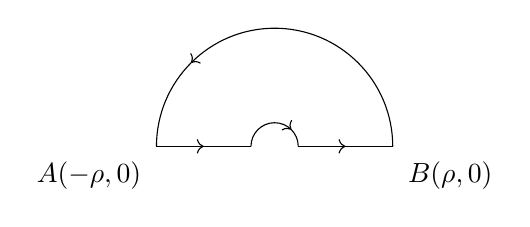
\begin{tikzpicture}[baseline=(current bounding box.north)]
        % A clipped circle is drawn
        \begin{scope}
            \draw [
            decoration={markings, mark=at position 0.75 with {\arrow{>}}},
            postaction={decorate}
            ](-0.3,0) arc[start angle=180, end angle=0, radius=0.3];
            \draw [
            decoration={markings, mark=at position 0.75 with {\arrow{>}}},
            postaction={decorate}
            ](1.5,0) arc[start angle=0, end angle=180, radius=1.5];
            
            \draw[decoration={markings, mark=at position 0.5 with {\arrow{>}}},
            postaction={decorate}](-1.5,0) -- (-0.3,0);
            \draw[decoration={markings, mark=at position 0.5 with {\arrow{>}}},
            postaction={decorate}](0.3,0) -- (1.5,0);
        \end{scope}
        %
        %%Labels for the vertices are typeset.
        \node[below left= 1mm of {(-1.5,0)}] {$A(-\rho,0)$};
        \node[below right= 1mm of {(1.5,0)}] {$B(\rho,0)$};
        \end{tikzpicture}
\end{figure}

Applying residue theorem \ref{sec:5.5.1:The Residue Theorem} to  $ z^{2\alpha+1}R(z^2) $ and take limits we have 
\begin{equation*}
    \int_{-\infty}^\infty z^{2\alpha+1}R(z^2)\dd z=2\pi i\sum_{y>0}\Res_{x+iy}z^{2\alpha+1}R(z^2)
\end{equation*}


%! TEX root = lecture/Complex_Analysis

And 
\begin{equation*}
    \begin{aligned}
        \int_{-\infty}^\infty z^{2\alpha+1}R(z^2)\dd z&=\int_0^\infty z^{2\alpha+1}R(z^2)\dd z+\int_0^\infty(-z)^{2\alpha+1}R(z^2)\dd z\\
        &=(1-e^{2\alpha\pi i})(1-e^{2\alpha\pi i})\int_0^\infty z^{2\alpha+1}R(z^2)\dd z
    \end{aligned}
\end{equation*}
So  $ \dps\int_0^\infty x^\alpha R(x)=\frac{2}{1-e^{2\alpha \pi i}}\cdot 2\pi i\cdot\sum_{y>0}\Res_{x+iy}z^{2\alpha+1}R(z^2) $.

\begin{example}
    Compute  $ \dps\int_0^\infty\frac{x^{\frac{1}{2}}}{1+x^2}\dd x $.
    
    
\begin{equation*}
    \begin{aligned}
        \int_0^\infty\frac{x^{\frac{1}{2}}}{1+x^2}\dd x=2\int_0^\infty\frac{t^2}{1+t^4}=\int_{-\infty}^\infty\frac{t^2}{1+t^4}\dd t
    \end{aligned}
\end{equation*}

Take  $ f(z)=\dps\frac{z^2}{1+z^4} $ and apply Residue Theorem \ref{sec:5.5.1:The Residue Theorem} to  $ f $, we have 
\[\int_{-\infty}^\infty \frac{t^2}{1+t^4}=\int_{-\infty}^\infty f(z)\dd z=2\pi i \sum_{y>0}\Res_{x+yi}f(z)=2\pi i[\Res_{\exp(\frac{i\pi   }{4})}f+\Res_{\exp(\frac{3i\pi}{4})}f]=\frac{\sqrt{2}\pi }{2}\] 
\end{example}

\subsection{Harmonic Functions}
\subsubsection{Definition and basis  properties}

A real-valued function  $ u(z)=u(x,y) $  in a region  $ \Omega  $ is \name{harmonic} if it is in $ C^2 $ and satisfying the Laplace's equation
\begin{equation}
    \triangle u=\frac{\partial^2 u }{\partial x^2}+\frac{\partial^2 u}{\partial y^2}=0\label{Laplace's equation}
\end{equation}

We already know that if  $ f(z)=u(x,y)+iv(x,y) $ is analytic in  $ \Omega  $, then  $ u $ and  $ v  $ satisfy the Cauchy-Riemann equations, and are therefore harmonic in  $ \Omega $.

If  $ u  $ is harmonic in  $ \Omega  $, then  $ f(z)=\dps\frac{\partial u}{\partial x}-i\frac{\partial u}{\partial y} $ is analytic in  $ \Omega $. This is because, for  $ U:=\dps\frac{\partial u}{\partial x}, V=-\frac{\partial u}{\partial y}$.
\begin{equation}\label{eq:5.6.1:harmonic function induces an anlytic function}
    \begin{cases}
        \dps\frac{\partial U }{\partial x}=\frac{\partial ^2 u}{\partial x^2}=-\frac{\partial ^2 u}{\partial y^2}=\frac{\partial V}{\partial y}\\
        \\
        
        \dps\frac{\partial U}{\partial y}=\frac{\partial ^2 u}{\partial x\partial y}=\frac{\partial ^2 u}{\partial y\partial x}=\frac{\partial V}{\partial x}
    \end{cases}
\end{equation}

We may write the differential 
\begin{equation}
    f \dd z=\left(\frac{\partial u}{\partial x}-i\frac{\partial u}{\partial y}\right)\left(\dd x+i\dd z\right)=\left(\frac{\partial u}{\partial x}\dd x+\frac{\partial u}{\partial y}\dd y \right)+i\left(\frac{\partial u }{\partial x}\dd y-\frac{\partial u }{\partial y }\dd x\right)\label{eq:5.6.1:differential of f}
\end{equation}

In this expression, the real part is  $ \dps\dd u=\frac{\partial u }{\partial x}\dd x+\frac{\partial u }{\partial y}\dd y $.
And if  $ u  $ has a conjugate harmonic function  $ v $, then the imaginary part is  \[\dps \dd v=\frac{\partial v }{\partial x}\dd x+\frac{\partial v}{\partial y}\dd y=-\frac{\partial u}{\partial y}\dd x+\frac{\partial u}{\partial x}\dd y  \]

In general, however, there is no (single-valued) conjugate function. We thus define 
\begin{equation}
    {}^*\dd u:=-\frac{\partial u}{\partial y}\dd x+\frac{\partial u}{\partial x}\dd y\label{eq:5.6.1:definition of conjugate differential of du}
\end{equation}
and call  $ {}^*\dd u  $ the \name{conjugate  differential of  $ \dd u $}. We may write \eqref{eq:5.6.1:differential of f} as 
\begin{equation}
    f\dd z=\dd u+i{}^*\dd u\label{eq:5.6.1:simplication of differential of f}
\end{equation}

\begin{lemma}\label{lemma:5.6.1:closed integral of *du is zero}
    Let  $ \gamma     $ be a cycle in a region  $ \Omega  $ \st  $ \gamma\sim 0 \mod \Omega$. Then 
    \begin{equation}
        \int_\gamma {}^*\dd u=0
    \end{equation} 
\end{lemma}
\begin{proof}
    \eqref{eq:5.6.1:simplication of differential of f} implies  $ \dps\int_\gamma f(z)\dd z=\int_\gamma\dd  u+i\int_\gamma {}^*\dd u $.
    
    Cauchy's Theorem \ref{General form of Cauchy's theorem} implies  $ \int_\gamma f(z)\dd z=0 $. And  $ \int_\gamma \dd u=0 $ since  $ \dd u  $ is an exact diffenrential. 
    
    Hence,  $ \int_\gamma {}^*\dd u=0 $.  
\end{proof}
\begin{theorem}\label{thm5.6.1:harmonic function is the real part of an analytic function in simply connected region}
    If  $ \Omega  $ is simply connected and  $ u  $ is harmonic in  $ \Omega  $, then  $ u  $ has a (single-valued) conjugate function  $ v  $ which uniquely determined up to additive constant.
\end{theorem}
\begin{proof}
    The last lemma \ref{lemma:5.6.1:closed integral of *du is zero} and theorem \ref{thm:5.1.2:integral conserved iff it is a derivative of an analytic function} imply that there is a (single-valued) function  $ v  $ \st  $ {}^*\dd u=\dd v $ \ie 
    \[\frac{\partial v}{\partial x}=-\frac{\partial u}{\partial x},\,\frac{\partial v}{\partial y}=\frac{\partial u}{\partial x}\] 

    So  $ v  $ is a conjugate function of  $ u $. (Notice that we use the property of simply connection that every cycle in  $ \Omega $ is homologous to zero)
    
    If  $ v_1  $ and  $ v_2  $ are two such harmonic functions, then  $ f_1=u+iv_1 $,  $ f_2=u+iv_2 $ are both analytic in  $ \Omega $. So  $ f_1-f_2=i(v_1-v_2) $ is analytic in  $ \Omega $. The open mapping theorem \ref{open mapping theorem} implies   $ f_1-f_2 $ is a constant. 
\end{proof}
\begin{remark}
    We see that the open mapping theorem \ref{open mapping theorem} has such power that it gives a way to prove an analytic function with some closed property is constant.
\end{remark}
\begin{remark}
    The condition on simply connectness can not be removed. For instance,  $ u(z)=\ln|z| $ is harmonic in  $ \Cbb\backslash\{0\} $, but it cannot be written as the real part of an analytic function since  $ \ln|z|=\mathrm{Re}\ln z $   
\end{remark}
\subsubsection{The Mean-value Property}

\begin{theorem}[Mean-value Property]\label{thm:5.6.2:mean-value property}
    Let  $ u  $ be harmonic in a region  $ \Omega  $. If  $ \overline{B(z,R)}\subset \Omega $, then 
    \begin{equation}
        u(z)=\int_0^{2\pi }u(z_0+Re^{i\theta})\dd \theta\label{eq:5.6.2:mean-value property}
    \end{equation} 
\end{theorem}
\begin{proof}
    The previous theorem \ref{thm5.6.1:harmonic function is the real part of an analytic function in simply connected region} implies that  $ u  $ has a conjugate function  $ v  $ on  $ \overline{B(z_0,R)} $. Consider the analytic function  $ f=u+iv $. The Cauchy integral formula \ref{Generalized version of Cauchy's integral formula}  shows 
    \begin{equation}
        f(z_0)=\frac{1}{2\pi i}\int_{|z-z_0|=R}\frac{f(z)}{z-z_0}\dd z=\frac{1 }{2\pi }\int_0^{2\pi }f(z_0+Re^{i\theta})\dd \theta
    \end{equation}
    This theorem follows by taking the real part of the equation.
\end{proof}
\begin{theorem}\label{thm:5.6.2:equation of mean value  property for more general harmonic function in a cirque}
    If  $ u  $ is harmonic in  $ \Omega $, and  $ \{z\in\Cbb:0<R_1 \leq |z-z_0| \leq R_2\}\subset \Omega $, then 
    \begin{equation}
        \frac{1 }{2\pi }\int_0^{2\pi }u(z_0+re^{i\theta})\dd\theta=\alpha\ln r+\beta\,r\in [R_1,R_2]
    \end{equation}  
    where  $ \alpha $ and  $ \beta $ are constants  
\end{theorem}
\begin{proof}
    In polar coordinate  $ (r,\theta) $,  \[ \dps\triangle=\frac{\partial^2 }{\partial r^2}+\frac{1}{r}\cdot\frac{\partial }{\partial r} +\frac{1}{r^2}\cdot\frac{\partial^2 }{\partial \theta^2}=r^{-1}\frac{\partial }{\partial r}(r\cdot\frac{\partial }{\partial r})+r^{-2}\frac{\partial ^2}{\partial \theta^2}\]

    Let  $ U(r)=\int_0^{2\pi }u(z_0+re^{i\theta})\dd\theta $.  $ z\mapsto u(z_0+z) $ is harmonic. Then 
    \begin{equation}
        \triangle U(r)=\frac{1}{2\pi }\int_0^{2\pi }\triangle u(z_0+re^{i\theta})\dd \theta=0
    \end{equation} 
    Therefore,  $ \dps\frac{\partial }{\partial r}\left(r\frac{\partial U}{\partial r}\right)=0 $. Therefore,
     $ U(r)=\alpha\ln \gamma+\beta $.  
\end{proof}
\begin{theorem}[Maximal Principle of Harmonic Function]\label{thm:5.6.2:maximal principle of harmonic function}
    A nonconstant harmonic function has neither a maximum nor a minimum in its region of definition.
\end{theorem}
\begin{proof}
    Suppose  $ u  $ attains a maximum at  $ z_0\in\Omega  $.  $ \exists R>0  $ \st  $ B(z_0,R)\subset \Omega $. Suppose  $ \exists a\in B(z_0,R) $ \st  $ u(a)<u(z_0)=M $.
    
    The mean-value property implies 
    \[M=u(z_0)=\frac{1}{2\pi }\int_0^{2\pi}u(z_0+re^{i\theta})\dd\theta<M \]
    by continuity. This causes a contradiction.
    
    So  $ u  $ is a constant in  $ B(z_0,R) $. 
    
    Then for every  $ z_1 $ in the region, since we can find a series of disk such that the center of the disk is in the previous disk and  $ z_0 $ is the center of the first disk,  $ z_1 $ is in the last disk.
    
    Then by the property above,  $ u(z_0)=u(z_1) $. So  $ u  $ is a constant, which causes a contradiction! 
\end{proof}

%! TEX root = lecture/Complex_Analysis

\begin{theorem}\label{thm:5.6.2:maximal principle of harmonic function on closed subset}
    $ u $ is harmonic in the interior  of  $ E $ and continuous on  $ \overline{E} $, which is bounded, then the maximum  and minimum of  $ u  $ are taken on  $ \partial E  $.
\end{theorem}
\begin{proof}
    It is followed from Theorem \ref{thm:5.6.2:maximal principle of harmonic function}
\end{proof}
It follows that the maximal norm of harmonic function $ u  $ is taken on  $ \partial E $, which implies a corollary 
\begin{corollary}\label{cor:5.6.2:u1=u2 iff u1=u2 on the boundary}
    If  $ u_1 $ and  $ u_2  $ are continuous on a closed bounded set  $ E  $ which are harmonic in the interior of  $ E  $ and  $ u_1=u_2  $ on the boundary of  $ E  $, then  $ u_1=u_2  $ on $ E  $.
\end{corollary}
\begin{proof}
    Apply the maximum and minimum principle to  $ u_1-u_2 $ 
\end{proof}
\subsubsection{Poisson's Formula}
\begin{theorem}[Poisson's formula]\label{thm:5.6.3:Poisson's formula}
    Suppose that  $ u  $ is harmonic on  $ B(0,R ) $ and continuous on  $ \overline{B(0,R)} $. Then 
    \begin{equation}
        u(a)=\frac{1 }{2\pi }\int_{|z|=R}\dps\frac{R^2-|a|^2}{|z-a|^2}u(z)\dd \theta\label{eq:5.6.3:Poisson's formula}
    \end{equation}
    for  $\forall  a\in B(0,R) $. 
\end{theorem}
\begin{proof}
    The idea is to use M{\"o}bius transformation and apply mean-value property.

    Let  $ \zeta=S^{-1}(z)=\dps\frac{\frac{z}{R}-\frac{a}{R}}{1-\frac{\bar{a}}{R}\cdot \frac{z}{R}}=\frac{R(z-a)}{R^2-\bar{a}\cdot z} $. So  $ \dps z=S(\zeta)=\frac{R(R\zeta+a)}{R+\bar{a}\zeta} $ is a M{\"o}bius transformation mapping the unit circle into  $ B(0,R) $ in which $ 0\mapsto a $.
    
    Suppose  $ u(S(\zeta)) $ is harmonic on  $ |\zeta| \leq 1 $(See Remark \ref{rmk:5.6.3:general case in the proof of Poisson's formula}). The mean-value property implies 
    \begin{equation}\label{eq1:5.6.3:Poisson's formula}
        \begin{aligned}
            u(S(0))=u(a)&=\dps\frac{-i}{2\pi}\int_{|\zeta|=1}u(\zeta)\frac{\dd\zeta}{\zeta}
        \end{aligned}
    \end{equation} 
    where
    \begin{equation}\label{eq2:5.6.3:Poisson's formula}
        \begin{aligned}
            \frac{\dd \zeta}{\zeta}&=\frac{R^2-\bar{a}z}{R(z-a)}\cdot\frac{R(R^2-|a|^2)}{(R^2-\bar{a}z)^2}\dd z\\
            &=\left[\frac{1}{z-a}+\frac{\bar{a}}{R^2-\bar{a}z}\right]\dd z\\
            &\overset{z=Re^{i\theta}}{=}\left[\dps\frac{iz}{z-a}+\frac{i\bar{a}z}{R^2-\bar{a}z}\right]\dd \theta\\
            &=\overset{R^2=z\bar{z}}{=}\left[\dps\frac{iz}{z-a}+\frac{i\bar{a}}{\bar{z}-\bar{a}}\right]\dd\theta\\
            &=i\frac{R^2-a^2}{|z-a|^2}\dd\theta
        \end{aligned}
    \end{equation}
    Combined with \eqref{eq1:5.6.3:Poisson's formula} and \eqref{eq2:5.6.3:Poisson's formula}, we obtain \eqref{eq:5.6.3:Poisson's formula} in a stronger assumption. 
    \[u(a)=\frac{1}{2\pi}\int_{|z|=R}\frac{R^2-|a|^2}{|z-a|^2}u(z)\dd \theta\]
\end{proof}

\begin{remark}
    Note that  
    \begin{equation}
        \begin{aligned}
            \dps\frac{R^2-|a|^2}{|z-a|^2}&=\dps\frac{z}{z-a}+\frac{\bar{a}}{\bar{z}-\bar{a}}\\
            &=\frac{1}{2}\left[\frac{z}{z-a}+\frac{\bar{a}}{\bar{z}-\bar{a}}+\frac{\bar{z}}{\bar{z}-\bar{a}}+\frac{a}{z-a}\right]\\
            &=\frac{1}{2}\left(\frac{z+a}{z-a}+\frac{\bar{z}+\bar{a}}{\bar{z}-\bar{a}}\right)\\
            &=\Real\left(\frac{z+a}{z-a}\right)
        \end{aligned}
    \end{equation}
    So the Poisson's formula can also be written as 
    \begin{equation}
        u(a)=\frac{1}{2\pi }\int_{|z|=R}\Real\left(\frac{z+a}{z-a}\right)u(z)\dd \theta,\,\forall a\in B(0,R)\label{eq':5.6.3:another form of Poisson's formula}
    \end{equation}
    or 
    \begin{equation}
        u(a)=\Real\left[\frac{1}{2\pi i}\dps\int_{|z|=R}\frac{z+a}{z-a}\cdot\frac{u(z)}{z}\dd z\right],\,\forall a\in B(0,R)\label{eq:5.6.3:Schwarz Formula}
    \end{equation}
    By Lemma \ref{sec5.2.3:Lemma of Analytic Properties of integral function},  $ u  $ is the real part of the analytic function 
    \[f(z)=\frac{1}{2\pi i}\int_{|\zeta|=R}\frac{\zeta+z}{\zeta-z}\cdot\frac{u(\zeta)}{\zeta}\dd \zeta+iC\]
    where  $ C\in\Rbb $. \eqref{eq:5.6.3:Schwarz Formula} is called the \name{Schwarz Formula}.
\end{remark}
\begin{remark}\label{rmk:5.6.3:general case in the proof of Poisson's formula}
    For the general assumption in the theorem \ref{thm:5.6.3:Poisson's formula}, note that if  $ r\in (0,1) $, then  $ u(rz) $ is harmonic in  $ \overline{B(0,R)} $. The above proof implies 
    \begin{equation}
        u(ra)=\frac{1}{2\pi}\int_{|z|=R}\frac{R^2-|a|^2}{|z-a|^2}u(rz)\dd\theta\label{eq3:5.6.3:Poisson's formula}
    \end{equation} 
    Since   $ u $ is continuous on a compact set  $ \overline{B(0,R)} $, it is uniformly continuous. Then $ u(rz)\rightrightarrows u(z) $ uniformly for  $ |z|=R $ as  $ r\rightarrow 1 $.
    
    Then take  $ r\rightarrow 0 $ in \eqref{eq3:5.6.3:Poisson's formula} and we obtain Poisson's formula  holds under the assumption of the theorem.
\end{remark} 
\subsubsection{Schwarz's Theorem}
We can easily define harmonic function $ u $ in the interior if  $ u  $ is piecewise continuous on the boundary by \eqref{eq:5.6.3:Schwarz Formula}. However, it is not always continuous at the boundary. The next theorem gives a condition that such an extended function $ u $ exists if  $ u  $ is continuous on the boundary.  
\begin{theorem}[Schwarz's theorem]\label{thm:5.6.4:Schwarz's theorem}
    Given a piecewise continuous function  $ u  $ on  $ [0,2\pi] $, the \name{Poisson integral }
    \begin{equation}
        P_u(z)=\frac{1}{2\pi }\int_0^{2\pi}\Real\left(\frac{e^{i\theta}+z}{e^{i\theta}-z}\right)u(\theta)\dd\theta
    \end{equation} 
    is harmonic for  $ |z|<1 $. Moreover,  $ \dps\lim_{\substack{\,\,\,z\to e^{i\theta}\\|z|<1}} P_u(z)=u(\theta_0)$  if  $ u $ is continuous t  $ \theta_0 $.   
\end{theorem}
\begin{proof}
    Lemma \ref{sec5.2.3:Lemma of Analytic Properties of integral function} implies  $ P_u $ is harmonic in  $ |z|<1 $.  

    Note that  $ P  $ is a \textbf{linear functional} which maps piecewise continuous function  $ u  $ on  $ [0,2\pi] $ to harmonic function  $ P_u $ on the unit disk. Explicitly,
    \begin{equation}\label{eq1:5.6.4:Schwarz's theorem}
        \begin{cases}
            P_{u_1+u_2}=P_{u_1}+P_{u_2} \\
            P_{\lambda u}= \lambda P_u
        \end{cases}
    \end{equation}

    Applying Poisson's formula \ref{thm:5.6.3:Poisson's formula} to  $ u\equiv 1 $, we get  $ P_1=1 $, and thus  $ P_c=c ,\forall c\in \Rbb$.   

    If  $ u \geq 0 $ on  $ [0,2\pi] $, then  $ P_u \geq 0 $. \eqref{eq1:5.6.4:Schwarz's theorem} follows that if  $ -\infty<m \leq u(\theta) \leq M<\infty $ for  $ \forall \theta\in [0,2\pi] $, then  $ m \leq P_u \leq M $. 
    
    By replacing  $ u $ with  $ u-u(\theta_0) $, WLOG, we may assume  $ u(\theta_0)=0 $.
    
    If $ u  $ is continuous at  $ \theta_0 $, then  $ \forall \epsilon>0 $, one can choose  $ C_2\subset \partial B(0,1) $ \st  $ e^{i\theta_0}\in\mathrm{int}(C_2) $ and  $ |u(\theta) |<\frac{\epsilon}{2}$ for  $ \forall e^{i\theta}\in C_2 $. Let  $ C_1=\partial B(0,1)\setminus C_2 $. Define
    \begin{align}
        u_1(\theta)=\begin{cases}
            u(\theta),&e^{i\theta}\in C_1\\
            0,&\text{otherwise}
        \end{cases}
        \quad
        &u_2(\theta)=\begin{cases}
            u(\theta),&e^{i\theta}\in C_2\\
            0,&\text{otherwise}
        \end{cases}
    \end{align}  

    Linearity of  $ P $ implies  $ P_u=P_{u_1}+P_{u_2} $.  $ \dps|u_2|<\frac{\epsilon}{2} $ $ \Rightarrow |P_{u_1}(z)|<\frac{\epsilon}{2},\forall z\in B(0,1) $. So  $ \dps \lim_{\substack{\,\,\,z\to e^{i\theta}\\|z|<1}} P_{u_2}(z)=0 $ 
    
     $ P_{u_1} $ can be viewed as a line integral over  $ C_1 $  $ \Rightarrow $  $ P_{u_1} $ is harmonic in  $ \Cbb\setminus C_1 $. So  $ P_{u_1} $ is harmonic in  $ \Cbb\setminus C_1 $ by lemma \ref{sec5.2.3:Lemma of Analytic Properties of integral function}.

    $ \dps\Real\left(\frac{e^{i\theta}+z}{e^{i\theta}-z}\right)=\frac{1-|z|^2}{|z-e^{i\theta}|^2} $  $ \Rightarrow  $  $ P_{u_1}(z)=0 $ for  $ z\in C_2 $. Continuity  implies  $ \dps \lim_{\substack{\,\,\,z\to e^{i\theta}\\|z|<1}} P_{u_1}(z)=0$.

    Therefore,  $ \dps \lim_{\substack{\,\,\,z\to e^{i\theta}\\|z|<1}} P_{u}(z)=0=u(\theta_0) $ 
\end{proof}
\subsubsection{The Reflection Principle}
\begin{theorem}[The reflection principle]\label{thm:5.6.5:The reflection principle}
    Let  $ \Omega  $ be a region which is symmetric w.r.t. the  $ x $-axis, and  $ \Omega^+:=\Omega\cap\{z\in \Cbb:\Imag z>0\} $,  $ \sigma=\Omega\cap\{z\in \Cbb:\Imag z=0\} $. Suppose that  $  v  $ is continuous in  $ \Omega^+\cup\sigma $, harmonic on  $ \Omega^+ $, and  zero on  $ \sigma $. Them  $ v  $ has a harmonic extension to  $ \Omega $, which satisfies  $ v(\bar{z})=-v(z) $. In the same situation, if   $ v  $ is the imaginary part of an analytic function  $ f(z) $ in  $ \Omega^+ $, then  $ f(z)  $ has an analytic extension  which satisfies  $ f(z)=\overline{f(\bar{z})} $. 
\end{theorem}

% TEX root = lecture/Complex_Analysis 

\begin{center}
    \tikzset{every picture/.style={line width=0.75pt}} %set default line width to 0.75pt        
    
    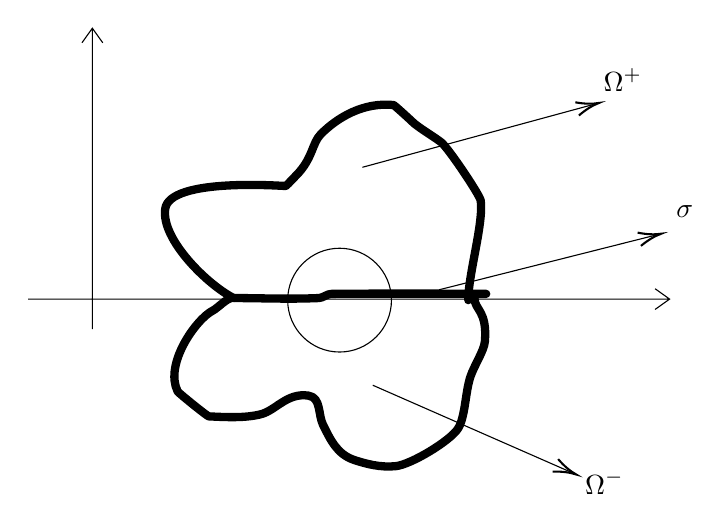
\begin{tikzpicture}[x=0.75pt,y=0.75pt,yscale=-1,xscale=1]
    %uncomment if require: \path (0,392); %set diagram left start at 0, and has height of 392
    
    %Shape: Axis 2D [id:dp13575276746597464] 
    \draw  (175,195.5) -- (484,195.5)(205.9,65) -- (205.9,210) (477,190.5) -- (484,195.5) -- (477,200.5) (200.9,72) -- (205.9,65) -- (210.9,72)  ;
    %Shape: Free Drawing [id:dp14268765045810194] 
    \draw  [line width=3] [line join = round][line cap = round] (274,195) .. controls (261.8,188.9) and (238.88,166.87) .. (241,152) .. controls (243.17,136.83) and (297.23,141.04) .. (299,141) .. controls (299.35,140.99) and (303.48,136.52) .. (304,136) .. controls (312.16,127.84) and (311.69,120.31) .. (316,116) .. controls (324.02,107.98) and (336.42,100.54) .. (351,102) .. controls (351.37,102.04) and (359.04,109.04) .. (360,110) .. controls (362.76,112.76) and (370.64,117.31) .. (374,120) .. controls (377.49,122.8) and (392.64,145.49) .. (393,148) .. controls (394.51,158.55) and (387,183.78) .. (387,196) ;
    %Shape: Free Drawing [id:dp6374095064796427] 
    \draw  [line width=3] [line join = round][line cap = round] (273,195) .. controls (270.83,195) and (265.99,200) .. (264,201) .. controls (256,205) and (240.39,226.79) .. (247,240) .. controls (247.33,240.66) and (261.29,251.97) .. (262,252) .. controls (270.19,252.39) and (279.33,252.92) .. (287,251) .. controls (294.33,249.17) and (299.56,240.51) .. (310,242) .. controls (316.15,242.88) and (314.61,251.22) .. (317,256) .. controls (320.53,263.06) and (323.66,270.22) .. (332,273) .. controls (337.54,274.85) and (344.62,276.74) .. (352,276) .. controls (359.28,275.27) and (377.97,264.05) .. (382,258) .. controls (385.56,252.65) and (385.57,240.3) .. (388,233) .. controls (389.83,227.5) and (394.64,220.34) .. (395,216) .. controls (396.26,200.86) and (390,200.83) .. (390,195) ;
    %Shape: Circle [id:dp9197077331741318] 
    \draw   (300,196) .. controls (300,182.19) and (311.19,171) .. (325,171) .. controls (338.81,171) and (350,182.19) .. (350,196) .. controls (350,209.81) and (338.81,221) .. (325,221) .. controls (311.19,221) and (300,209.81) .. (300,196) -- cycle ;
    %Straight Lines [id:da8903842986356113] 
    \draw    (336,132) -- (448.07,101.52) ;
    \draw [shift={(450,101)}, rotate = 164.79] [color={rgb, 255:red, 0; green, 0; blue, 0 }  ][line width=0.75]    (10.93,-3.29) .. controls (6.95,-1.4) and (3.31,-0.3) .. (0,0) .. controls (3.31,0.3) and (6.95,1.4) .. (10.93,3.29)   ;
    %Straight Lines [id:da4166743347978691] 
    \draw    (341,237) -- (437.17,279.2) ;
    \draw [shift={(439,280)}, rotate = 203.69] [color={rgb, 255:red, 0; green, 0; blue, 0 }  ][line width=0.75]    (10.93,-3.29) .. controls (6.95,-1.4) and (3.31,-0.3) .. (0,0) .. controls (3.31,0.3) and (6.95,1.4) .. (10.93,3.29)   ;
    %Shape: Free Drawing [id:dp9885674880852715] 
    \draw  [line width=3] [line join = round][line cap = round] (274,195) .. controls (287.22,195) and (299.93,195.63) .. (315,195) .. controls (317.11,194.91) and (318.89,193.03) .. (321,193) .. controls (344.33,192.68) and (414.33,193) .. (391,193) ;
    %Straight Lines [id:da3473062677735872] 
    \draw    (373,191) -- (478.06,164.49) ;
    \draw [shift={(480,164)}, rotate = 165.84] [color={rgb, 255:red, 0; green, 0; blue, 0 }  ][line width=0.75]    (10.93,-3.29) .. controls (6.95,-1.4) and (3.31,-0.3) .. (0,0) .. controls (3.31,0.3) and (6.95,1.4) .. (10.93,3.29)   ;
    
    % Text Node
    \draw (451,83) node [anchor=north west][inner sep=0.75pt]   [align=left] {$\displaystyle \Omega ^{+}$};
    % Text Node
    \draw (442,277) node [anchor=north west][inner sep=0.75pt]   [align=left] {$\displaystyle \Omega ^{-}$};
    % Text Node
    \draw (486,149) node [anchor=north west][inner sep=0.75pt]   [align=left] {$\displaystyle \sigma $};
    
    
    \end{tikzpicture}
\end{center}
\begin{proof}
    
    $ h(z)=\begin{cases}
        v(z),&z\in \Omega^+\\
        0,&z\in\sigma\\
        v(\bar{z}),&z\in\Omega^-
    \end{cases} $.

    We need to prove that  $ h $ is harmonic in  $ \Omega $. It suffices to prove  $ h  $ is harmonic on  $ \sigma $. Choose  $ \daleth  $ small \st  $ \overline{B(x,\delta)}\subset \Omega $. Let  $ P_h  $ be the Poisson integral  w.r.t.  $ \partial B(x_0,\delta) $ with the boundary values  $ h  $.

    Schwarz' theorem \ref{thm:5.6.4:Schwarz's theorem} implies  $ P_h $ is harmonic in  $ \overline{B(x,\delta)} $ and continuous on  $ \overline{B(x_0,\delta)} $. It follows that,
    
    (1) $ v-P_h $ is harmonic in the upper half disk  $ B(x_0,\delta)\cap\{z\in\Cbb:\Imag z>0\} $. 

    (2) $ v-P_h=0 $ on  $ \partial B(x,\delta)\cap\{z\in\Cbb:\Imag z \geq 0\} $.  

    $ \forall x\in B(x_0,\delta\cap )\sigma $, apply Poisson formula \ref{eq:5.6.3:Poisson's formula}
    \begin{equation}
        P_h(x)=\frac{1}{2\pi}\int_0^{2\pi}\dps\frac{\delta^2-|x|^2}{|\delta e^{i\theta}-x|^2}h(\delta e^{i\theta})\dd\theta=0
    \end{equation} 
    by symmetry.

    Apply the maximum and  minimum principle \ref{cor:5.6.2:u1=u2 iff u1=u2 on the boundary} to  $ h-P_h $, we get  $ h=P_h $ in  $ B(x,\delta)\cap\{z\in \Cbb:\Imag z \geq 0\} $.
    
    The same argument works for the lower half disk.

    So  $ h=P_h  $ in  $ B(x_0,\delta) $ $ \Rightarrow  $  $ h  $ is harmonic at  $ x_0 $.
    
    For the second part of the theorem, it is enough to prove  $ \tilde{f}(z)=\begin{cases}
        f(z),&z\in\Omega^+\\
        \overline{f(\bar{z})},&z\in\Omega^-
    \end{cases} $ 
    is analytic on  $ \sigma $.
    
    For  $ \forall x_0\in\sigma $, let  $ B(x_0,\delta) $ be as before. We already proved  $ v  $ can be extended to a harmonic function in  $ B(x_0,\delta) $.  $ v  $ has a conjugate function  $ -u_0 $ iin the same disk. We may normalize  $ u_0  $ \st  $ u_0=\Real f(z) $  in  $ B(x_0,\delta\cap\{z\in\Cbb,\Imag z>0\}) $. Define  $ g(z):=u_0(z)-u_0(\bar{z}) $.
    
    Then  $ g(x)=0 $ for  $ x\in B(x_0,\delta)\cap \sigma $ $ \Rightarrow  $ 
    \begin{align*}
        \frac{\partial g}{\partial x}(z)=0,\,\forall z\in B(x_0,\delta)\cap\sigma\\
        \frac{\partial g}{\partial y}(x)=2\frac{\partial u_0}{\partial y}(z)=-2\frac{\partial v}{\partial x}(z)=0
    \end{align*}  

    So the analytic function  $ \dps\frac{\partial g}{\partial x}-i\frac{\partial g}{\partial y}\equiv 0 $ on   $ B(x,\delta)\cap \sigma $.(It is analytic because of \eqref{eq:5.6.1:harmonic function induces an anlytic function}) Then  $ \dps\frac{\partial g}{\partial x}-i\frac{\partial g}{\partial y}\equiv 0 $  in  $ B(x_0,\delta) $ $ \Rightarrow  $   $ g\equiv 0 $.
    
    So  $ u_0(z)=u_0(\bar{z}) $,  $ \forall z\in B(x_0,\delta) $  $ \Rightarrow  $  $ f(z)=u_0(z)+i v(z) $ is analytic in  $ B(x_0,\delta) $ and  $ f(z)=\overline{f(\bar{z})} $ for  $ \forall z\in B(x_0,\delta) $.



\end{proof}

\section{Series and Product Representations}
\subsection{Power Series Expansions}
\subsubsection{Weierstrass's Theorem}
\begin{theorem}[Weierstrass's Theorem]\label{thm:5.1.1:Weierstrass's Theorem}
    Suppose  $ f_n  $ is analytic in the region  $ \Omega_n  $ for each  $ n\in \Nbb  $, and  $ \Omega_1\subset \Omega_2\subset\cdots\subset\Omega_n\subset\cdots $ and  $ \dps\bigcup_{n\in \Nbb}\Omega_n=\Omega $. If  $ f_n  $ converges to  $ f  $ in  $ \Omega  $, uniformly on every compact subset of  $ \Omega  $, then  $ f $ is analytic in  $ \Omega  $. 

    Moreover,  $ f_n' $ converges uniformly to  $ f' $ on every compact subset of  $ \Omega $.  
\end{theorem}
\begin{proof}
    $ \forall  $ compact subset  $ K\subset \Omega  $,  $ K\subset\dps \bigcup\limits_{n=1}^\infty \Omega_n$ $ \Rightarrow $   $ \exists N\in \Nbb $ such that  $ K\subset \dps\bigcup_{n=1}^{N}\Omega_n $.

    $ \forall z_0\in \Omega $,  $ \exists   R>0 $ \st  $ \overline{B(z_0,R)}\subset \Omega $. Choose  $ N\in \Nbb $ \st  $ \overline{B(z_0,R)}\subset \Omega_n $ for  $ \forall n \geq N $.
    
    Cauchy's integral formula \ref{General form of Cauchy's theorem} implies 
    \begin{equation}
        f_n(z)=\frac{1}{2\pi i}\int_{\partial B(z_0,R)}\frac{f_n(\zeta)}{\zeta-z}\dd\zeta,\,\forall z\in B(z_0,R)
    \end{equation}

    $ f_n\rightrightarrows f  $ uniformly on  $ \overline{B(z_0,R)} $  $ \Rightarrow  $ 
    \begin{equation}
        f(z)=\frac{1}{2\pi i}\int_{\partial B(z_0,R)}\frac{f(\zeta)}{\zeta-z}\dd\zeta
    \end{equation} 
    Then  $ f  $ is  analytic in  $ B(z_0,R)$ by lemma \ref{sec5.2.3:Lemma of Analytic Properties of integral function}.

    \begin{equation}
        \begin{cases}
            f_n'(z)=\dps\frac{1}{2\pi i}\int_{\partial B(z_0,R)}\frac{f_n(\zeta)}{(\zeta-z)^2}\dd\zeta&\forall z\in B(z_0,R)\\
            f'(z)=\dps\frac{1}{2\pi i}\int_{\partial B(z_0,R)}\frac{f(\zeta)}{(\zeta-z)^2}\dd\zeta&\forall z\in B(z_0,R)
        \end{cases}
    \end{equation}
    Then  $ |f_n'(z)-f'(z)| \leq\dps \frac{1}{2\pi}\int_{\partial B(z_0,R)}\dps\frac{|f_n(\zeta)-f(\zeta)|}{|\zeta-z|^2}|\dd\zeta| $. Therefore,  $ f_n'  $ uniformly converges to  $ f' $ in  $ B(z_0,\rho ) $ for  $ 0<\rho<R$.    

    Since any compact subset of  $ \Omega  $ can be covered by a finite number of such closed disks,  $ f_n\rightrightarrows f$ uniformly on every compact subset of  $ \Omega  $.
\end{proof}
\begin{corollary}\label{cor:5.1.1:Corollary of Weierstrass's Theorem}
    If  $ f_n  $ is analytic in a region  $ \Omega  $ for  $ n\in \Nbb  $, and  $ \dps\sum_{j=1}^n f_j\rightrightarrows f $ on every compact subset of  $ \Omega $, then  $ f  $ is analytic  in  $ \Omega  $ and $ f'(z)=\dps\sum_{j=1}^\infty f_j'(z),\,\forall z\in \Omega $ uniformly on every compact subset of  $ \Omega $.
\end{corollary}
\begin{theorem}[Hurwitz's Theorem]\label{thm:5.1.1:Hurwitz's Theorem}
    If the functions  $ f_n  $ are analytic and nowhere zero in a region  $ \Omega  $, and if  $ f_n\rightrightarrows f $ on every compact subset of  $ \Omega $, then  $ f  $ is either identically zero or never equal to  $ 0  $ in  $ \Omega $.    
\end{theorem}
\begin{proof}
    Suppose  $  f \not\equiv 0 $. The zeros of  $ f  $ are isolated.

     $ \forall z_0\in \Omega  $,  $ \exists \delta>0  $ \st  $ f(z)\neq 0 $,  $ \forall z\in B(z_0,\delta)\setminus \{z_0\}\subset\Omega $.
     
     Then  $ |f|  $ has a positive minimum on  $ \partial B(z_0,\delta) $. Thus, $ \dps\frac{1}{f_n}\rightrightarrows \frac{1}{f} $ on  $ \partial B(z_0,\delta) $.
     
    Combined with $ f_n'\rightrightarrows f' $ on  $ \partial B(z_0,\delta) $  $ \Rightarrow $
    \begin{equation}
        \lim_{n\to\infty}\frac{1}{2\pi i}\int_{\partial B(z_0,\delta)}\frac{f_n'(z)}{f_n(z)}\dd z=\frac{1}{2\pi i}\int_{\partial B(z_0,\delta)}\frac{f'(z)}{f(z)}\dd z
    \end{equation}  
    By argument principle \ref{The Argument Principle}, this equation equals to  $ 0 $. So  $ f  $ has no zeros on  $ \partial B(z_0,\delta) $, so is on  $ \Omega $. 
\end{proof}

\subsubsection{The Taylor Series}
\begin{theorem}\label{thm:5.1.2:Theorem of Taylor Series}
    If  $ f  $ is analytic in the region  $ \Omega  $, and  $ z_0\in \Omega  $, then the expression 
    \begin{equation}
        f(z)=\sum_{n=0}^\infty \frac{f^{(n)}(z_0)}{n!}(z-z_0)^n
    \end{equation}
    is valid in the largest open disk of  $ z_0 $ contained in   $ \Omega  $.
\end{theorem}
\begin{proof}
    Taylor's theorem \ref{Taylor's Theorem} implies 
    \begin{equation}
        f(z)=f(z_0)+f'(z_0)(z-z_0)+\cdots+\frac{f^{(n)}(z_0)}{n!}(z-z_0)^n+f_{n+1}(z)(z-z_0)^{n+1},\,
    \end{equation}
    for  $ \forall z\in B(z_0,R)\subset \overline{B(z_0,R)}\subset \Omega $, where  
    \begin{equation}
        f_{n+1}(z)=\dps\frac{1}{2\pi i}\int_{\partial B(z_0,R)}\frac{f(\zeta)}{(\zeta-z)^{n+1}(\zeta-z)}\dd\zeta 
    \end{equation}
    Let  $ M:=\dps\max_{z\in\partial B(z_0,R)}|f(z)| $. Then  $ |f_{n+1}(z)(z-z_0)^{n+1}|<\dps\frac{M}{R^n(R-|z-z_0|)}\cdot |z-z_0|^{n+1}\rightrightarrows 0$ in every disk  $ |z-z_0| \leq \rho<R $, from which we derive this theorem.
\end{proof}


Some known Taylor series:
\begin{equation}
    \begin{aligned}\label{eq:5.1.2Taylor Series of some functions}
        e^z&=1+z+\frac{z^2}{2!}+\cdots+\frac{z^n}{n!}+\cdots,\quad z\in \Cbb\\
        \cos z&=1-\frac{z^2}{2!}+\frac{z^4}{4!}-\cdots+\frac{(-1)^n z^{2n}}{(2n)!}+\cdots,\quad z\in \Cbb\\
        \sin z &= z-\frac{z^3}{3!}+\frac{z^5}{5!}-\cdots+\frac{(-1)^n z^{2n+1}}{(2n+1)!}+\cdots,\quad z\in \Cbb\\
        \ln  (1+z)&=z-\frac{z^2}{2}+\frac{z^3}{3}-\cdots+(-1)^{n+1}\frac{z^n}{n}+\cdots,\quad \forall |z|<1\\
        \forall \mu\in \Rbb\setminus\Zbb_{\geq 0},(1+z)^{\mu}&=1+\mu z+\binom{\mu}{2}z^2+\cdots+\binom{\mu }{n}z^n+\cdots,\quad \forall |z|<1
    \end{aligned}
\end{equation}
where  $ \dps\binom{\mu }{n}=\frac{\mu (\mu -1)\cdots(\mu -n+1)}{n!} $, and pick the branch with  $ \ln 1=0 $.

\subsubsection{Laurent Series}
\begin{lemma}
    Let  $ A:=\{z\in\Cbb:R_1<|z-a|<R_2\} $ be an annulus. For each analytic function  $ f:A\rightarrow \Cbb  $, there are analytic functions  $ f_1:\{z\in\Cbb:|z-a|<R_2\}\rightarrow \Cbb  $,  $ f_2:\{z\in \Cbb:|z-a|>R_1\}\rightarrow \Cbb $ \st  $ f(z)=f_1(z)+f_2(z),\,\forall z\in A $    
\end{lemma}
\begin{proof}
    For  $ \forall z\in A  $,  $ f_1(z)=\dps\frac{1}{2\pi i}\int_{|\zeta-a|=r_1}\frac{f(\zeta)}{\zeta-z}\dd \zeta $,  $ r_1\in (|z-a|,R_2) $.  

    Cauchy's theorem \ref{General form of Cauchy's theorem} implies the integral is independent of the choice of  $ r_1$. 

    If we fix such  $ r  $, then  $ f_1(z)  $ is analytic for  $ \forall |z-a|<r_1 $.  $ \overset{r_1\to R_2}{\Rightarrow}  $ $ f_1(z)  $ is well-defined and   analytic on  $ B(a,R_2) $.

    Let  
    \begin{equation}
        f_2(z)=-\dps\frac{1 }{2\pi i}\int_{|\zeta-a|=r_2}\frac{f(\zeta)}{\zeta-z}\dd\zeta,\,r_2\in(R_1,|z-a|)\label{eq:5.1.2:f_2 in lemma}
    \end{equation}
    Then  $ f_2  $ is well-defined and analytic in  $ \{z\in\Cbb:|z-a|>R_1\} $.  

    Denote $ \gamma_1=\{z:|z-a|=r_1\} $,  $ \gamma_2=\{z:|z-a|=r_2\} $,  $ R_1<r_2<|z-a|<r_1<R_1 $.
    
    Cauchy's integral formula \ref{Generalized version of Cauchy's integral formula} implies  
    \begin{equation}
        f(z)=n(\gamma_1-\gamma_2,z)f(z)=\dps\frac{1}{2\pi i}\int_{\gamma_1-\gamma_2}\frac{f(\zeta)}{\zeta-z}\dd \zeta=f_1(z)+f_2(z),
        \,\forall z\in A
    \end{equation}
\end{proof}
\begin{theorem}[Laurent Theorem]\label{thm:5.1.3:Laurent Theorem}
    Any analytic function  $ f  $ on  $ A=\{z\in \Cbb:R_1<|z-a|<R_2\} $ has a power series of the form 
    \begin{equation}
        f(z)=\sum_{n=-\infty}^\infty c_n(z-a)^n\label{eq:5.1.3:Laurent Series}
    \end{equation} 
    This series, called \name{Laurent series}, converges uniformly on each compact subset of  $ A  $. Moreover, 
    \begin{equation}
        c_n=\frac{1 }{2\pi i}\int_{|\zeta-a|=r}\frac{f(\zeta)}{(\zeta-a)^{n+1}}\dd\zeta,\,\forall n\in \Zbb,\,\forall r\in (R_1,R_2)
    \end{equation}
\end{theorem}
\begin{proof}
    The previous lemma implies  $ f(z)=f_1(z)+f_2(z),\,\forall z\in A $, where  $ f_1  $ is analytic in  $ |z-a|<R_2 $ and  $ f_2  $ is analytic in  $ |z-a|>R_1 $. Then Taylor series for  $ f_1  $ is
    \begin{equation}
        f_1(z)=\sum_{n=0}^\infty a_n(z-a)^n
    \end{equation}
    which converges uniformly on each compact subset of  $ |z-a|<R_2 $.
    
    Let  $ g(z)=f_2(a+\dps\frac{1}{z}) $,  $ |z|<\dps\frac{1}{R_1} $. \eqref{eq:5.1.2:f_2 in lemma} tells us  $ \dps\lim_{z\to\infty}f_2(z)=0 $. Then  $ \dps\lim_{z\to 0}g(z)=0 $ $ \Rightarrow  $  $ g $ can be viewed as an analytic function in  $ B(0,\dps\frac{1}{R_1}) $.

    The Taylor's series for  $ g  $ is  $ g(z)=\dps\sum_{n=1}^\infty b_nz^n  $, which converges uniformly on each compact subset of  $ B(0,\dps\frac{1}{R_1}) $. Now let  $ \zeta=a+\frac{1}{z} $. Then 
    \begin{equation}
        f_2(\zeta)=g(z)=g(\frac{1}{\zeta-a})=\sum_{n=1}^\infty b_n (\zeta-a)^n
    \end{equation} 
    which converges uniformly on each compact subset  $ |z-a|>R_1 $.  
    \begin{equation}
        f(z)=\sum_{n=-\infty}^\infty c_n(z-a)^n
    \end{equation}
    which converges uniformly on each compact subset of  $ A $. Then
    \begin{equation}
        \frac{1}{2\pi i}\int_{|z-a|=r}\frac{f(z)}{(z-a)^{n+1}}\dd z =\frac{1}{2\pi i}\sum_{k=-\infty}^\infty c_k\sum_{|z-a|=r}(z-a)^{k-(m+1)}\dd z,\,\forall z\in (R_1,R_2)
    \end{equation}
    where  $ \dps\int_{|z-a|=r}(z-a)^{k-(n+1)}\dd z\neq 0 $ iff  $ k=n $.  So 
    \begin{equation}
        c_n=\frac{1 }{2\pi i}\int_{|\zeta-a|=r}\frac{f(\zeta)}{(\zeta-a)^{n+1}}\dd\zeta,\,\forall n\in \Zbb,\,\forall r\in (R_1,R_2)
    \end{equation}
\end{proof}
\begin{theorem}
    Let  $ f  $ be analytic in  $ \Omega\setminus\{a\} $, where  $ \Omega  $ is a region and  $ a  $ is an isolated singularity. Its Laurent series is given by  $ f(z)=\dps\sum_{n=-\infty}^\infty c_n(z-a)^n $, $ \forall z\in B(a,R)\setminus\{a\}\subset \Omega\setminus\{a\} $. Then 
    \begin{enumerate}
        \item [(a)]  $ f  $ has a removable singularity at  $ a  $ iff  $ c_n =0 $ for  $ n<0 $   
        \item [(b)]  $ f  $ has a pole of order  $ N $ at  $ a $ iff  $ c_n=0 $ for  $ n<-N $ and  $ c_{-N}\neq 0 $.
        \item [(c)]  $ f  $ has an essential singularity at  $ a $ iff   $ c_n\neq 0 $ for infinitely many negative  $ n $.
    \end{enumerate}  
\end{theorem}
\begin{proof}
    (a) and (b) can be derived from the explicit expression of  $ f_1,f_2 $.
    
    For (c), "$ \Rightarrow $" follows from (b) and (a).

    "$ \Leftarrow $" follows from the fact that isolated singularities belong to one of three categories: removable singularities, poles, and essential singularities, \ie theorem \ref{thm:4.3.2:Classification of isolated singularities}.
\end{proof}
\subsection{Partial Fractions and Factorization}
\subsubsection{Partial fractions}
\begin{theorem}[Mittag-Leffler Theorem]\label{thm:5.2.1:Mittag-Leffler Theorem}
    Let  $ \{\zeta_k:k\in \Nbb\} $ be a sequence in  $ \Cbb  $,  $ \dps\lim_{k\to\infty}\zeta_k=\infty $, and let  $ P_k  $ be polynomials without constant term. Then there are functions which are meromorphic in  $ \Cbb  $ with poles at just the points  $ \zeta_k $ and the corresponding singular part  $ P_k\left(\dps\frac{1}{z-\zeta_k}\right) $. Moreover, the most general meromorphic function of this kind can be written as
    \begin{equation}
        \label{eq:5.2.1:Mittag-Leffler Theorem}
        f(z)=\sum_{k}\left[P_{k}\left(\frac{1}{z-\zeta_k}\right)-p_k(z)\right]+g(z)
    \end{equation}
    where  $ p_k  $ are polynomials and  $ g $ is entire. 
\end{theorem}


% !TEX root = lecture/Complex_Analysis

\begin{proof}
    WLOG, we assume  $ \zeta_k\neq0  $ for each  $ k  $. Consider the Taylor expansion for  $ P_k(\dps\frac{1}{z-\zeta_k}) $ around  $ z=0 $:
    \begin{equation}
        \Psi(z)=P_k(\frac{1}{z-\zeta_k})=\Psi(0)+\Psi'(0)z+\dps\frac{\Psi''(0)}{2!}z^2+\cdots+\frac{\Psi^{(N_k)(0)}}{N_k!}z^{N_k}+\Psi_{N_k+1}z^{N_k+1}
    \end{equation}  
    where  $ N_k  $ is to be specified later, and 
    \begin{equation}
        \Psi_{N_k+1}(z)=\frac{1}{2\pi i}\int_C\frac{\Psi(\zeta)}{\zeta^{N_k+1}(\zeta-z)}\dd\zeta
    \end{equation}
    where  $ C  $ is the circle centered at  $ 0 $ with radius  $ \dps\frac{|\zeta_k |}{2} $. Let  $ M_k:\dps\max_{z\in C}|\Psi(z)| $. Then 
    \begin{equation}
        |\Psi_{N_k+1}(z)| \leq \frac{1}{2\pi }\frac{M_k}{\left(\dps\frac{|\zeta_k|}{2}   \right)^{N_k+1}\cdot\dps \frac{|\zeta_k|}{4}}\cdot 2\pi \cdot\frac{|\zeta_k|}{4}=2M_k\left(\dps\frac{2}{|\zeta_k|}\right)^{N_k+1},\,\forall z\text{ with }|z| \leq \frac{|\zeta_k|}{4}
    \end{equation}

    Let  $ p_k $ be the partial sum of  $ \Psi  $ up to   $ z^{N_k} $.\ie  $ p_k=\Psi(0)+\Psi'(0)z+\dps\frac{\Psi''(0)}{2!}z^2+\cdots+\frac{\Psi^{(N_k)(0)}}{N_k!}z^{N_k} $.  Then 
    \begin{equation}
        |\Psi(z)-p_k(z)|  \leq 2 M_k\left(\frac{2|z|}{|\zeta_k|}\right)^{N_k+1},\,\forall z \text{ with }|z| \leq \frac{|\zeta_k|}{4}
    \end{equation}  
    Pick  $ N_k  $ large enough \st  $ M_k\cdot 2^k \leq 2^{N_k } $. Then
    \begin{equation}\label{eq2:5.2.1:Mittag-Leffler Theorem}
        |\Psi(z)-p_k(z)| \leq 2^{-k}\Rightarrow |P_k(\dps\frac{1}{z-\zeta_k})-p_k(z)| \leq 2^{-k},\,\forall z \text{ with }|z| \leq \frac{|\zeta_k|}{4}
    \end{equation}
    Note that 
    \begin{equation*}
        \sum_k\left[P_k(\frac{1}{z-\zeta_k})-p_k(z)\right]=\sum_{|\frac{\zeta_k}{4}| \leq R}\left[P_k(\frac{1}{z-\zeta_k})-p_k(z)\right]+\sum_{|\frac{\zeta_k}{4}|>R}\left[P_k(\frac{1}{z-\zeta_k})-p_k(z)\right]
    \end{equation*}
    where the first part is a finite sum and has  $ \dps P_k(\frac{1}{z-\zeta_k}) $ as the singular part at the pole  $ \zeta_k $, and the second part
    is analytic in  $ z\in \overline{B(0,R)} $ by Weierstrass's theorem \ref{Weierstrass Theorem for Essential singularity} and \eqref{eq2:5.2.1:Mittag-Leffler Theorem}  

    Therefore,  $ h(z)=\dps \sum_k\left[P_k(\frac{1}{z-\zeta_k})-p_k(z)\right]$ is the desired meromorphic function.

    For the second part, if  $ f  $ is meromorphic in  $ \Cbb  $ with the some poles  $ \zeta_k  $ and singular parts as  $ h  $, then 
     $ g=f-h  $ is analytic in  $ \Cbb $. 
\end{proof}
\begin{remark}
    We have given  $ p_k $ as the partial sum of  $ \dps P_k(\frac{1}{z-\zeta_k}) $ up to some  $ N_k $   
\end{remark}
\begin{example}
    Prove that 
    \begin{equation}\label{pi^2/sin^2piz}
        \frac{\pi^2}{\sin^2(\pi z)}=\sum_{n=-\infty}^\infty\frac{1}{(z-n)^2}    
    \end{equation}
\end{example}
\begin{proof}
    The singular part of  $ \dps\frac{\pi^2}{\sin^2(\pi z)} $ at the pole  $ z=0 $ is  $ \dps\frac{1}{z^2} $ $ \Rightarrow  $ The singular part
    of  $ \dps\frac{\pi^2}{\sin^2(\pi z)} $    at  $ z=n\in\Zbb $ is  $ \dps\frac{1}{(z-n)^2}$. We know  $ \dps\sum_{n=-\infty}^\infty\frac{1}{(z-n)^2} $
    converges uniformly on each compact set in  $ \Cbb  $ if we omit the terms which become infinite (\ie  $ p_k =0 $ in the previous theorem)
    
    The Mittag-Leffler Theorem \ref{thm:5.2.1:Mittag-Leffler Theorem} implies  $ \dps\frac{\pi^2}{\sin^2(\pi z)}=\dps\sum_{-\infty}^\infty \frac{1}{(z-n)^2}+g(z) $ 
    where  $ g  $ is analytic in  $ \Cbb $.
    
    It is easy to see that  $  g  $ has period  $ 1  $ and  $ \dps\lim_{|y|\to\infty}g(x+iy)=0 $ uniformly in  $ x\in \Rbb $.
    
    Then  $ |g(z)| $ is bounded in  $ \{z\in \Cbb:0 \leq \Re z \leq 1\} $ $ \Rightarrow  $  $ |g(z) $ is bounded in  $ \Cbb $ by its periodicity.
    
    Then Liouville's theorem \ref{Liouville's Theorem} implies  $ g  $ is a constant, hence of  $ 0  $ since  $ \dps\lim_{y\to\infty}g(x+iy)=0 $. 
\end{proof}
Similarly, one can prove 
\begin{equation}\label{pi cotpi}
    \pi\cot(\pi z)=\frac{1}{z}+\sum_{n\neq 0}\frac{1}{z-n}+\frac{1}{n}=\frac{1}{z}+\sum_{n=1}^\infty\frac{2z}{z^2-n^2},\,z\in \Cbb
\end{equation}

From  \eqref{pi^2/sin^2piz} and \eqref{pi cotpi}, one can derive 
\begin{equation}
    \frac{\pi}{\sin(\pi z)}=\lim_{m\to\infty}\sum_{n=-m}^m\frac{(-1)^n}{z-n},\,z\in\Cbb
\end{equation}
\subsubsection{Infinite Products}
An \name{infinite product} of complex numbers  $ \dps\prod_{n=1}^\infty a_n $ converges if and only if at most a finite number of the factors are zero,
and if the partial products formed by the non-vanishing factors tend to a finite limit which is different from zero. 

\begin{remark}
     $ \dps\prod_{n=1}^\infty a_n$ converges  $ \Rightarrow  $   $ a_n=\dps\frac{\dps\prod_{j=1}^n a_j}{\dps\prod_{j=1}^{n-1}a_j}\rightarrow 1 $ as 
      $ n\rightarrow \infty  $ (if the zero factors are omitted)  
\end{remark}
\begin{theorem}\label{thm:5.2.2:equivalence of convergence of products}
    The infinite product  $ \dps\prod_{n=1}^\infty (1+a_n) $ with  $ 1+a_n\neq 0 $ converges if and only if  $ \dps\sum_{n=1}^\infty \mathrm{Ln}(1+a_n) $
    converges, where  $ \mathrm{Ln} $ is the principal branch of the logarithm.    
\end{theorem}
\begin{proof}
    "$ \Leftarrow $": Let  $ S_n =\dps\sum_{k=1}^n\mathrm{Ln}(1+a_k) $. Then  $ P_n=\dps \prod_{k=1}^n(1+a_k)=e^{S_n} $.
    
    So  $ s_n\rightarrow s $ as  $ n\rightarrow \infty $ $ \Rightarrow  $  $ P_n\rightarrow P=e^s\neq 0 $ as  $ n\rightarrow\infty $    

    "$ \Rightarrow $" Suppose  $ P_n\rightarrow P\neq 0 $ as  $ n\rightarrow \infty $.
    
    There exists  $ M_n\in \Zbb $ \st  $ \dps\mathrm{Ln}(\frac{P_n}{P})=S_n-\mathrm{Ln}P+2\pi i \cdot M_n$,  $ n\in \Nbb $.
    
    Then  $ 2\pi (M_{n+1}-M_n)=\dps\arg(\frac{P_{n+1}}{P})-\arg(\frac{P_n}{P})-\arg(1+a_{n+1}) $. From  $ \dps\lim_{k\to\infty}\frac{P_n}{P}=1 $
    we can derive  $ \dps\arg(\frac{P_{n+1}}{P})-\arg(\frac{P_{n}}{P})\rightarrow 0 $ as  $ n\rightarrow \infty $.
    
    $ |\arg(1+a_{n+1})| \leq \pi $ $ \Rightarrow  $  $ M_{n+1}-M_n=0 $ for  $ n  $ large enough. So  $ M_n=M\in\Zbb $ for all large  $ n $.
    
    Then  $ \mathrm{Ln}(\dps\frac{P_n}{P})=S_n-\mathrm{Ln} P+2\pi i\cdot M $, $ n\in \Nbb $ $ \Rightarrow  $  $ S_n\rightarrow \mathrm{Ln}P-2\pi i \cdot M $
    as  $ n\rightarrow \infty $    
\end{proof}

The infinite product  $ \dps\prod_{n=1}^\infty(1+a_n) $ is said to be \subname{absolutely convergent}{infinite product} if the infinite sum  $ \dps\sum_{n=1}^\infty \mathrm{Ln}(1+a_n) $ 
is absolutely convergent.
\begin{theorem}\label{thm:5.2.2:equivalence of product absolutely convergence}
    The product  $ \dps\prod_{n=1}^\infty (1+a_n)  $ is absolutely convergent iff  $ \dps\sum_{n=1}^\infty |a_n| $ converges. 
\end{theorem} 
\begin{proof}
    Convergence of either  $ \dps\sum_{n=1}^\infty\mathrm{Ln}(1+a_n) $ or  $\dps \sum_{n=1}^\infty|a_n| $ implies  $ a_n\rightarrow 0 $ as  $ n\rightarrow \infty  $ 
    
     $ \dps\lim_{z\to 0}\frac{\mathrm{Ln}(1+z)}{z}=0 $ $ \Rightarrow  $  $ \dps\frac{1}{2}|a_n|<|\dps\mathrm{Ln}(1+a_n)|<\frac{3}{2}|a_n| $ for all large  $ n $.   
\end{proof}





\subsubsection{Canonical Products}
If  $ g  $ is an entire function, then  $ f(z)=e^{g(z)} $ is entire and everywhere nonzero. Conversely, if  $ f  $ is any entire function which is never zero, then  $ g(z)=\ln f(z)  $ is well-defined. So  $ f(z)=e^{g(z)} $ where  $ g  $ is entire. 

This result gives a way to construct the most general function with a finite number of zeros. Assume  $ f  $ has a zero of order  $ m  $ at the origin, and  $ N  $ zeros  $ a_1,\cdots,a_N $ away from the origin.(multiple zeros being repeated) Then 
\begin{equation}
    f(z)=z^me^{g(z)}\prod_{n=1}^N(1-\dps\frac{z}{a_n})\label{eq:5.2.3:function with finite zeros}
\end{equation}
where  $ g  $ is entire.

If there are infinitely many zeros, an obvious generalization is 
\begin{equation}
    f(z)=z^me^{g(z)}\prod_{n=1}^\infty(1-\dps\frac{z}{a_n})\label{eq:5.2.4:function with infinite zeros}
\end{equation}
Theorem \ref{thm:5.2.2:equivalence of product absolutely convergence} implies  $ \dps\prod_{n=1}^\infty (1-\frac{z}{a_n}) $ converges absolutely iff  $ \dps\sum_{n=1}^\infty\frac{1}{|a_n|} $ converges. And in this   case, the convergence is also uniform in  $ \{z:|z| \leq R\} $ for  $ \forall R>0 $.

\begin{theorem}[Weierstrass factorization theorem]\label{thm:5.2.3:Weierstrass factorization theorem}
    There exists an entire function with arbitrary prescribed zeros $ (a_n)_{n\in \Nbb} $ as long as  $ a_n\rightarrow \infty $ if the number of zeros is infinite.  Moreover, every entire function with these and no other zeros can be written as 
    \begin{equation}
        f(z)=z^me^{g(z)}\prod_{n=1}^\infty(1-\dps\frac{z}{a_n})\exp\left[\frac{z}{a_n}+\frac{1}{2}(\frac{z}{a_n})+\cdots+\frac{1}{N_n}(\frac{z}{a_n})^{N_n}\right]
    \end{equation}
    where the product is taken over all  $ a_0\neq 0 $,  $ N_n \in \Nbb\cup\{0\} $, and  $ g  $ is entire. 
\end{theorem}
\begin{proof}
    We already proved the case when the number of zeros is finite in   \eqref{eq:5.2.3:function with finite zeros}. So we consider a sequence of complex numbers  $ a_n\neq 0 $ with  $ \dps\lim_{n\to\infty}a_n=\infty $. We need to prove that  $ \exists  $ polynomials  $ p_n(z) $ \st   $ \dps\prod_{n=1}^\infty(1-\frac{z}{a_n}e^{p_n(z)}) $ converges to an entire function. By theorem \ref{thm:5.2.2:equivalence of convergence of products}, this is equivalent to the uniform convergence of 
    \begin{equation}
        \sum_{n=1}^\infty[\ln(1-\frac{z}{a_n})+p_n(z)]
    \end{equation}  
    where the branch of the logarithm shall be chosen \st  $\dps r_n(z)=\ln(1-\frac{z}{a_n})+p_n(z) $ has imaginary part in  $ (-\pi,\pi] $.
    
    For given  $ R>0  $, we only need to consider the terms with  $ |a_n|>R $.

    The Taylor series gives 
    \begin{equation}
        \Ln(1-\frac{z}{a_n})=-\left[\frac{z}{a_n}+\frac{1}{2}(\frac{z}{a_n})^2+\cdots\right],\,|z| \leq R
    \end{equation}
    We define  $ \dps p_n(z)=\frac{z}{a_n}+\frac{1}{2}\left(\frac{z}{a_n}\right)^2+\cdots+\frac{1}{N_n}\left(\frac{z}{a_n}\right)^{N_n} $, where  $ N_n\in \Nbb\cup\{0\} $ is to be specified later. 
    

    Then  \[ r_n\left(z\right)=\dps-\left[\frac{1}{N_n+1}\left(\frac{z}{a_n}\right)^{N_n+1}+\frac{1}{N_n+2}\left(\frac{z}{a_n}\right)^{N_n+2}+\cdots\right]+2k_n\pi,\, |z| \leq R ,k_n\in \Zbb\]
    
    And thus   
    \begin{align*}
        \dps|r_n\left(z\right)| &\leq \frac{1}{N_n+1}\left(\frac{z}{|a_n|}\right)^{N_n+1}\cdot\left[1+\frac{R}{|a_n|}+\left(\frac{R}{|a_n|}\right)^2+\cdots\right]\\
        &=\frac{1}{N_n+1}\left(\frac{R}{|a_n|}\right)^{N_n+1}\left(1-\frac{R}{|a_n|}\right)^{-1},\,|z| \leq R 
    \end{align*}

    If we choose  $ N_n=n $, then  $ r_n(z)\rightarrow 0 $ as  $ n\rightarrow\infty $. Then  $ \Imag (r_n(z))\in(-\pi,\pi] $ for all large  $ n $. So  $ k_n=0 $ for enough large  $ n $.  
    Moreover,  $ \sum r_n(z) $ is absolutely and uniformly convergent for  $ |z| \leq R $.
    
    So  $ \dps\prod_{n=1}^\infty(1-\frac{z}{a_n})e^{p_n(z)} $ is analytic in  $ B(0,R) $ for  $ \forall R>0 $.    
\end{proof}

\begin{corollary}
    Every function which is meromorphic in  $ \Cbb  $ is the quotient of two entire functions.
\end{corollary}
\begin{proof}
    If  $ F  $ is meromorphic in  $ \Cbb  $, the theorem \ref{thm:5.2.3:Weierstrass factorization theorem} implies that we can construct an entire function  $ g  $ whose zeros are the poles of  $ F $. Then  $ f(z)=F(z)g(z) $. So  $ F(z)=\dps\frac{f(z)}{g(z)} $ 
\end{proof}

The proof of the  Weierstrass factorization theorem \ref{thm:5.2.3:Weierstrass factorization theorem} tells us  
\begin{equation}
    \prod_{n=1}^\infty(1-\frac{z}{a_n})\exp\left[\frac{z}{a_n}+\frac{1}{2}\left(\frac{z}{a_n}\right)^2+\cdots+\frac{1}{h}\left(\frac{z}{a_n}\right)^h\right]\label{eq:5.2.3:canonical product}
\end{equation}
converges and represents an entire function is  
\begin{equation}
    \frac{1}{n+1}\sum_{n=1}^\infty\left(\frac{R}{|a_n|}\right)^{h+1}
\end{equation}
converges for all  $ R>0 $ $ \Leftrightarrow $  $ \dps\sum_{n=1}^\infty\frac{1}{|a_n|^{h+1}} $ converges.

Suppose  $ h  $ is the smallest integer for which  $ \dps\sum_{n=1}^\infty \frac{1}{|a_n|^{h+1}} $ converges. For this  $ h  $, \eqref{eq:5.2.3:canonical product} is called the \name{canonical product} associated with the sequence  $ \{a_n\} $, and  $ h  $ is the \name{genus} of the canonical product.

If  $ f  $ has a Weierstrass factorization for which the infinite product is a canonical product, and if in this representation  $ g  $ reduces to a polynomial, then  $ f  $ is said to be of \name{finite genus}.
The \name{genus} of  $ f $ is then defined to be  \[\dps\max\{\text{degree of  $ g $ },\text{ genus of the canonical product}\} \]
\begin{example}
    An entire function of genus zero is of the form 
    \begin{equation}
        f(z)=Cz^m\prod_{n=1}^\infty(1-\frac{z}{a_n})
    \end{equation}
    with  $ C\in \Cbb\setminus\{0\} $, and  $ \dps\sum_{n=1}^\infty\frac{1}{|a_n|}<\infty $. 
\end{example}


\begin{example}
    The canonical representation of  an entire function of genus one is either of form 
    \begin{equation}
        f(z)=Cz^m e^{\alpha z}\prod_{n=1}^\infty(1-\frac{z}{a_n})\exp\left[\frac{z}{a_n}\right]
    \end{equation}
    with  $ C\in\Cbb\setminus\{0\},\dps\sum\frac{1}{|a_n|}=\infty,\sum_{n=1}^\infty\frac{1}{|a_n|^2}<\infty $,

    or of the form 
    \begin{equation}
        f(z)=Cz^m e^{\alpha z}\prod_{n=1}^\infty(1-\frac{z}{a_n})
    \end{equation}
    with  $ C\in\Cbb\setminus\{0\} $, $ \alpha\neq 0 $,  $ \dps\sum\frac{1}{|a_n|}<\infty $.   
\end{example}
\begin{example}
    Prove that  $ \sin(\pi z)=\pi z\dps\prod_{n=1}^\infty(1-\frac{z^2}{n^2}),\,\forall z\in \Cbb\setminus\Zbb $.\label{product expression of sin pi z}
\end{example}
\begin{proof}
    The zeros of  $ \sin(\pi z) $ are  $ z=n,\,n\in \Zbb $. The genus of the canonical product associated with  $ \{n\}_{n\in\Zbb_+} $ is one.
    
    So by Weierstrass factorization theorem \ref{thm:5.2.3:Weierstrass factorization theorem}, we must take  $ h=1 $, and 
    \begin{equation}
        \sin(\pi z)=z e^{g(z)}\prod_{n\neq 0}(1-\frac{z}{n})e^{\frac{z}{n}}
    \end{equation} 

    Taking logarithmic derivatives on both sides, we get 
    \begin{equation}
        \pi \cot(\pi z)=\frac{1}{z}+g'(z)+\sum_{n\neq 0}\left(\frac{1}{z-n}+\frac{1}{n}\right)
    \end{equation}
    uniformly converges on compact sets in  $ \Cbb\setminus\Zbb $.
    
    Comparing with the expression for  $ \pi \cot(\pi z) $ in \eqref{pi cotpi}, we obtain  $ g'(z)\equiv 0 $ and since
    $ \dps\lim_{z\to0} \frac{\sin(\pi z)}{z}=\pi $, we have 
    \begin{equation*}
        \sin \pi z=\pi z\prod_{n\neq 0}(1-\frac{z}{n})e^{\frac{z}{n}}=\pi z\prod_{n=1}^\infty (1-\frac{z^2}{n^2})
    \end{equation*}
    Here we use the absolute convergence and uniform convergence of the product.
\end{proof}

\subsubsection{The Gamma Function}
\begin{equation}
    \name{$ \Gamma(z) $}=\int_0^\infty t^{z-1}e^{-t}\dd t,\,\Re z>0
\end{equation}

%! TEX root = lecture/Complex_Analysis

Let  $ f_n(z)=\dps\int_0^n t^{z-1}e^{-t}\dd t $. Then  $ f_n(z)  $ is analytic in  $ \Re z>0 $ and 
\begin{equation}
    |f_n(z)-\Gamma(z)|=|\int_n^\infty t^{z-1}e^{-t}\dd t| \leq \int_n^\infty t^{\Re z-1}e^{-t}\dd t
\end{equation}  
which converges uniformly in  $ \{z\in \Cbb:\delta \leq \Re z \leq M\} $ for  $ \forall \delta>0,M>0 $. By Weierstrass' theorem \ref{thm:5.1.1:Weierstrass's Theorem},  $ \Gamma  $  is analytic in  $ \{z:\Re z>0\} $.

\begin{proposition}\label{thm:5.2.4:properties of the Gamma function}
    Here are some properties of the Gamma function:
    \begin{enumerate}[label=(\alph*)]
        \item $ \Gamma(z+1)=z\Gamma(z) $,  $ \forall z\in \Cbb\setminus\{0,-1,\cdots,\} $. In particular,  $ \Gamma(n+1)=n! $,  $ \forall n\in \Nbb $.
        
        \item  $ \Gamma  $ extends to a meromorphic function on   $ \Cbb  $ with simple poles at  $ z=0,-1,-2,\cdots, $
        
        \item  $ \dps\frac{1}{\Gamma(z)}=z e^{\gamma z}\dps\prod_{n=1}^\infty (1+\frac{z}{n})e^{-\frac{z}{n}} $,  $ z\in \Cbb $, where  $ \dps\gamma=\lim_{n\to\infty}\sum_{k=1}^n\frac{1}{k}-\ln n  $ is the Euler's constant 
        
        \item  $ \Gamma(z)=\dps\lim_{n\to\infty}\frac{n!n^z}{z(z+1)\cdots(z+n)} $,  $ \forall z\in \Cbb\setminus\{0,-1,-2,\cdots\} $.
        
        \item  $ \Gamma  $  has no zeros,  $ \dps\frac{1}{\Gamma} $ is entire.
        
        \item  $ \Gamma(z)\Gamma(1-z)=\dps\frac{\pi}{\sin(\pi z)}  $,  $ \forall z\in \Cbb\setminus\Zbb $  
    \end{enumerate}
\end{proposition}

\begin{proof}
    \,


    \begin{enumerate}[label=(\alph*)]
        \item Integration by parts  $ \Rightarrow  $  $ \Gamma(z+1)=z\Gamma(z) $,  $ \Re z>0 $.
        \item We use  $ \Gamma(z+1)=z\Gamma(z) $ to analytically continue  $ \Gamma  $ to meromorphic function on  $ \Cbb $.
        Then 
        \begin{equation}
            \Gamma_1(z)=\frac{\Gamma(z+1)}{z}
        \end{equation}
        is analytic on  $ \{z\in \Cbb:\Re z>-1\}\setminus\{0\} $ \st  $ \Gamma_1(z)=\Gamma(z) $ for  $ \Re z>0 $.
        
        $ z=0 $  is a simple pole of  $ \Gamma_1 $ with  $ \Res_{z>0}\Gamma_1(z)=\Gamma(1)=1 $.
        
        By induction, if we have  $ \Gamma_{n-1} $ as the analytic continuous of  $ \Gamma $ to  $ \Re z>1-n $,  $ z\neq -n+2,-n+3,\cdots,0 $, then we define 
        \begin{equation}
            \Gamma_n(z)=\frac{\Gamma_{n-1}(z+1)}{z}=\frac{\Gamma(z+n)}{z(z+1)\cdots(z+n-1)}
        \end{equation}
        which is meromorphic for  $ \Re z>-n $.with poles  $ z=-n+1,,-n+2\cdots,0 $ and  $ \dps\Res_{z=-n+1}\Re\Gamma_n(z)=\frac{(-1)^{n-1}}{(n+1)!} $. 

        \item[(c,d,e)] We know that  $ \dps\lim_{n\to\infty}(1-\dps\frac{t}{n})^nt^{z-1}=e^{-t}t^{z-1} $, and   $ (1-\dps\frac{t}{n})^n \leq e^{-t} $ for  $ 1 \leq t \leq n $.
        
        Then dominated convergence theorem implies  \[ \dps\lim_{n\to\infty}\int_0^n(1-\dps\frac{t}{n})^n t^{z-1}\dd t=\int_0^\infty e^{-t}t^{z-1}\dd  t=\Gamma(z),\forall \Re z>0\]

        \begin{claim}
            \begin{equation}\label{eq:5.5.3:lim of equation in Gamma function}
                \int_0^n(1-\dps\frac{t}{n})^nt^{z-1}\dd t=\frac{n!n^z}{z(z+1)\cdots(z+n)},\,\Re z>0
            \end{equation}
        \end{claim}
        \begin{proof}
            Indeed, for  $ n=1 $,  $ \dps\int_0^1(1-t)t^{z-1}\dd t=\frac{1}{z}-\frac{1}{z+1} $.  
        \end{proof}

        Suppose \eqref{eq:5.5.3:lim of equation in Gamma function} holds for  $ n-1 $. Then 
        \begin{equation}
            \begin{aligned}
                \int_0^n(1-\frac{t}{n})^nt^{z-1}\dd t&\overset{s=\frac{t}{n}}{=}n^z\int_0^1(1-s)^ns^{z-1}\dd s \\
                &=\frac{n^z}{z}\left[(1-s)^ns^z|^1_0+n\int_0^1(1-s)^{n-1}s^z\dd z\right]\\
                &=\frac{n^{z+1}}{z}\int_0^1(1-s)^{n-1}s^z\dd s\\
                &=\frac{n^{z+1}}{z}\cdots\frac{(n+1)!}{z(z+1)\cdots(z+n-1)}\text{ by induction hypothesis}\\
                &=\frac{n!n^z}{z(z+1\cdots(z+n))}
            \end{aligned}
        \end{equation} 
        Therefore,  $ \Gamma(z)=\dps\lim_{n\to\infty}\frac{n!n^z}{z(z+1)\cdots(z+n)} $,  $ \Re z>0 $.

        For  $ \Re z>0  $,  
        \begin{align}
            \dps\frac{1}{\Gamma(z)}&=\lim_{n\to\infty}\frac{z(z+1)\cdots(z+n)}{n!n^z}\notag\\
            &=z\lim_{n\to\infty}e^{-z\ln n}(1+z)(1+\dps\frac{z}{2})\cdots(1+\frac{z}{n})\notag\\
            &=z\lim_{n\to\infty}\exp\left[z\left(\sum_{k=1}^n\frac{1}{k}-\ln n\right)\right]\prod_{k=1}^n(1+\frac{z}{k})e^{-\frac{z}{k}}\notag\\
            &=ze^{\gamma z}\prod_{k=1}^n(1+\frac{z}{k})e^{-\frac{z}{k}}\label{eq:5.2.4:inverse of Gamma function}
        \end{align}
        
        Weierstrass factorization theorems implies that \eqref{eq:5.2.4:inverse of Gamma function} represents an entire function with zeros at  $ 0,-1,-2,\cdots $.
        
        Then the extension of  $ \Gamma(z) $ and  $ \dps\frac{1}{\Gamma(z)} $ should have those above properties (c), (d) and (e). 

        \item[(f)] For  $ \forall z\in \Cbb\setminus\Zbb $, we have 
        
        \begin{equation}
            \begin{aligned}
                \frac{1}{\Gamma(z)\Gamma(1-z)}&=-\frac{1}{z\Gamma(z)\Gamma(1-z)}\\
                &=-\frac{1}{z}\cdot z e^{\gamma z}\prod_{k=1}^\infty (1+\frac{z}{k})e^{-\frac{z}{k}}\cdot(-z)e^{-\gamma z}\prod_{k=1}^\infty(1-\frac{z}{k})e^{\frac{z}{k}}\\
                &=z\prod_{k=1}^\infty(1-\frac{z^2}{k^2})\\
                &\overset{\eqref{product expression of sin pi z}}{=}\frac{\sin \pi z}{\pi}
            \end{aligned}
        \end{equation} 
    \end{enumerate} 
\end{proof}

One may use (d) to prove 
\begin{equation}
    \sqrt{\pi}\Gamma(2z)=2^{2z-1}\Gamma(z)\Gamma(z+\frac{1}{2}),\,z\neq 0,-1,-2,\cdots,z\neq -\frac{1}{2},-\frac{3}{2},\cdots
\end{equation}
which is known as Legendre's duplication formula.

\subsection{Entire Functions}
\subsubsection{Jensen's formula}
\begin{theorem}[Jensen's formula]\label{thm:5.3.1:Jensen's formula}
    Suppose  $ f  $ is analytic in  $ |z| \leq \rho $, and all of its zeros in  $ |z|<\rho $ are  $ a_1,\cdots,a_n $ (multiple zeros being repeated) Assume  $ z=0  $ is not a zero. Then 
    \begin{equation}
        \ln |f(0)|=-\sum_{j=1}^n\ln\left(\frac{\rho}{|a_j|}\right)+\frac{1}{2\pi }\int_0^{2\pi}\ln|f(\rho e^{i\theta})|\dd\theta\label{eq:5.3.1:Jensen's formula}
    \end{equation}  
\end{theorem}
\begin{remark}
    \begin{enumerate}[label=(\arabic*)]
        \item Jensen's formula relates the modulus  $ |f(z)| $ on a circle to the modulus of the zero in the interior enclosed by the circle.
        \item If  $ f(0)=0 $, then  $ f(z)=Cz^k+\cdots $. We apply  \eqref{eq:5.3.1:Jensen's formula} to  $ f(z)\dps\left(\frac{\rho}{z}\right)^k $ and get 
        \begin{equation}
            \ln |c|+k\ln \rho=-\sum_{j=1}^n\ln\left(\frac{\rho}{|a_j|}\right)+\frac{1}{2\pi }\int_0^{2\pi}\ln|f(\rho e^{i\theta})|\dd\theta
        \end{equation}
    \end{enumerate}

\end{remark}
\begin{proof}
    We first assume that  $ f  $ is free of zeros in  $ |z| \leq \rho $. Then  $ \ln |f(z)|  $ is harmonic in  $ |z| \leq \rho $. Mean value property \ref{thm:5.6.2:mean-value property} implies  $ \ln|f(0)|=\dps\frac{1}{2\pi }\int_0^{2\pi} \ln |f(\rho e^{i\theta})| \dd\theta $. It remains valid if  $  f  $ has zeros on the circle  $ |z|=\rho $. We divide  $ f  $ with one factor  $ z-\rho e^{i\theta_0} $ for zeros  $ \rho e^{i\theta_0} $. It suffices to prove that 
    \[\ln \rho=\frac{1}{2\pi}\int_0^{2\pi}\ln|\rho e^{i\theta}-\rho e^{i\theta_0}|\dd\theta\]
    \[\Leftrightarrow\int_0^{2\pi}\ln|e^{i\theta}-e^{i\theta_0}|\dd\theta=0\Leftrightarrow\int_0^{2\pi}\ln|e^{i\theta}-1|\dd\theta=0\Leftrightarrow\int_0^{\pi}\ln\sin t\dd t=-\pi \ln 2\]
    
    Finally, for any  $ f  $ satisfying the assumption of the theorem, we know 
    \begin{equation}
        F(z)=f(z)\cdot\prod_{j=1}^n\frac{\rho^2-\bar{a}_jz}{\rho(z-a_j)}
    \end{equation}
    is free from zeros in the disk  $ |z|<\rho $, and  $ |F(z)|=|f(z)|  $ on  $ |z|=\rho $ $ \Rightarrow $
    \[\ln|F(0)|=\frac{1}{2\pi}\int_0^{2\pi}\ln|f(\rho e^{i\theta})|\dd\theta\]
    \[\Rightarrow \ln|f(0)|=-\sum_{j=1}^n\ln\left(\frac{\rho}{|a_j|}\right)+\frac{1}{2\pi}\int_0^{2\pi}\ln|f(\rho e^{i\theta})|\dd\theta\]  
\end{proof}
\begin{remark}
    Apply the Poisson formula \ref{thm:5.6.3:Poisson's formula} to  $ \ln|F(z)| $, we get the \name{Poisson-Jensen formula} 
    \begin{equation}\label{eq:5.3.1:Poisson-Jensen formula}
        \ln|f(z)|=-\sum_{j=1}^n\ln\left|\frac{\rho^2-\overline{a_j}z}{\rho(z-a_j)}\right|+\frac{1}{2\pi}\int_0^{2\pi}\Re\frac{\rho e^{i\theta}+z}{\rho e^{i\theta}-z}\ln|f(\rho e^{i\theta})|\dd\theta,\,\forall z\text{ with }|z|<\rho,f(z)\neq 0
    \end{equation}
\end{remark}

\subsubsection{Order of an entire function}
The \name{order}  of the entire function  $ f  $ is defined by 
\begin{equation}
    \lambda:=\limsup_{r\to\infty}\frac{\ln\ln M(r)}{\ln r}\,\text{ where }\,M(r):=\max_{|z|=r}|f(z)|
\end{equation}
In other words,  $ \lambda  $ is the smallest number \st 
\begin{equation}
    M(r) \leq \exp[r^{\lambda+\epsilon}]
\end{equation}
for  $ \forall \epsilon>0 $ as soon as  $ r $ large enough.

\begin{theorem}[Hadamard Theorem]\label{thm:5.3.2:Hadamard Theorem}
    The genus $ h $  and the order $ \lambda $  of an entire function satisfy the double inequality  $ h \leq \lambda \leq h+1 $. 
\end{theorem}
The proof is omitted now.


\section{Riemann Mapping Theorem}

\subsection{Normal families}
\subsubsection{The Arzela-Ascoli Theorem}
Let  $ \mathscr{F} $ be a family of functions  $ f  $, defined in a fixed region  $ \Omega\subset \Cbb $, with values in a metric space  $ S $. The distance function in  $ S  $ is denoted by  $ d $.

The functions in a family  $ \mathscr{F} $  are said to be \name{equicontinuous} on a set  $ E\subset \Omega $ if for  $ \forall \epsilon>0 $,  $ \exists \delta>0 $ \st  $ d(f(z),f(z_0))<\epsilon  $,  $ \forall z,z_0\in E $ with  $ |z-z_0|<\delta $ and  $ \forall f\in \mathscr{F} $.

\begin{remark}
    Each  $ f  $ in an equicontinuous family is itself uniformly continuous on  $ E $. 
\end{remark}

A family is said to be \name{normal} (or \name{relatively compact}) in  $ \Omega $ if every sequence  $ \{f_n\} $ of functions  $ f_n\in \mathscr{F} $ contains a subsequence which converges uniformly on every compact subset of  $ \Omega $.

\begin{remark}
    This definition does not require the limit functions of the convergent subsequences to be members of  $ \mathscr{F} $. 
\end{remark}
Let  $ E_k:=\Omega\cap \overline{B(0,k)}\cap \{z\in \Cbb:d(z,\partial \Omega) \geq \dps\frac{1}{k}\} $,  $ k\in \Nbb $.

Then  $ E_k  $ is bounded and closed, and hence compact.

$ \forall  $ compact set  $ E\subset \Omega  $ is bounded and has positive distance from  $ \partial \Omega $ $ \Rightarrow  $  $ E\subset E_k $. So the choice of  $ E_k  $ is representative.

Define  $ \delta(a,b)=\dps\frac{d(a,b)}{1+d(a,b)} $. It is easy to check that  $ \delta  $ is a metric and has the advantage of being bounded.

Define  \begin{equation}\label{eq:6.1.1:definition of delta_k in function space}
    \delta_k(f,g)=\dps\sup_{z\in E_k}\delta(f(z),g(z)) ,\,\rho(f,g)=\dps\sum_{k=1}^\infty\delta_k(f,g)2^{-k} 
\end{equation}

It is easy to check that  $ \rho(f,g) $ is finite and is a distance between  $ f $ and  $ g $ on  $ \Omega $.  

\begin{lemma}\label{thm:6.1.1:Lemma of Arzela-Ascoli Theorem}
     $ f_n\rightrightarrows f$ on every compact subset of  $ \Omega  $ if and only if  $ \rho(f_n,f)\rightarrow 0 $ as  $ n\rightarrow \infty $.    
\end{lemma}
\begin{proof}
    "$ \Leftarrow $":  $ \forall \epsilon>0 $,  $ \exists   N\in\Nbb $ \st  $ \rho(f_n,f)<\epsilon $,  $ \forall n \geq\Nbb $.
    
    \eqref{eq:6.1.1:definition of delta_k in function space} implies  $ \delta_k(f_n,f)<2^k\epsilon $, $ \forall n \geq N $ and  $ \forall  $ fixed  $ k\in \Nbb $. Then  $ f_n\rightrightarrows f $ on  $ E_k $ w.r.t.  $ \delta $-metric, and hence w.r.t. the  $ d $-metric. $ \Rightarrow  $  $ f_n\rightrightarrows f $ on every compact subset  $ E $ of  $ \Omega $ since  $ E \subset E_k $ for some  $ k\in \Nbb $.
    
    "$ \Rightarrow $":  $ E_k  $ is a compact subset of  $ \Omega  $  $ \Rightarrow  $  $ f_n\rightrightarrows f  $ on  $ E_k  $ w.r.t.  $ d $-metric, and hence w.r.t.  $ \delta $-metric $ \Rightarrow  $ $ \delta_k(f_n,f)\rightarrow 0 $ as  $ n\rightarrow \infty $ for  $ \forall $ fixed  $ k\in \Nbb $. Then 
    \begin{equation}
        \lim_{n\to\infty}\sum_{n=1}^\infty\delta_k(f_n,f)2^{-k}\xlongequal{DCT}\sum_{n=1}^\infty\lim_{n\to\infty}\delta_k(f_n,f)2^{-k}=0
    \end{equation}       
    So  $ \rho(f_n,f)\rightarrow 0$ as  $ n\rightarrow \infty $.  
\end{proof}
\begin{theorem}\label{thm:6.1.1:normalness equivalent to precompactness}
    A family  $ \mathscr{F} $ is normal iff its closure  $ \overline{\mathscr{F}} $ w.r.t.  $ \rho $ is compact.   
\end{theorem}
\begin{proof}
    "$ \Leftarrow $":  $ \overline{\mathscr{F}} $ is compact  $ \Leftrightarrow $  $ \forall  $ infinite sequence of  $ \overline{\mathscr{F}} $ has a limit point in  $ \overline{\mathscr{F}} $. So from the lemma \ref{thm:6.1.1:Lemma of Arzela-Ascoli Theorem} $ \overline{\mathscr{F}} $ is normal follows. Then  $ \mathscr{F} $ is normal.
    "$ \Rightarrow $": For  $ f_n\in \overline{\mathscr{F}} $,  WLOG we assume  $ f_n\in \overline{\mathscr{F}}\setminus\mathscr{F} $ for all large  $ n $. Then  $ \forall n\in \Nbb $,  $ \exists \tilde{f}_n\in \mathscr{F} $ \st  $ \rho(f_n,\tilde{f}_n)<\dps\frac{1}{n} $. $ \mathscr{F} $ is normal  $ \Rightarrow  $   $ \{\tilde{f}_n\} $ has a convergent subsequence  $ \{\tilde{f}_{n_k}\}_{k\in\Nbb} $. \ie  $ \tilde{f}_{n_k}\rightrightarrows f\in \overline{\mathscr{F}} $ on every compact  subset of  $ \Omega $. From the lemma \ref{thm:6.1.1:Lemma of Arzela-Ascoli Theorem}  $ \rho(\tilde{f}_{n_k},f)\rightarrow 0 $ as  $ k\rightarrow \infty $ $ \Rightarrow  $ $ \rho(f_{n_k},f)\rightarrow 0 $  as  $ k\rightarrow \infty $ since 
    \begin{equation}
        \rho(f_{n_k},f) \leq \rho(f_{n_k},\tilde{f}_{n_k})+\rho(\tilde{f}_{n_k},f) \leq \frac{1}{n_k}+\rho(\tilde{f}_{n_k},f)
    \end{equation}            
\end{proof}

\begin{theorem}\label{thm:6.1.1:totally bounded is the same w.r.t rho and d}
    The family  $ \mathscr{F} $ is totally  bounded w.r.t.  $ \rho $ iff for  $ \forall  $ compact set  $ E\subset \Omega$ and  $ \forall \epsilon>0 $,  $ \exists f_1,f_2,\cdots,f_n\in \mathscr{F} $ \st every  $ f\in \mathscr{F} $ satisfies  $ d(f,f_j)<\epsilon $ on  $ E $ for some  $ j $.        
\end{theorem}
\begin{proof}
    "$ \Rightarrow $":  $ \mathscr{F} $ is totally bounded $ \Rightarrow  $  $ \forall \epsilon>0 $,  $ \exists f_1,\cdots,f_n\in \mathscr{F} $ \st  $ \forall f\in \mathscr{F} $,  $ \rho(f,f_j)\epsilon $ for some  $ f_j $.  Then \eqref{eq:6.1.1:definition of delta_k in function space} implies  $ \delta_k(f,f_j)<2^k\epsilon $  for each fixed  $ k\in \Nbb $ $ \Rightarrow  $  $ \delta(f(z),f_j(z))<2^k\epsilon $,  $ \forall z\in E_k $ $ \Rightarrow  $  $ d(f(z),f_j(z))<\dps\frac{2^k\epsilon}{1-2^k\epsilon},\,\forall z\in E_k $,  $ \forall k $ fixed and  $ \epsilon  $ small enough.
    
    "$ \Leftarrow $" Fix  $ \epsilon>0 $, pick  $ k_0\in \Nbb $ \st  $ 2^{-k_0}<\dps\frac{\epsilon }{2} $.  $ \forall f\in \mathscr{F} $,  $ \exists j_0\in \{1,2,\cdots,n\} $ \st  $ \delta(f(z),f_{j_0}(z)) \leq d(f(z),f_{j_0}(z))<\dps\frac{\epsilon}{2k_0} $,  $ \forall z\in E_{k_0} $. Then  $ \delta_k(f,f_{j_0})<\dps\frac{\epsilon}{2k_0} $,  $ \forall k \leq k_0 $. $ \Rightarrow  $  $ \rho(f,f_{j_0})<\dps k_0\cdot\frac{\epsilon}{2k_0}+2^{-k_0}<\epsilon $    
\end{proof}

\begin{theorem}[Arzela-Ascoli Theorem]\label{thm:6.1.1:Arzela-Ascoli theorem}
    A family of continuous functions with values in a complete metric space  $ S  $ is normal in the region  $ \Omega\subset\Cbb  $ iff (1)  $ \mathscr{F} $ is equicontinuous on every compact set  $ E\subset \Omega $. (2)  $ \forall z\in \Omega  $,  $ \{f(z):f\in \mathscr{F}\} $ lie in a compact subset of  $ S $.    
\end{theorem}
\begin{proof}
    "$ \Rightarrow $":  $ \mathscr{F} $ is normal  $ \overset{\text{theorem \ref{thm:6.1.1:normalness equivalent to precompactness}}}{\Rightarrow} $ $ \overline{\mathscr{F}} $ is compact w.r.t. $ \rho $  $ \Rightarrow $ $ \overline{\mathscr{F}} $ is totally bounded w.r.t. $ \rho $  $ \Rightarrow $  $ \mathscr{F} $ is totally bounded w.r.t.  $ d $ by theorem \ref{thm:6.1.1:totally bounded is the same w.r.t rho and d}.
    
    Let  $ E\subset \Omega  $ be compact.  $ \forall \epsilon>0 $, determine  $ f_1,\cdots,f_n\in \mathscr{F} $ as in the previous theorem.  $ \mathscr{F}$ is equicontinuous on  $ E $ $ \Rightarrow  $ $ \exists  \delta>0$ \st 
    \[d(f_j(z),f_j(z_0))<\epsilon,\,\forall z,z_0\in E\text{ with }|z-z_0|<\delta\]
     $ \forall f\in \mathscr{F} $. Let  $ f_{j_0} $ be the corresponding  $ f_j  $ from the previous theorem. Then 
     \begin{equation}
        d(f(z),f(z_0)) \leq d(f(z),f_{j_0}(z))+d(f_{j_0}(z),f_{j_0}(z_0))+d(f_{j_0}(z_0),f(z_0))<3\epsilon
     \end{equation}      
    So we prove (1). To prove (2), we prove  $ \overline{\{f(z):f\in \mathscr{F}\}} $ is compact. Let  $ \{\omega_0\} $ be a sequence in  $ \overline{\{f(z):f\text{ in } \mathscr{F}\}} $. Then  $ \forall \omega_n $,  $ \exists  f_n\in \mathscr{F}  $ \st  $ d(f_n,\omega)<\dps\frac{1}{n} $. $ \mathscr{F} $ is normal $ \Rightarrow $ $ \exists  $ convergent subsequence  $ \{f_{n_k}(z)\} $ $ \Rightarrow  $ $ \{\omega_{n_k}\}  $ converges to the same value.  
    
    "$ \Leftarrow $" Choose any sequence  $ \{\zeta_j\} $ which is dense in  $ \Omega $. Let  $ \{f_n\} $ be any sequence in  $ \mathscr{F} $.
    
    $ \{f_n(\zeta_1)\}_{n\in \Nbb} $ is in a compact subset of  $ S $. $ \Rightarrow  $  $ \exists  $ a convergent subsequence  $ \{f_{n,1}(\zeta_1)\}_{n\in \Nbb} $. 

    $ \{f_{n,1}(\zeta_1)\}_{n\in \Nbb} $ is in a compact subset of  $ S $. $ \Rightarrow  $  $ \exists  $ a convergent subsequence  $ \{f_{n,2}(\zeta_1)\}_{n\in \Nbb} $ $ \cdots $ 

    Continue this steps and we obtain  the subsequence  $ \{f_{n,n}\} $ that converges at each  $ \zeta_j $.
    
    Let  $ E\subset \Omega  $ be compact  $ \Rightarrow  $  $ d(E,\partial \Omega)>0 $ $ \Rightarrow  $  $ r:=\dps\frac{d(E,\partial \Omega)}{2} $,  $ K=\dps\bigcup_{z\in E}B(z,r) $ has closure  $ \overline{K}\subset \Omega $.
    
     $ \mathscr{F} $ is equicontinnuous on  $ \overline{K} $ $ \Rightarrow $  $ \forall \epsilon>0 $,  $ \exists \delta<r $ \st   
     \[d(f(z),f(z_0))<\frac{\epsilon}{3}\] 
\end{proof}

% !TEX root = lecture/Complex_Analysis.tex

\subsubsection{Montel's Theorem}

\begin{theorem}[Montel's Theorem]\label{thm:6.1.2:Montel's Theorem}
    A family of analytic functions  $ \mathscr{F} $ is normal w.r.t.  $ \Cbb  $ iff the functions in  $ \mathscr{F} $ are uniformly bounded on every compact set of  $ \Omega $, where  $ \Omega  $ is a region in  $ \Cbb $ 
\end{theorem}
\begin{proof}
    "$ \Rightarrow $": For  $ \forall z_0\in \Omega $,  $ \exists r>0 $ \st  $ \overline{B(z_0,r)}\subset \Omega $. The Arzela-Ascoli theorem  implies  $ \mathscr{F} $ is equicontinuous on  $ \overline{B(z_0,r)} $ and  $ |f(z_0)| \leq M $ for some  $ M>0 $ and  $ \forall f\in \mathscr{F} $. So for $ \forall \epsilon>0 $,  $ \exists \delta>0 $ \st  $ |f(z)| \leq M+\epsilon $ for  $ \forall z\in B(z_0,\delta) $.
    
    Any compact set can be covered by a finite number of such  $ B(z_0,\delta)  $  $ \Rightarrow  $   $ \mathscr{F} $ is uniformly bounded on every compact set.
    
    "$ \Leftrightarrow $" Arzela-Ascoli theorem shows that it suffices to prove equicontinuity. Let  $ E\subset \Omega $ $ \Rightarrow $  $ \exists r=\dps\frac{4}{\dd(E,\partial \Omega)}>0 $ \st  $ K=\dps\bigcup_{z\in E}B(2r) $ has closure  $ \overline{K}\subset \Omega $.
    
    Let  $ M=\dps\sup_{f\in \mathscr{F}}\sup_{z\in \overline{K}}|f(z)| $. Then  $ M<\infty $.
    For  $ \forall z,z_0\in E $ satisfying  $ |z-z_0|<r $, let  $ \gamma  $ be the circle  $ |\zeta-z|=2r $ which is contained in  $ \overline{K}\subset \Omega $. We also have  $ |\zeta-z|=2r $,  $ |\zeta-z_0|>r  $ for  $ \forall \zeta\in \gamma $.
    Cauchy's formula implies 

    \[f(z)-f(z_0)=\frac{1}{2\pi i}\int_\gamma \left[\frac{f(\zeta)}{\zeta-z}-\frac{f(\zeta)}{\zeta-z_0}\right]\dd\zeta=\frac{z-z_0}{2\pi i}\int_{\gamma}\frac{f(\zeta)}{(\zeta-z)(\zeta-z_0)}\]
    for $ \forall f\in \mathscr{F} $. For $ \forall \epsilon>0 $, let  $ \delta=\dps\min\{\frac{\epsilon r}{M},r\} $  $ \Rightarrow $ $ |f(z)-f(z_0)| \leq \dps\frac{1}{2\pi}\cdot\frac{4\pi r}{2r^2}M|z-z_0| \leq \epsilon $, $ \forall z,z_0\in E $ with  $ |z-z_0|<\delta $, $ \forall f\in \mathscr{F} $. $ \Rightarrow  $  $ \mathscr{F} $ is equicontinuous on  $ E $.         
\end{proof}
\subsubsection{Marty's Theorem}
For  $ S=\hat{\Cbb} $, we use the chordal metric  $ \dd(z_1,z_2)=\dps\frac{2|z_1-z_2|}{\sqrt{(1+|z_1|^2)(1+|z_2|^2)}} $.

\begin{lemma}\label{lemma:6.1.3:1}\,


    \begin{enumerate}[label=\arabic*]
        \item If a sequence of meromorphic functions converges in the sense of chordal metric, uniformly on each compact subset of  $ \Omega  $, then the limit function is either meromorphic  or  $ \equiv \infty $ in  $ \Omega  $.
        \item If a sequence of analytic functions converges in the same sense, then limit function is analytic  in  $ \Omega  $ or  $ \equiv \infty  $ in  $ \Omega $ 
    \end{enumerate}
\end{lemma}
\begin{proof}
    (1) Suppose  $ f_n\rightrightarrows f $ in each compact subset of  $ \Omega  $. Then  $ f  $ is continuous in the chordal metric.  $ \forall z_0\in \Omega  $, if  $ f(z_0)\neq \infty  $, then  $ f  $ is bounded in a neighborhood of  $ z_0  $  by continuity, and thus  $ f_n\neq \infty   $ in the same NBHD of all large  $ n $. Applying Weierstrass theorem \ref{thm:5.1.1:Weierstrass's Theorem}, we get that  $ f  $ is analytic in a neighborhood of  $ z_0 $.  

    For  $ f(z_0)=\infty $,  $ \dd(\dps\frac{1}{z_1},\frac{1}{z_2})=\dd(z_1,z_2) $ $ \Rightarrow  $  $ \dps\frac{1}{f_n}\rightrightarrows \frac{1}{f} $ on each compact subset. It follows that  $ \dps\frac{1}{f} $ is analytic in a neighborhood of  $ z_0 $ by Weierstrass theorem \ref{thm:5.1.1:Weierstrass's Theorem}. So  $ f  $ is either  meromorphic in this neighborhood or  $ f\equiv \infty $\ie  $ \dps\frac{1}{f}\equiv 0 $ in this neighborhood. 

    The latter case shows that  $ f\equiv \infty  $ on  $ \Omega  $ since  we just proved  $ f^{-1}(\infty ) $ is open, and it is clear that  $ f^{-1}(\infty) $ is relatively closed in  $ \Omega $. 

    (2) For  $ z_0\in \Omega  $, if  $ f(z_0)\neq \infty $, similarly  $ f  $ is analytic in a neighborhood of  $ z_0 $. If  $ f(z_0)=\infty $, then   $ \dps\frac{1}{f_n}\neq 0 $ for  $ \forall $  $ z$ in a neighborhood of  $ z_0 $ implies that   $ \dps\frac{1}{f}\equiv 0 $ in a neighborhood of  $ z_0 $ $ \Rightarrow $  $ f\equiv \infty $ on  $ \Omega $ by Hurwitz Theorem \ref{thm:5.1.1:Hurwitz's Theorem}.
\end{proof}
\begin{remark}
    It shows that Hurwitz theorem \ref{thm:5.1.1:Hurwitz's Theorem} can restrict the codomain of  $ f $ if such codomain of  $ f_n $ are restricted to the same region. 
\end{remark}

\begin{theorem}[Marty's Theorem]\label{thm:6.1.3:Marty's Theorem}
    A family of analytic or meromorphic functions $ \mathscr{F } $ is normal w.r.t.  $ \hat{\Cbb } $ iff 
    \begin{equation}
        \rho(f)(z):=\frac{2|f'(z)|}{1+|f(z)|^2}
    \end{equation}
    are \name{locally bounded} \ie  $ \{\rho(f):f\in \mathscr{F}\} $ is bounded in a neighborhood of each point  $ z\in \Omega  $. 
\end{theorem}
\begin{proof}
    "$ \Leftarrow $" Arzela-Ascoli Theorem  \ref{thm:6.1.1:Arzela-Ascoli theorem} implies that it suffices to prove  $ \mathscr{F } $ is equicontinuous on every compact set in  $ \Omega $.
    
    Define the \name{sperical length} of a path  $ \gamma  $ in  $ \hat{C} $ is defined by  $ \Lambda(\gamma)=\int_\gamma\dps\frac{2|\dd z|}{1+|z|^2} $.
    
    The \name{sperical distance} between  $ z_1,z_2\in \hat{\Cbb} $ is  $ \dd_S(z_1,z_2)=\dps\inf_{\gamma}\Lambda(\gamma) $,
    where infimum is taken over all paths connecting  $ z_1 $ and  $ z_2 $.
    
    $ d_s  $ and  $ d  $ are equivalent, \ie $ C_1\dd(z_1,z_2) \leq \dd_S(z_1,z_2) \leq C_2\dd(z_1,z_2) $ for some  $ z_1,z_2\in \hat{\Cbb} $,  $ 0<C_1<C_2<+\infty $.
    
    To prove the equicontinuity in a compact set  $ E\subset \Omega $, it is proved that  $ \mathscr{F} $ is equicontinuous   on disks  $ D $ w.r.t.  $ \overline{D}\subset \Omega $.  $ \forall z_1,z_2\in D $,  $ \gamma(t)=tz_1+ (1-t)z_2 $,  $ t\in [0,1] $, 
    \[\begin{aligned}
        \dd_S(f(z_1),f(z_2))& \leq \int_{f(\gamma)}\frac{2|\dd\omega|}{1+|\omega|^2}\\
        &\xlongequal{\omega=f(z)}\int_{\gamma}\frac{2|f'(z)||\dd z|}{1+|f(z)|^2}\\
        &=\int_\gamma \rho(f)(z)\cdot|\dd z| \leq M\int_\gamma |\dd z|=M|z-z_0|
    \end{aligned}\]     
    "$ \Rightarrow $": Suppose  $ \mathscr{F} $ is normal but  $ \{\rho(f):f\in \mathscr{F}\} $ is not bounded on a compact set  $ E $, from  which $ \exists f_n\in \mathscr{F} $ such that  $ \dps\sup_{z\in E}\rho(f_n)(z)>n $ for  $ \forall n\in \Nbb $ follows.
    
    We may assume  $ f_n\rightrightarrows f $ on every compact set pf  $ \Omega $. Then lemma \ref{lemma:6.1.3:1} implies  $ \forall z_0\in E $, we can find a small disk in  $ \Omega $ \st either  $ f $ or  $ \dps\frac{1}{f} $ is analytic in this disk.
    
    If  $ f  $ is analytic, then it is bounded in the closed disk $ \Rightarrow $  $ f_n $ has no  poles in this disk for all large  $ n  $ $ \Rightarrow $  $ \rho(f_n)\rightrightarrows \rho(f) $ on a slightly smaller disk by Weierstrass theorem \ref{thm:5.1.1:Weierstrass's Theorem} $ \Rightarrow  $  $ \rho(f)  $ is continuous in this smaller disk $ \Rightarrow  $  $ \rho(f_n ) $ is bounded on the smaller disk.
    
    If  $ \dps\frac{1}{f} $ is analytic, the same proof applies to  $ \rho(\dps\frac{1}{f_n}) $ which is equal to  $ \rho(f_n) $.   
\end{proof}
\printindex
\newpage
\listoftheorems[ignoreall, show={theorem,proposition}]
\end{document}